\documentclass[12pt]{extarticle}
\usepackage[paperwidth=18in,paperheight=8.5in]{geometry}
\usepackage{amsmath}
\usepackage{hyperref}
\usepackage{multirow}
\usepackage{pdfpages}
\usepackage[utf8]{inputenc}
\title{Kaon mixing: chiral and continuum extrapolations}
\author{R Mukherjee}
\date{\today}
\begin{document}
\maketitle
\tableofcontents
\clearpage
\begin{figure}
\centering
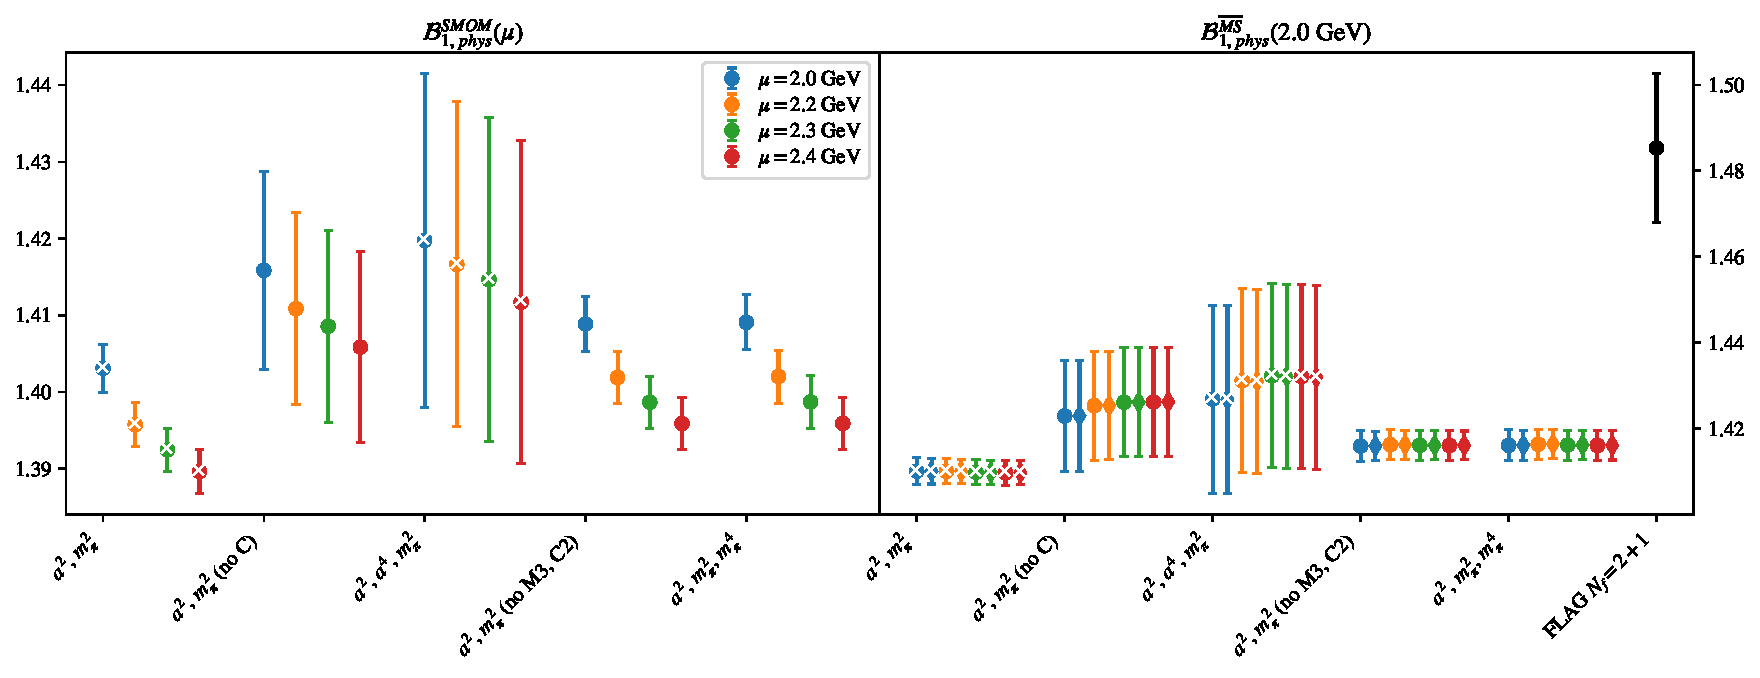
\includegraphics[page=1, width=1.1\textwidth]{VVpAA/SUSY/fit_summary_bag.pdf}
\caption{$\mathcal{B}_{1}$\\(left) $\mathcal{B}_{phys}$ in RI/SMOM scheme from fit variations (fits with $p$-value $<0.05$ marked with ``$\times$"). \\(right) $\mathcal{B}_{phys}$ in $\overline{MS}$ computed using $\mathcal{B}^{\overline{MS}} = R^{\overline{MS}\leftarrow SMOM}(2.0)\sigma_{npt}(2.0,\mu) \mathcal{B}^{SMOM}(\mu)$.}
\end{figure}
\clearpage
\begin{figure}
\centering
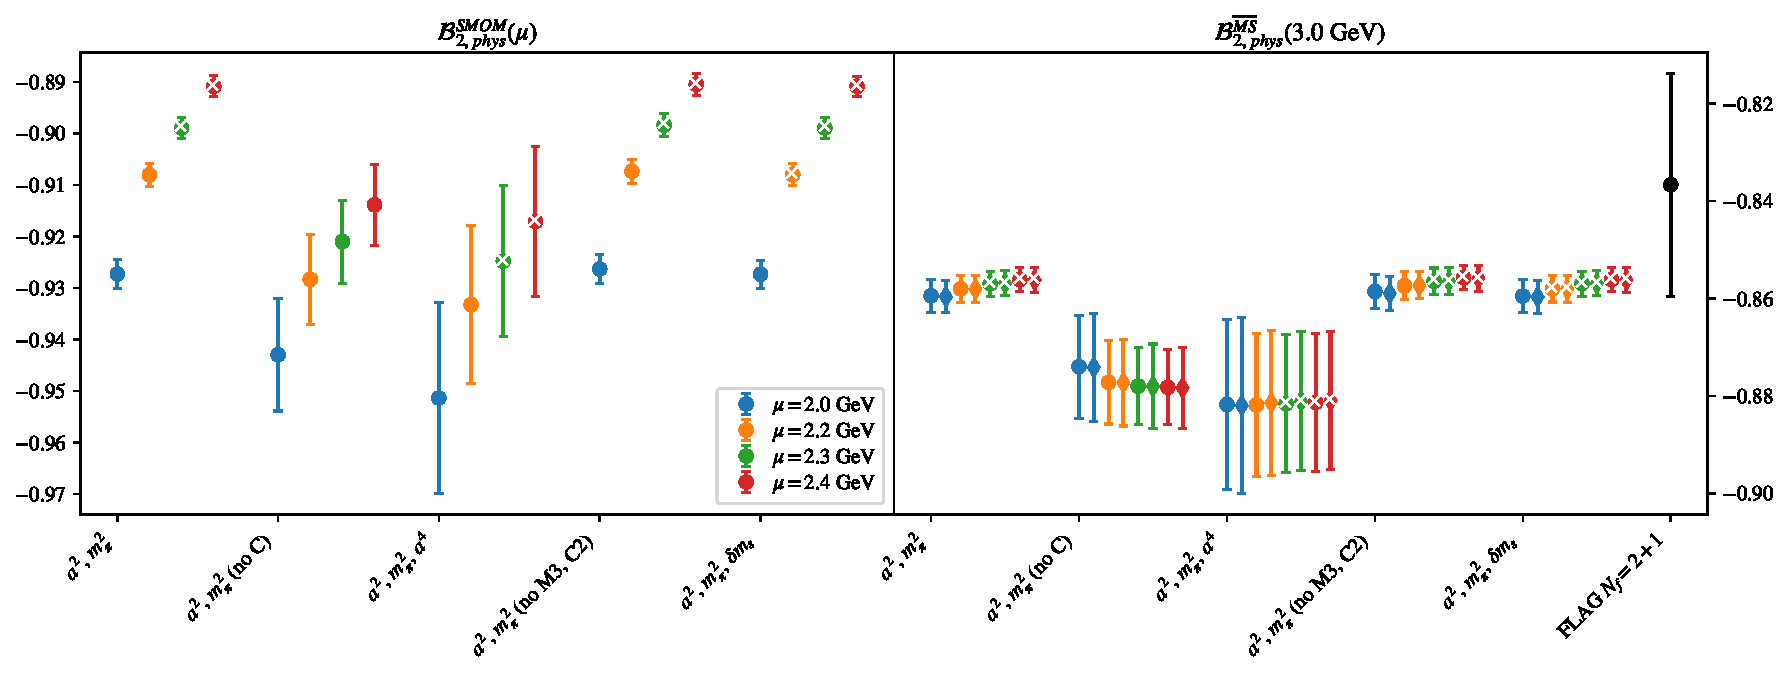
\includegraphics[page=1, width=1.1\textwidth]{VVmAA/SUSY/fit_summary_bag.pdf}
\caption{$\mathcal{B}_{2}$\\(left) $\mathcal{B}_{phys}$ in RI/SMOM scheme from fit variations (fits with $p$-value $<0.05$ marked with ``$\times$"). \\(right) $\mathcal{B}_{phys}$ in $\overline{MS}$ computed using $\mathcal{B}^{\overline{MS}} = R^{\overline{MS}\leftarrow SMOM}(3.0)\sigma_{npt}(3.0,\mu) \mathcal{B}^{SMOM}(\mu)$.}
\end{figure}
\clearpage
\begin{figure}
\centering
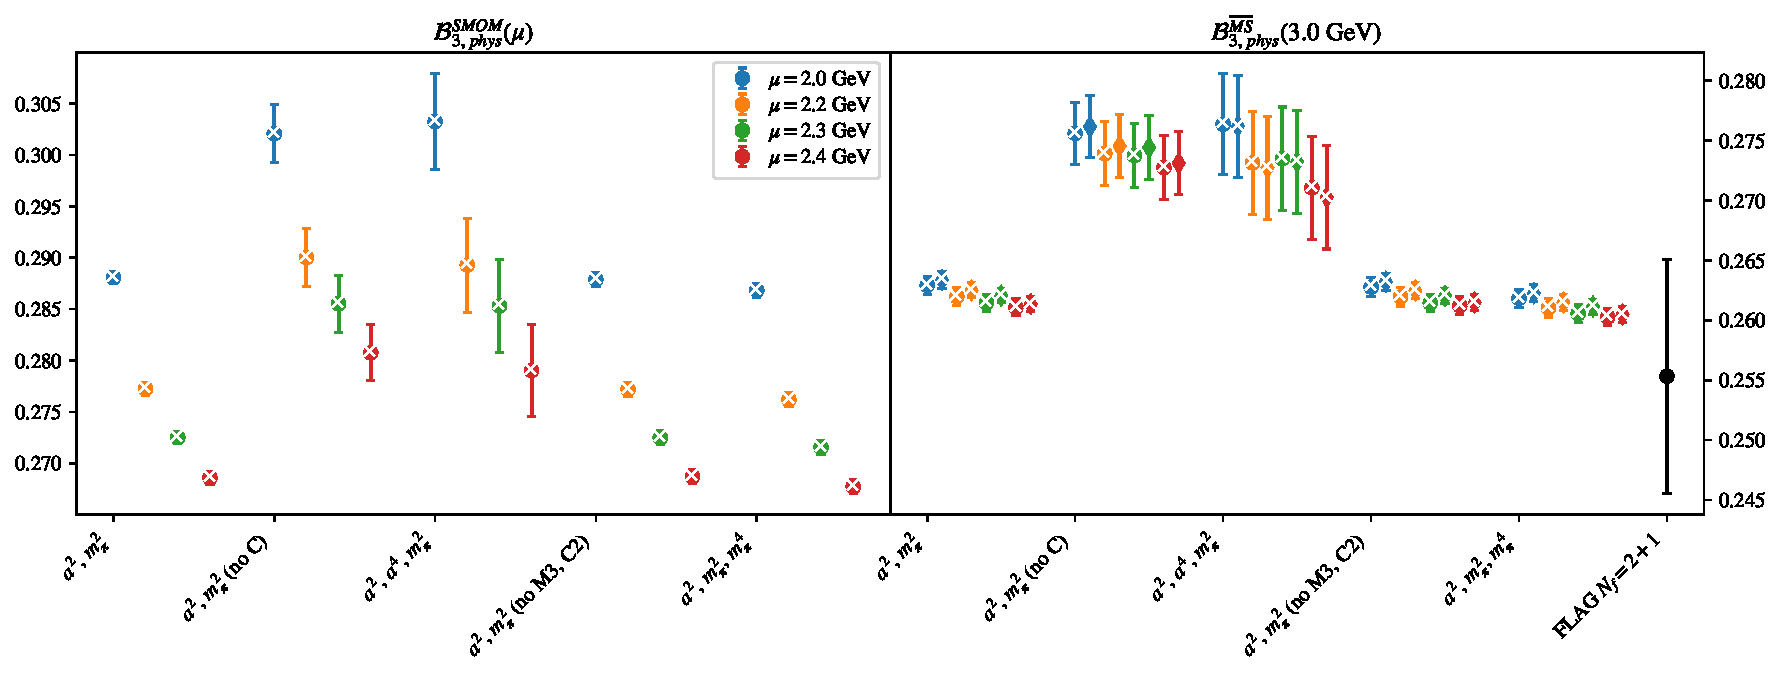
\includegraphics[page=1, width=1.1\textwidth]{SSmPP/SUSY/fit_summary_bag.pdf}
\caption{$\mathcal{B}_{3}$\\(left) $\mathcal{B}_{phys}$ in RI/SMOM scheme from fit variations (fits with $p$-value $<0.05$ marked with ``$\times$"). \\(right) $\mathcal{B}_{phys}$ in $\overline{MS}$ computed using $\mathcal{B}^{\overline{MS}} = R^{\overline{MS}\leftarrow SMOM}(3.0)\sigma_{npt}(3.0,\mu) \mathcal{B}^{SMOM}(\mu)$.}
\end{figure}
\clearpage
\begin{figure}
\centering
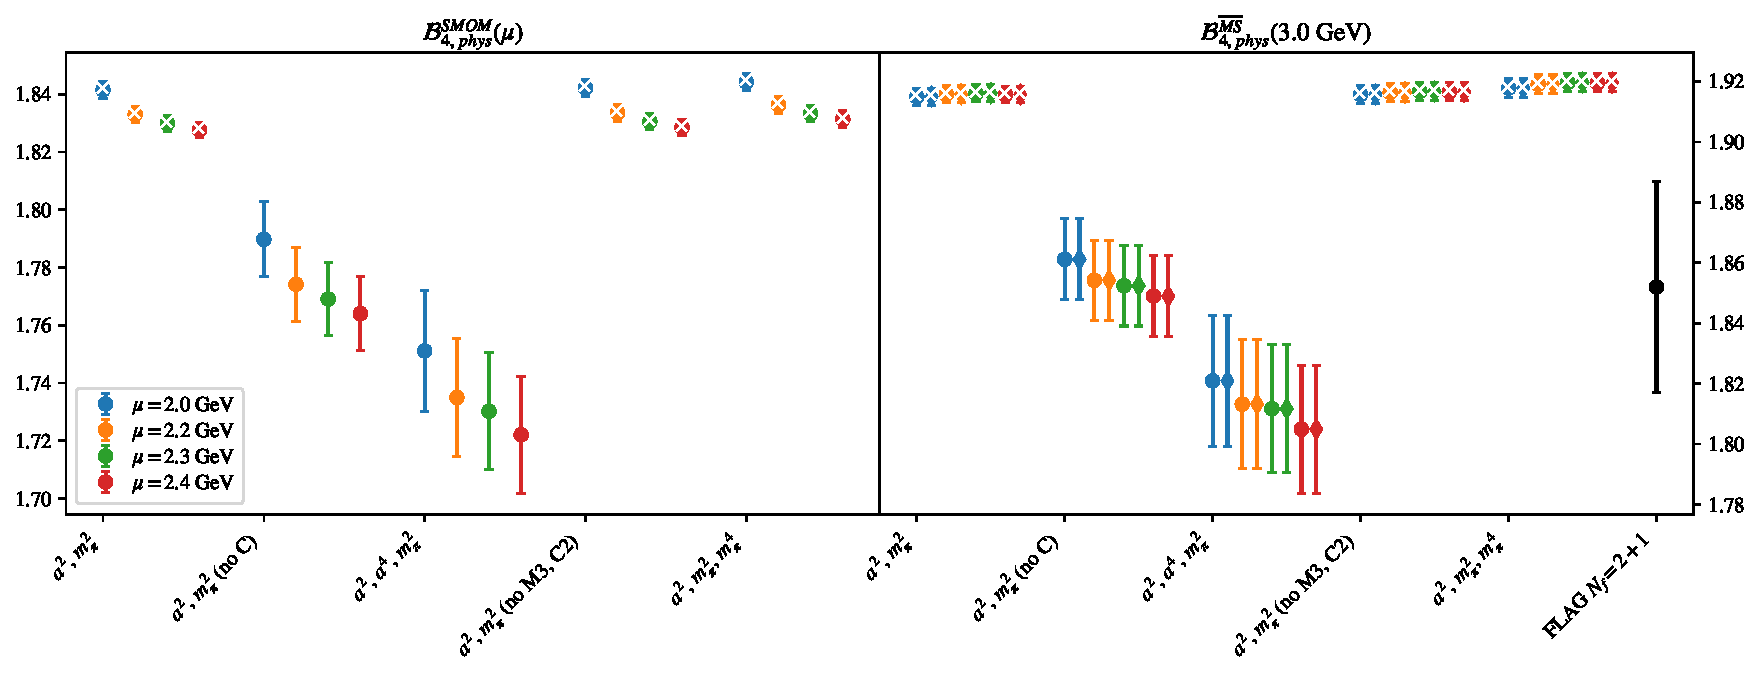
\includegraphics[page=1, width=1.1\textwidth]{SSpPP/SUSY/fit_summary_bag.pdf}
\caption{$\mathcal{B}_{4}$\\(left) $\mathcal{B}_{phys}$ in RI/SMOM scheme from fit variations (fits with $p$-value $<0.05$ marked with ``$\times$"). \\(right) $\mathcal{B}_{phys}$ in $\overline{MS}$ computed using $\mathcal{B}^{\overline{MS}} = R^{\overline{MS}\leftarrow SMOM}(3.0)\sigma_{npt}(3.0,\mu) \mathcal{B}^{SMOM}(\mu)$.}
\end{figure}
\clearpage
\begin{figure}
\centering
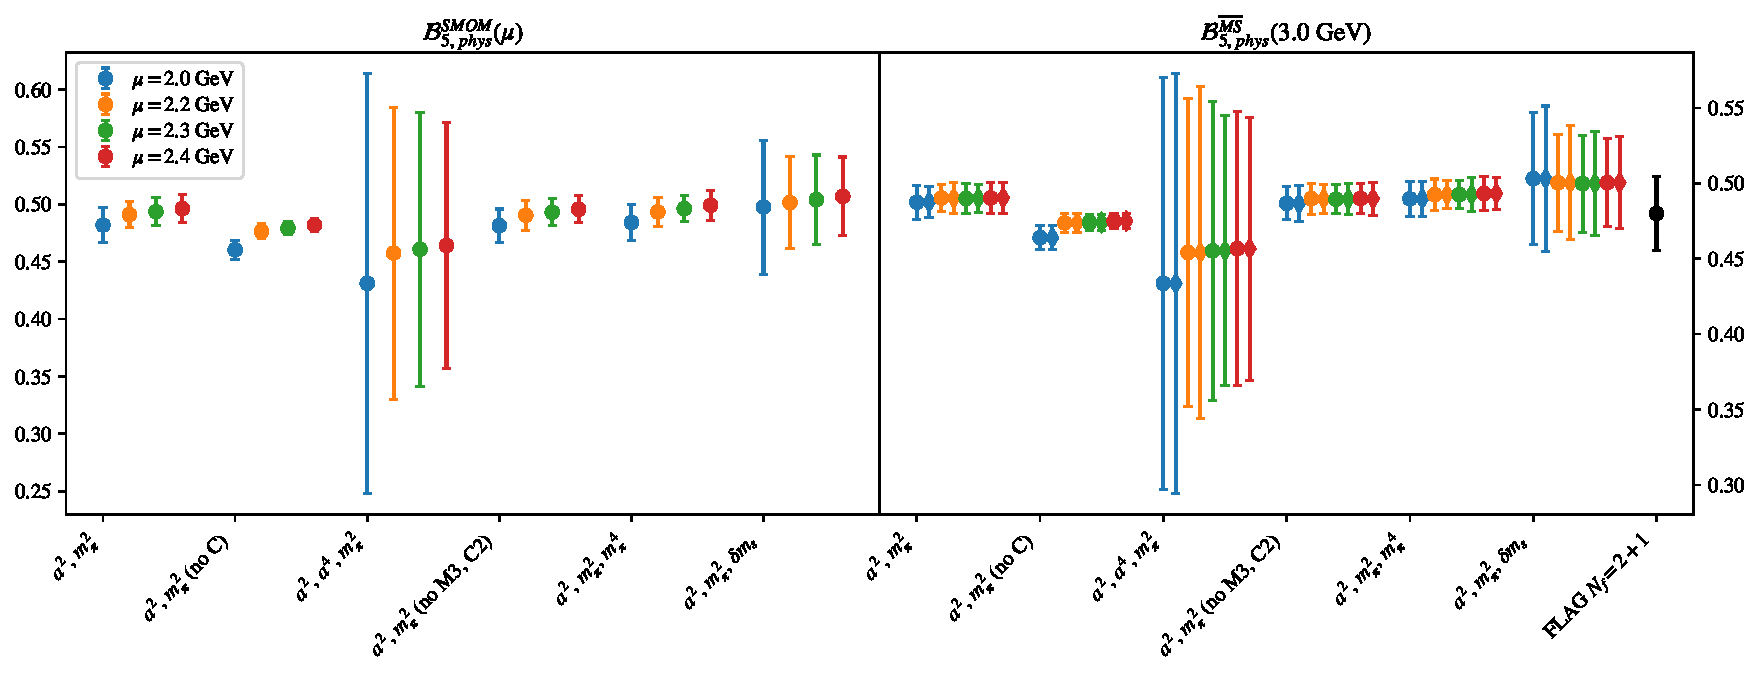
\includegraphics[page=1, width=1.1\textwidth]{TT/SUSY/fit_summary_bag.pdf}
\caption{$\mathcal{B}_{5}$\\(left) $\mathcal{B}_{phys}$ in RI/SMOM scheme from fit variations (fits with $p$-value $<0.05$ marked with ``$\times$"). \\(right) $\mathcal{B}_{phys}$ in $\overline{MS}$ computed using $\mathcal{B}^{\overline{MS}} = R^{\overline{MS}\leftarrow SMOM}(3.0)\sigma_{npt}(3.0,\mu) \mathcal{B}^{SMOM}(\mu)$.}
\end{figure}
\clearpage
\section{$\mathcal{B}_1$}
\begin{table}[h!]
\begin{center}
\begin{tabular}{|c|c|c|c|c|c|c|}
\hline
$\mu$ (GeV) & $a^2$, $m_\pi^2$& $a^2$, $m_\pi^2$ (no C)& $a^2$, $m_\pi^2$, $a^4$& $a^2$, $m_\pi^2$ (no M3, C2)& $a^2$, $m_\pi^2$, $m_\pi^4$& $a^2$, $m_\pi^2$, $\delta m_s$\\
\hline
2.0& \hyperlink{VVpAA/SUSY/bag_a2m2_20.pdf.1}{\textbf{1.4002(32)}: 2.608 (0.023)} & \hyperlink{VVpAA/SUSY/bag_a2m2noC_20.pdf.1}{\textbf{1.436(13)}: 0.273 (0.761)} & \hyperlink{VVpAA/SUSY/bag_a2a4m2_20.pdf.1}{\textbf{1.453(22)}: 2.097 (0.078)} & \hyperlink{VVpAA/SUSY/bag_a2m2mcut_20.pdf.1}{\textbf{1.4046(33)}: 2.257 (0.08)} & \hyperlink{VVpAA/SUSY/bag_a2m2m4_20.pdf.1}{\textbf{1.4031(35)}: 2.755 (0.026)} & \hyperlink{VVpAA/SUSY/bag_a2m2delm_20.pdf.1}{\textbf{1.4008(32)}: 1.363 (0.244)}\\
2.2& \hyperlink{VVpAA/SUSY/bag_a2m2_22.pdf.1}{\textbf{1.3928(31)}: 3.087 (0.009)} & \hyperlink{VVpAA/SUSY/bag_a2m2noC_22.pdf.1}{\textbf{1.431(13)}: 0.303 (0.739)} & \hyperlink{VVpAA/SUSY/bag_a2a4m2_22.pdf.1}{\textbf{1.449(23)}: 2.242 (0.062)} & \hyperlink{VVpAA/SUSY/bag_a2m2mcut_22.pdf.1}{\textbf{1.3971(32)}: 2.457 (0.061)} & \hyperlink{VVpAA/SUSY/bag_a2m2m4_22.pdf.1}{\textbf{1.3956(34)}: 3.145 (0.014)} & \hyperlink{VVpAA/SUSY/bag_a2m2delm_22.pdf.1}{\textbf{1.3936(31)}: 1.453 (0.214)}\\
2.3& \hyperlink{VVpAA/SUSY/bag_a2m2_23.pdf.1}{\textbf{1.3889(31)}: 3.371 (0.005)} & \hyperlink{VVpAA/SUSY/bag_a2m2noC_23.pdf.1}{\textbf{1.429(13)}: 0.338 (0.713)} & \hyperlink{VVpAA/SUSY/bag_a2a4m2_23.pdf.1}{\textbf{1.447(22)}: 2.555 (0.037)} & \hyperlink{VVpAA/SUSY/bag_a2m2mcut_23.pdf.1}{\textbf{1.3939(34)}: 2.644 (0.047)} & \hyperlink{VVpAA/SUSY/bag_a2m2m4_23.pdf.1}{\textbf{1.3923(35)}: 3.247 (0.011)} & \hyperlink{VVpAA/SUSY/bag_a2m2delm_23.pdf.1}{\textbf{1.3901(31)}: 1.606 (0.17)}\\
2.4& \hyperlink{VVpAA/SUSY/bag_a2m2_24.pdf.1}{\textbf{1.3860(30)}: 3.577 (0.003)} & \hyperlink{VVpAA/SUSY/bag_a2m2noC_24.pdf.1}{\textbf{1.426(13)}: 0.341 (0.711)} & \hyperlink{VVpAA/SUSY/bag_a2a4m2_24.pdf.1}{\textbf{1.445(22)}: 2.727 (0.028)} & \hyperlink{VVpAA/SUSY/bag_a2m2mcut_24.pdf.1}{\textbf{1.3911(34)}: 2.749 (0.041)} & \hyperlink{VVpAA/SUSY/bag_a2m2m4_24.pdf.1}{\textbf{1.3893(35)}: 3.38 (0.009)} & \hyperlink{VVpAA/SUSY/bag_a2m2delm_24.pdf.1}{\textbf{1.3874(31)}: 1.611 (0.168)}\\
\hline
\end{tabular}
\caption{Physical point value from chiral and continuum extrapolation at renormalisation scale $\mu$. Entries are \textbf{value(error)}: $\chi^2/\text{DOF}$ ($p$-value).}
\end{center}
\end{table}
\begin{table}[h!]
\begin{center}
\begin{tabular}{|c c|c|c|c|c|c|c|}
\hline
$\mu$ (GeV) &  & $a^2$, $m_\pi^2$& $a^2$, $m_\pi^2$ (no C)& $a^2$, $m_\pi^2$, $a^4$& $a^2$, $m_\pi^2$ (no M3, C2)& $a^2$, $m_\pi^2$, $m_\pi^4$& $a^2$, $m_\pi^2$, $\delta m_s$\\
\hline
\multirow{3}{0.5in}{2.0} & $\alpha$ & 0.147(11)& -0.055(78)& -0.34(20)& 0.133(12)& 0.139(12)& 0.150(11)\\
 & $\beta$ & 0.00409(21)& 0.00347(43)& 0.00435(23)& 0.00338(34)& 0.0023(10)& 0.00540(52)\\
 & $\gamma$ &  &  & 0.99(42)&  & 0.000157(95)& -0.052(19)\\
\hline
\multirow{3}{0.5in}{2.2} & $\alpha$ & 0.152(11)& -0.065(77)& -0.36(21)& 0.138(11)& 0.144(12)& 0.154(11)\\
 & $\beta$ & 0.00397(21)& 0.00331(41)& 0.00427(24)& 0.00327(34)& 0.0020(10)& 0.00539(52)\\
 & $\gamma$ &  &  & 1.04(43)&  & 0.000179(92)& -0.055(18)\\
\hline
\multirow{3}{0.5in}{2.3} & $\alpha$ & 0.155(10)& -0.068(77)& -0.38(20)& 0.140(12)& 0.145(12)& 0.157(11)\\
 & $\beta$ & 0.00394(21)& 0.00327(40)& 0.00422(24)& 0.00322(35)& 0.0020(10)& 0.00542(51)\\
 & $\gamma$ &  &  & 1.08(42)&  & 0.000176(91)& -0.057(18)\\
\hline
\multirow{3}{0.5in}{2.4} & $\alpha$ & 0.157(10)& -0.070(77)& -0.39(20)& 0.140(12)& 0.147(12)& 0.157(11)\\
 & $\beta$ & 0.00392(20)& 0.00323(40)& 0.00423(24)& 0.00318(34)& 0.0019(10)& 0.00538(51)\\
 & $\gamma$ &  &  & 1.11(42)&  & 0.000185(92)& -0.056(18)\\
\hline
\end{tabular}
\caption{Fit values of coefficients in $Q = Q_{phys} + \mathbf{\alpha} a^2 + \mathbf{\beta}\left(\frac{m_\pi^2}{f_\pi^2}-\frac{m_{\pi,PDG}^2}{f_\pi^2}\right) + \gamma(\ldots)$}
\end{center}
\end{table}
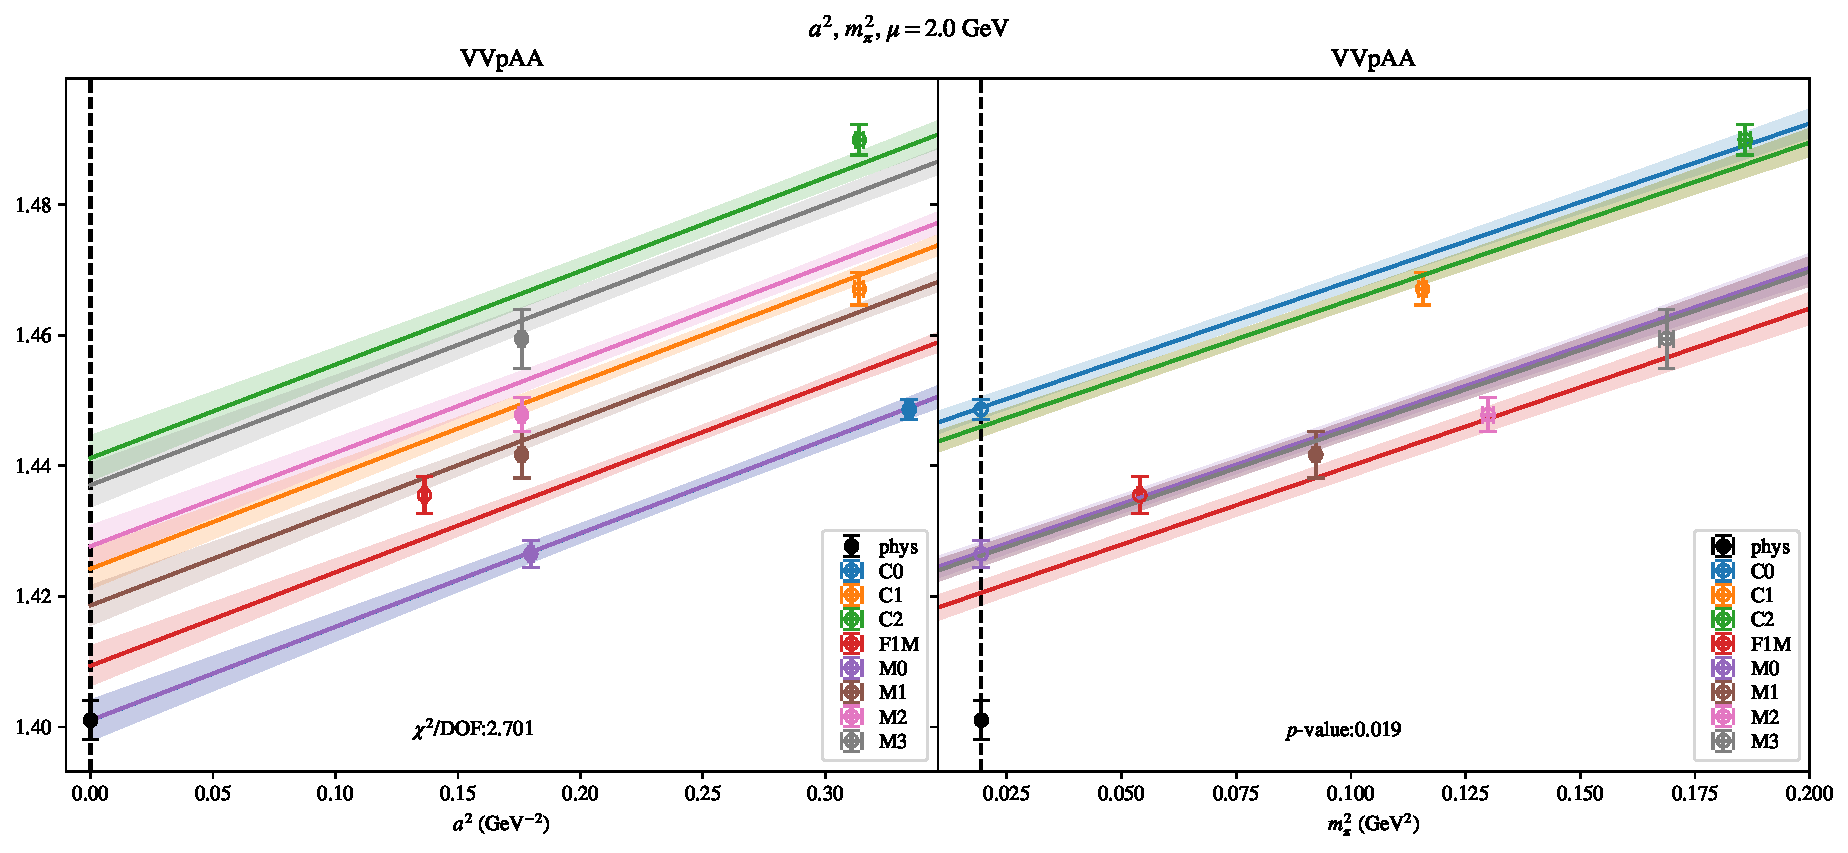
\includepdf[link, pages=-]{VVpAA/SUSY/bag_a2m2_20.pdf}
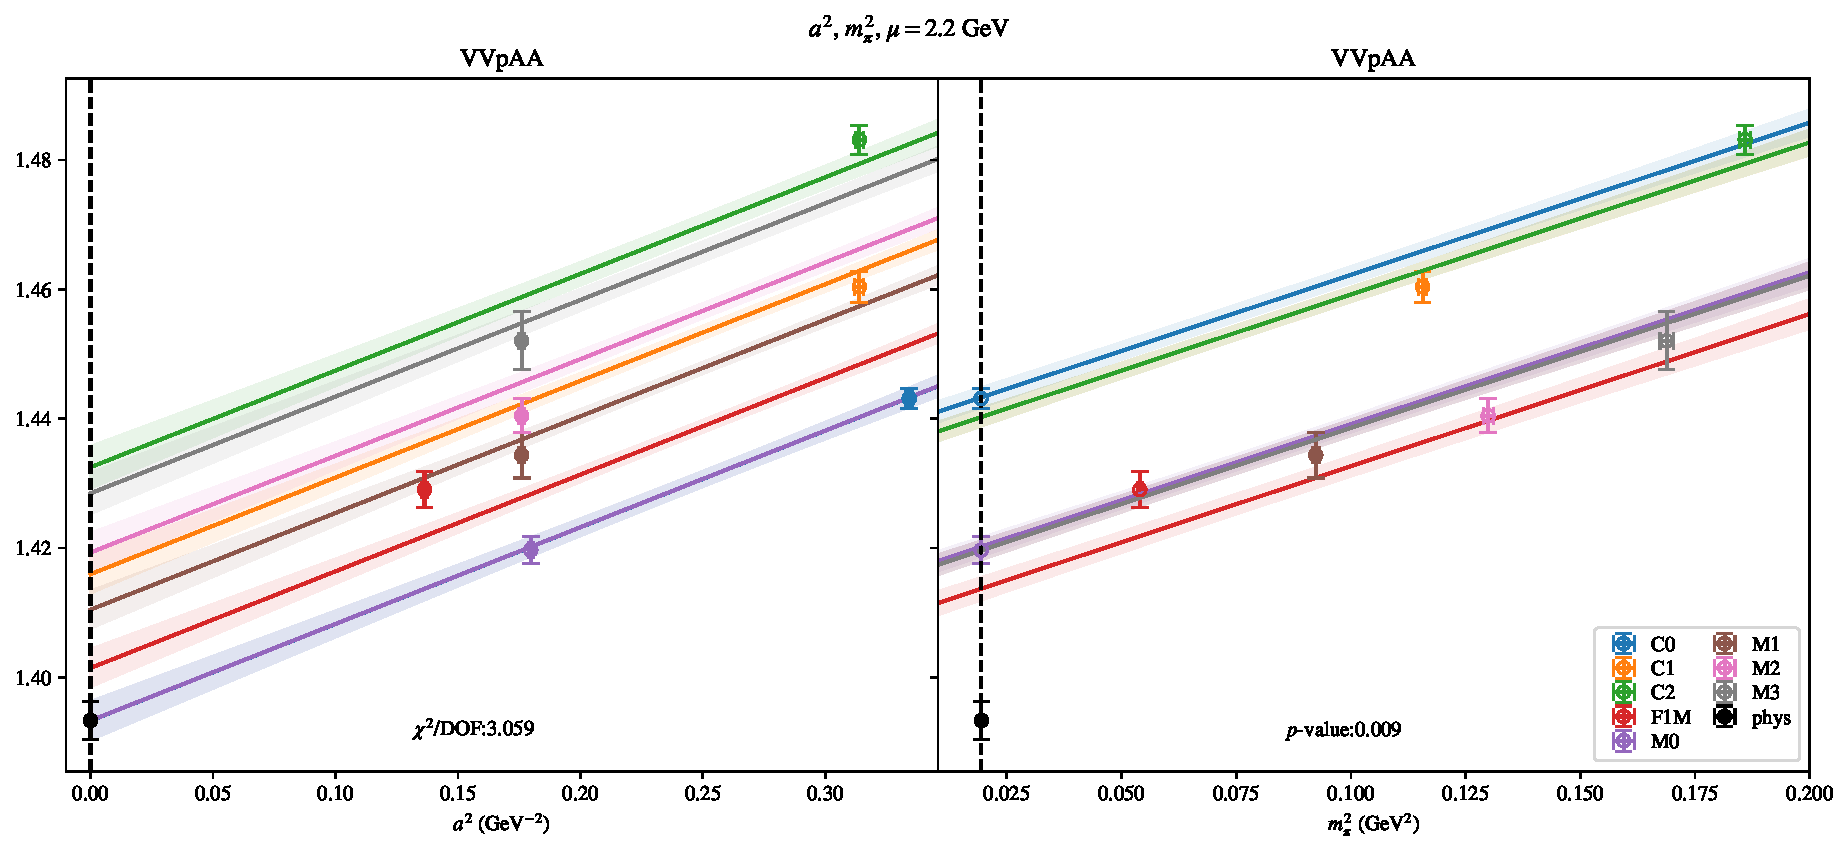
\includepdf[link, pages=-]{VVpAA/SUSY/bag_a2m2_22.pdf}
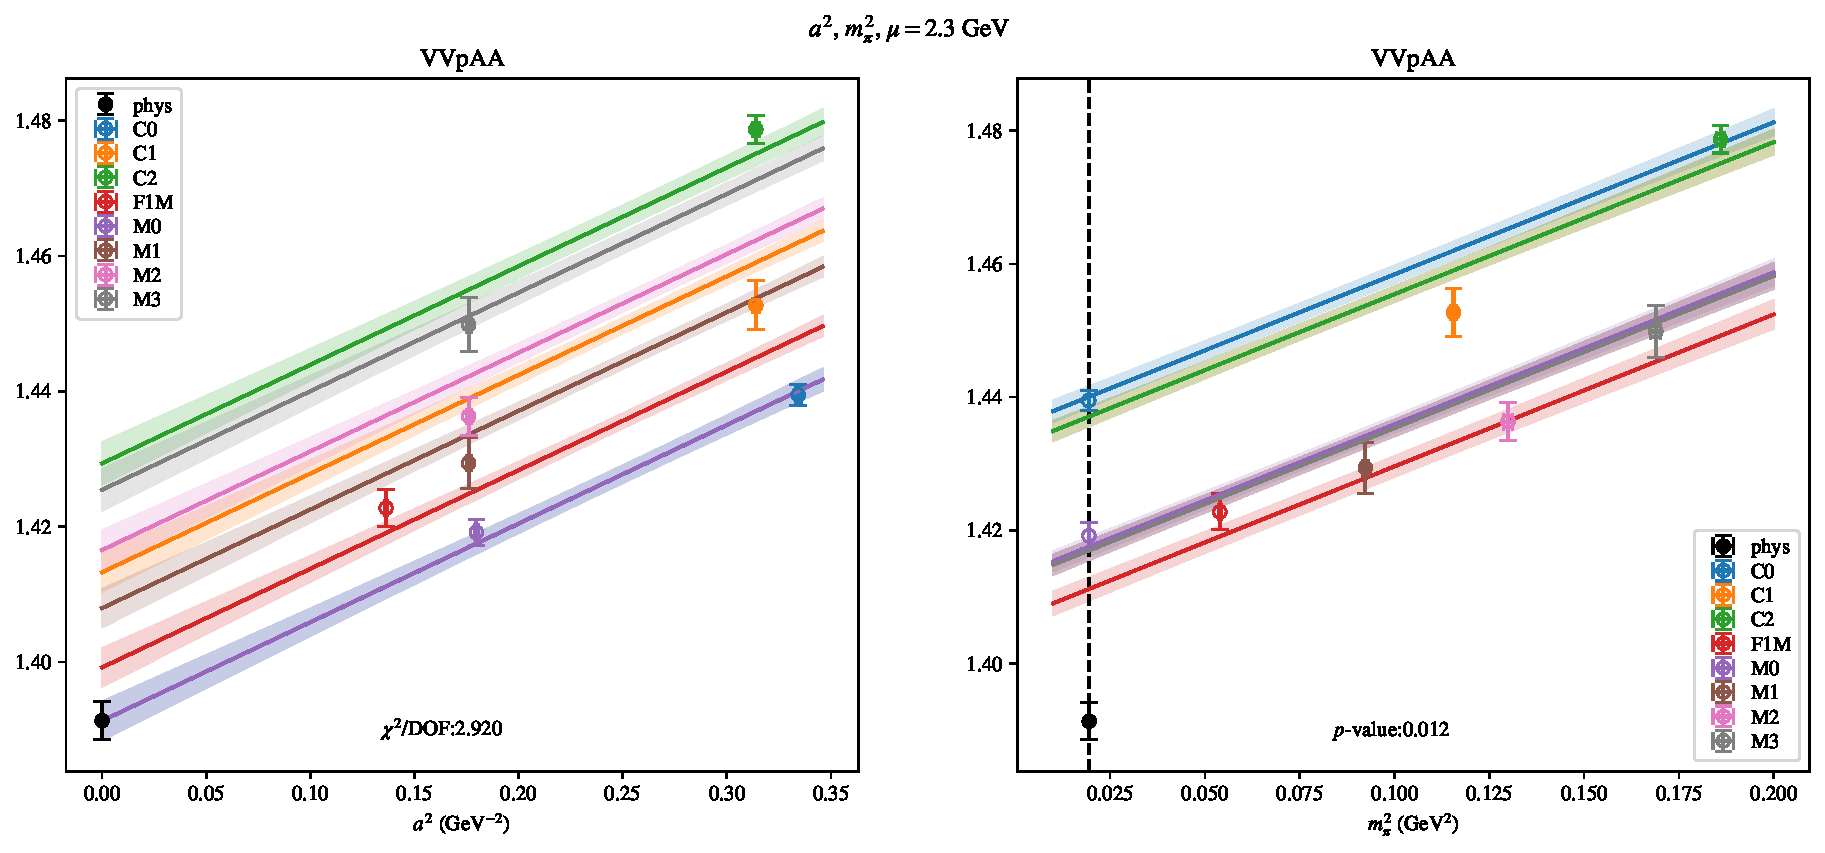
\includepdf[link, pages=-]{VVpAA/SUSY/bag_a2m2_23.pdf}
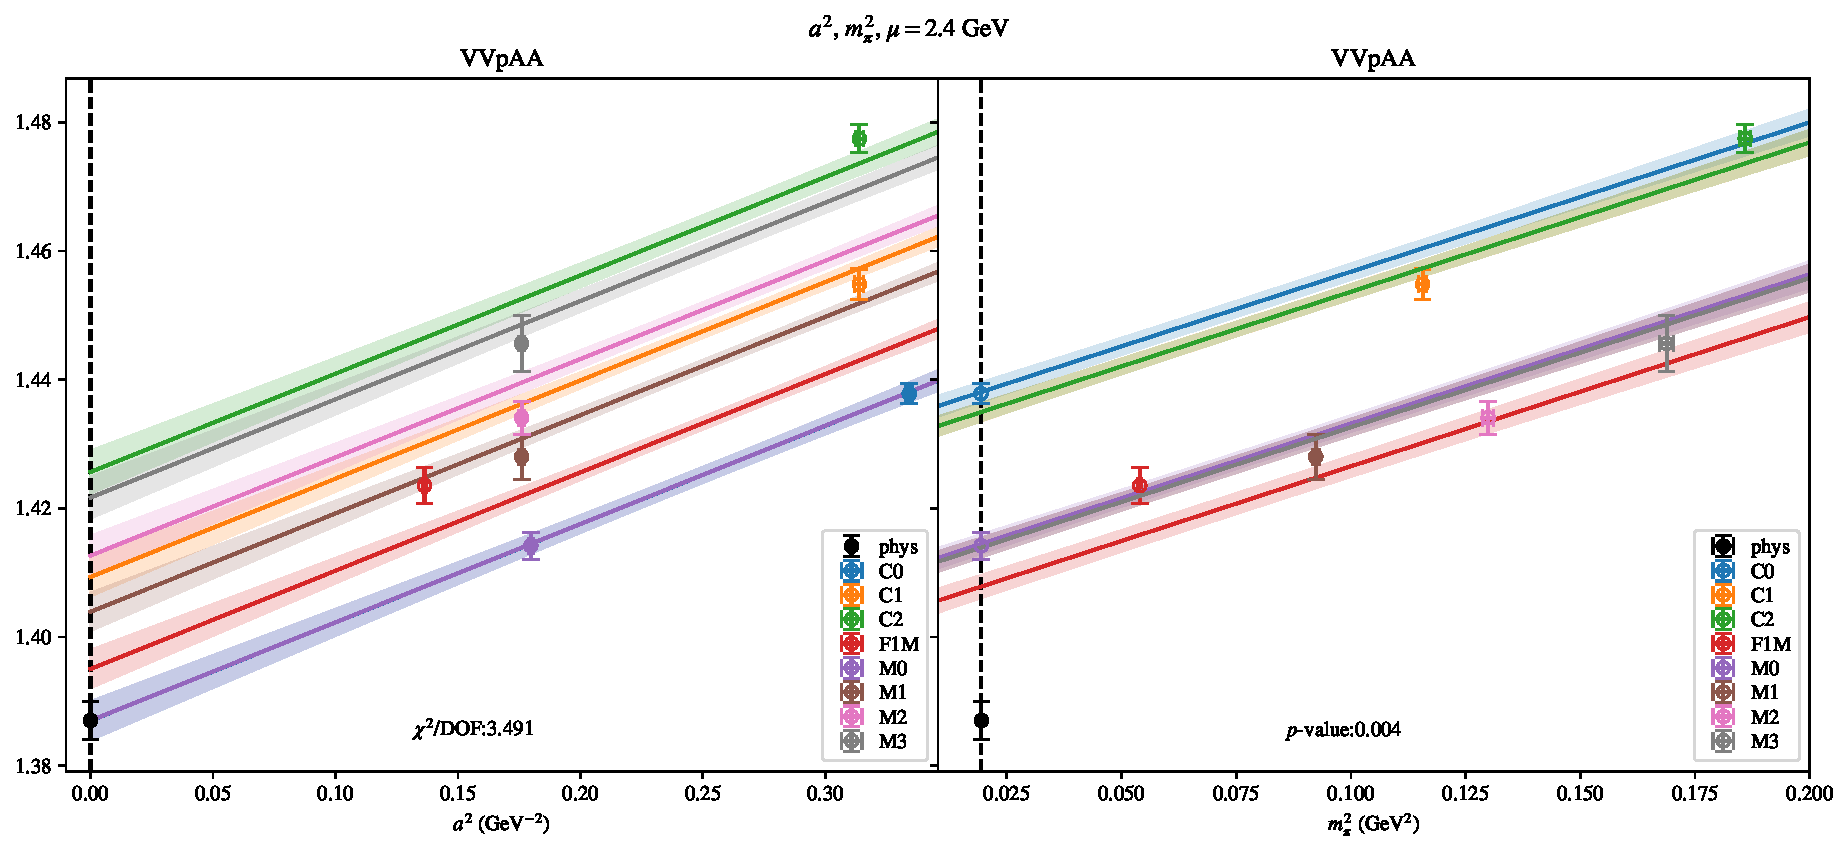
\includepdf[link, pages=-]{VVpAA/SUSY/bag_a2m2_24.pdf}
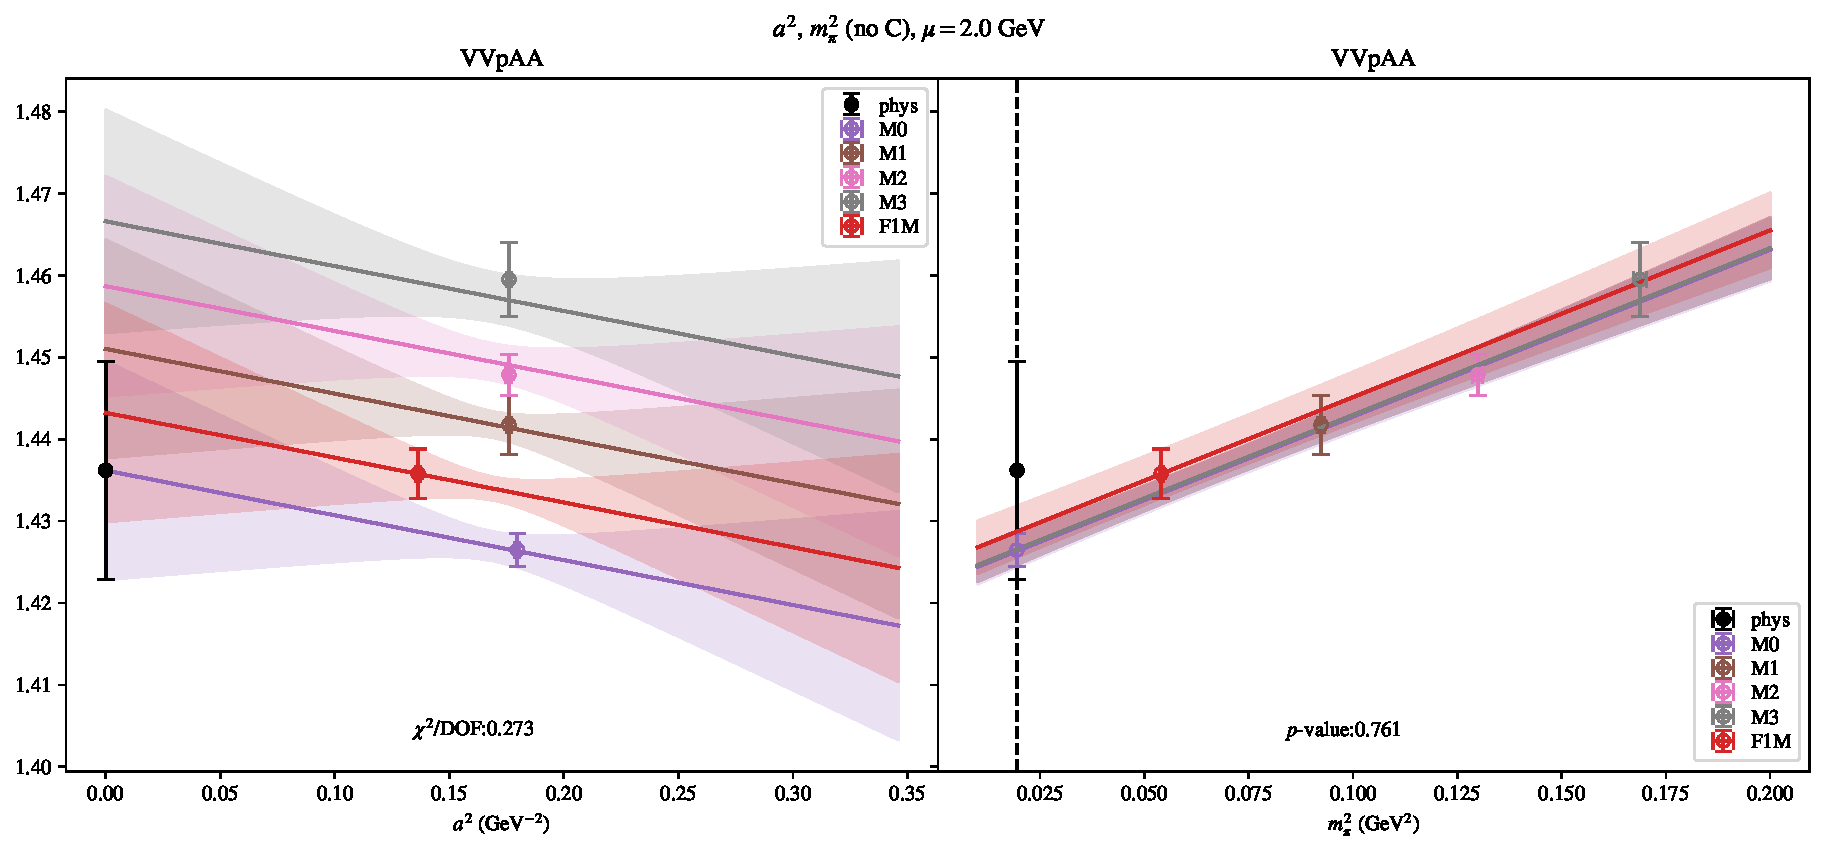
\includepdf[link, pages=-]{VVpAA/SUSY/bag_a2m2noC_20.pdf}
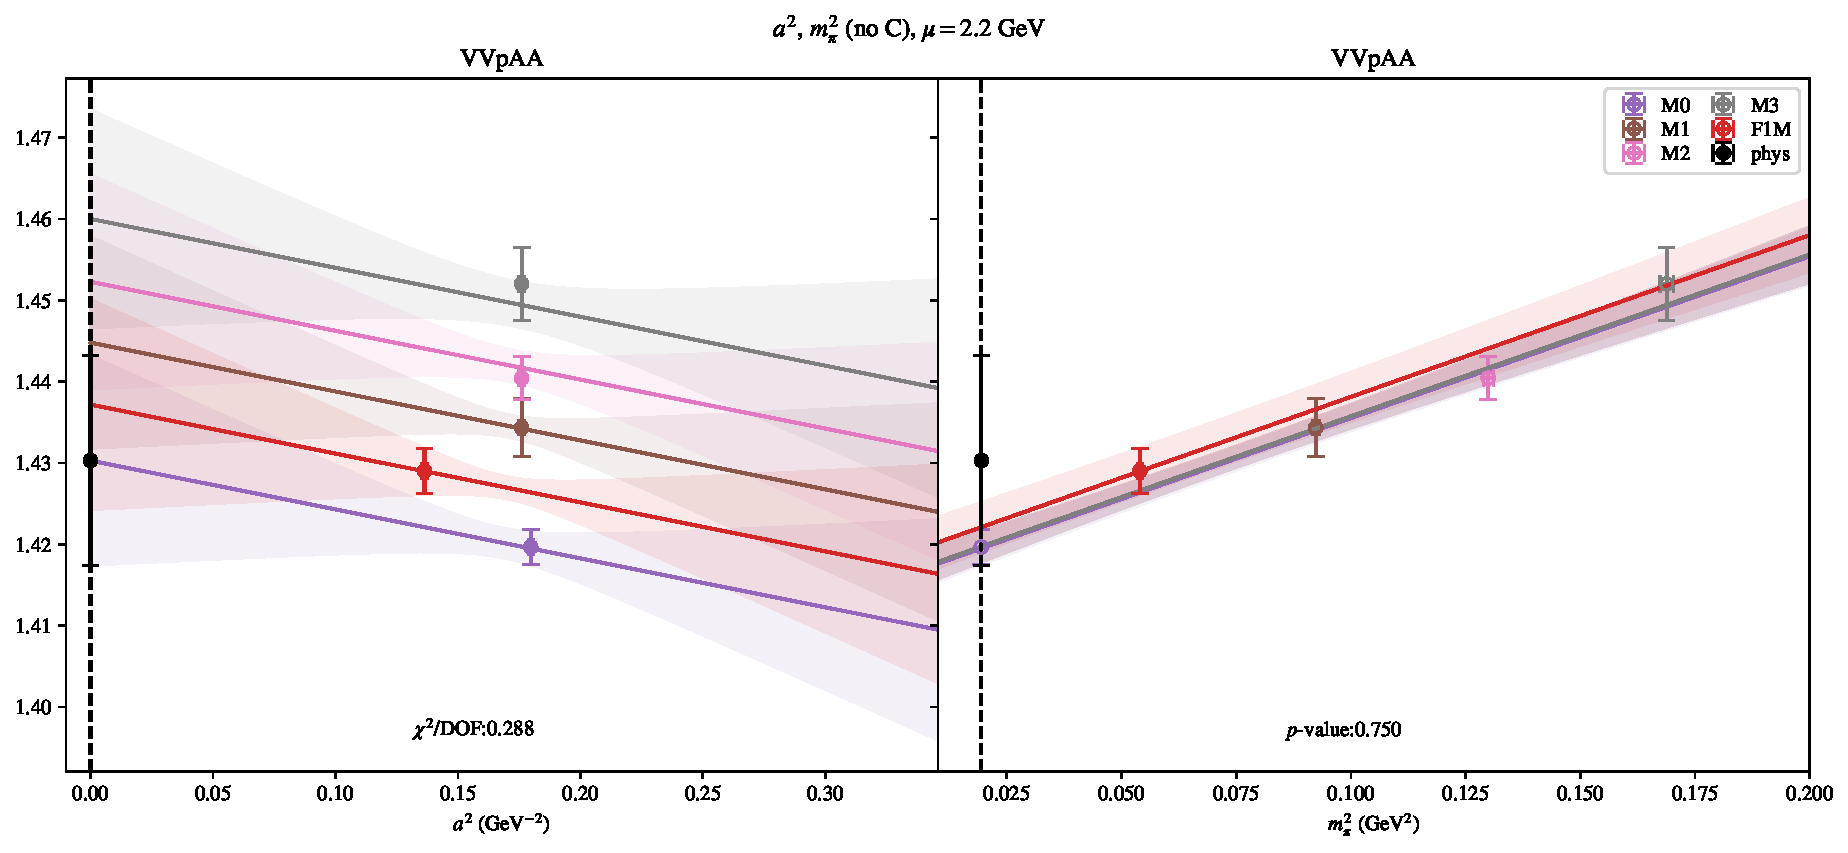
\includepdf[link, pages=-]{VVpAA/SUSY/bag_a2m2noC_22.pdf}
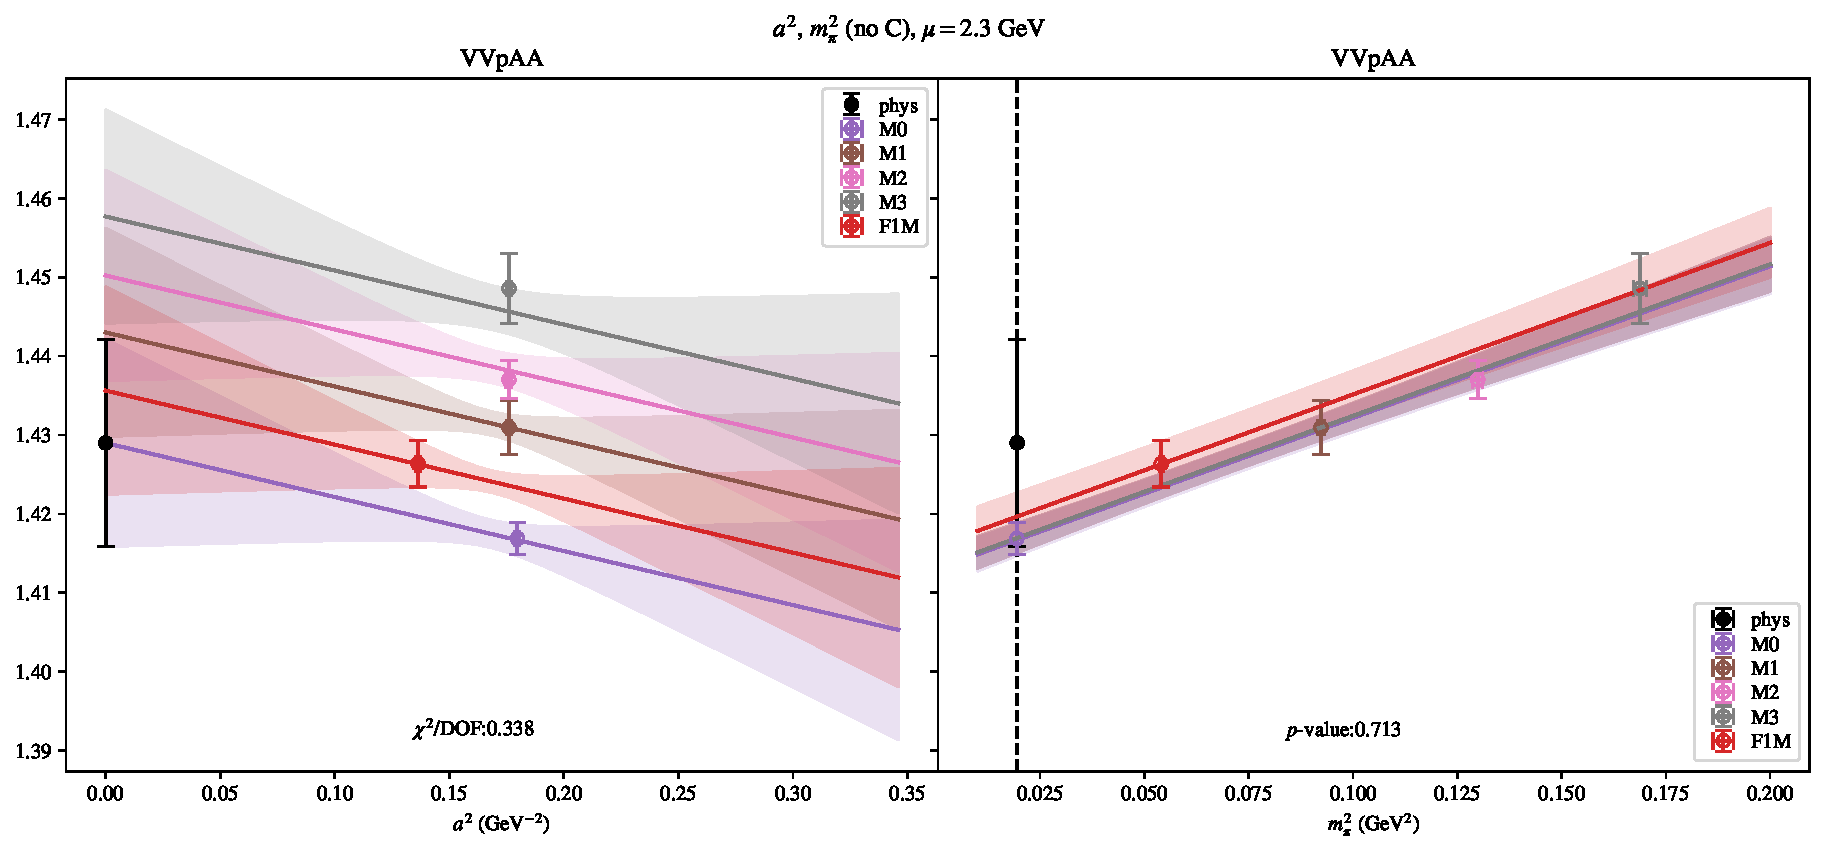
\includepdf[link, pages=-]{VVpAA/SUSY/bag_a2m2noC_23.pdf}
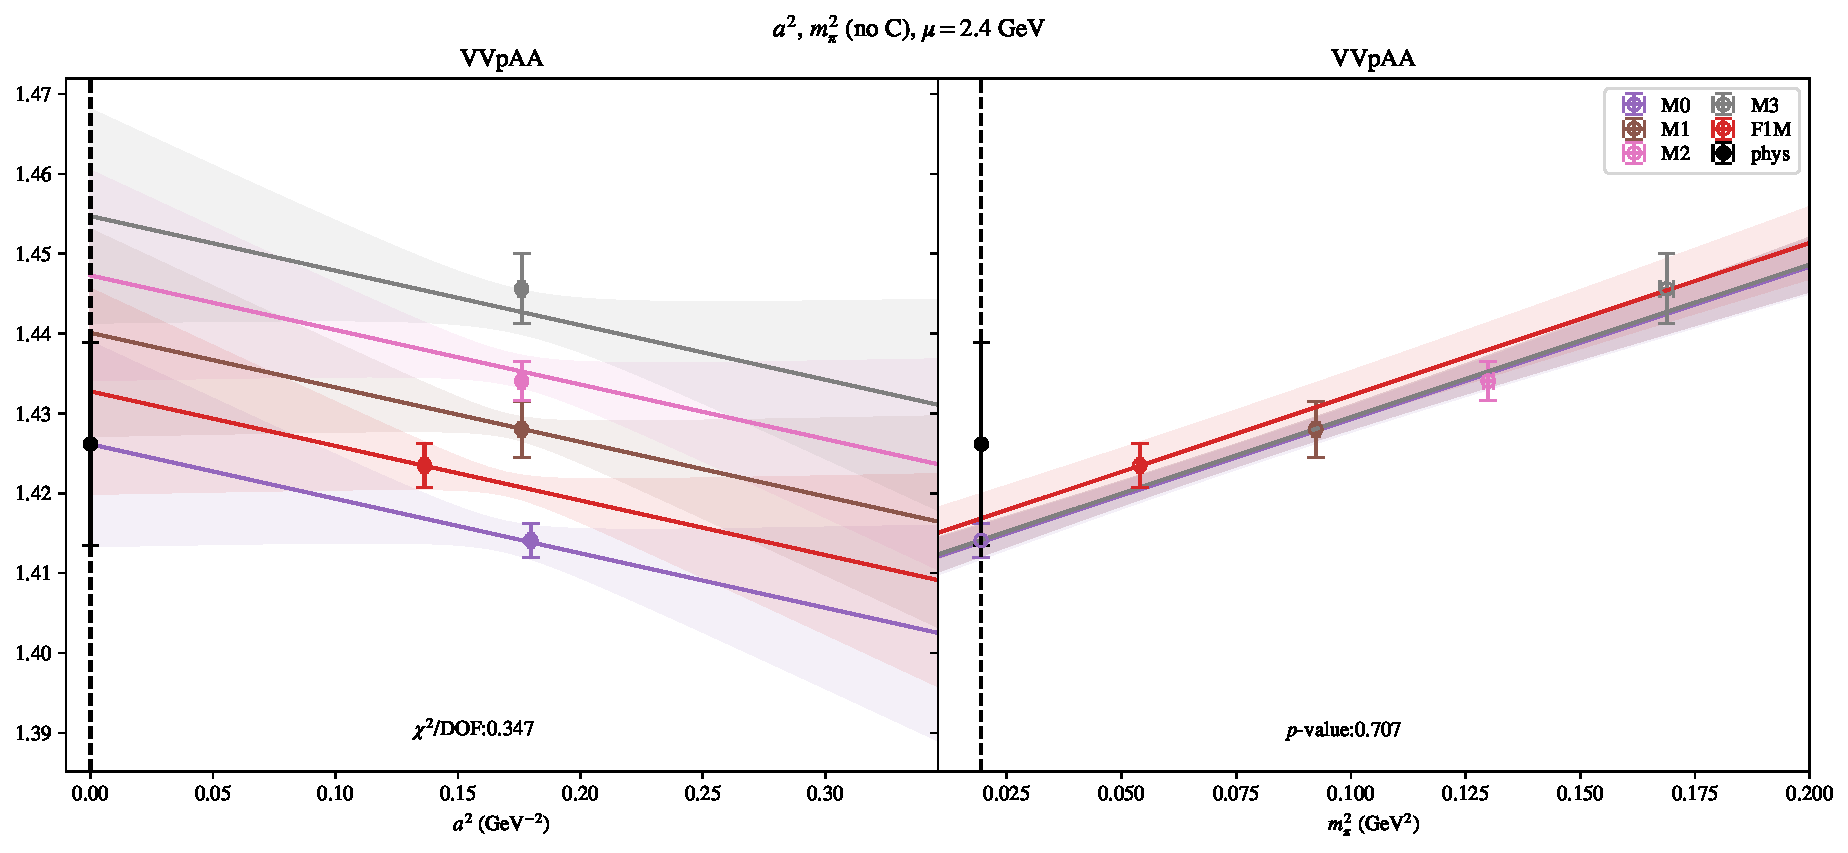
\includepdf[link, pages=-]{VVpAA/SUSY/bag_a2m2noC_24.pdf}
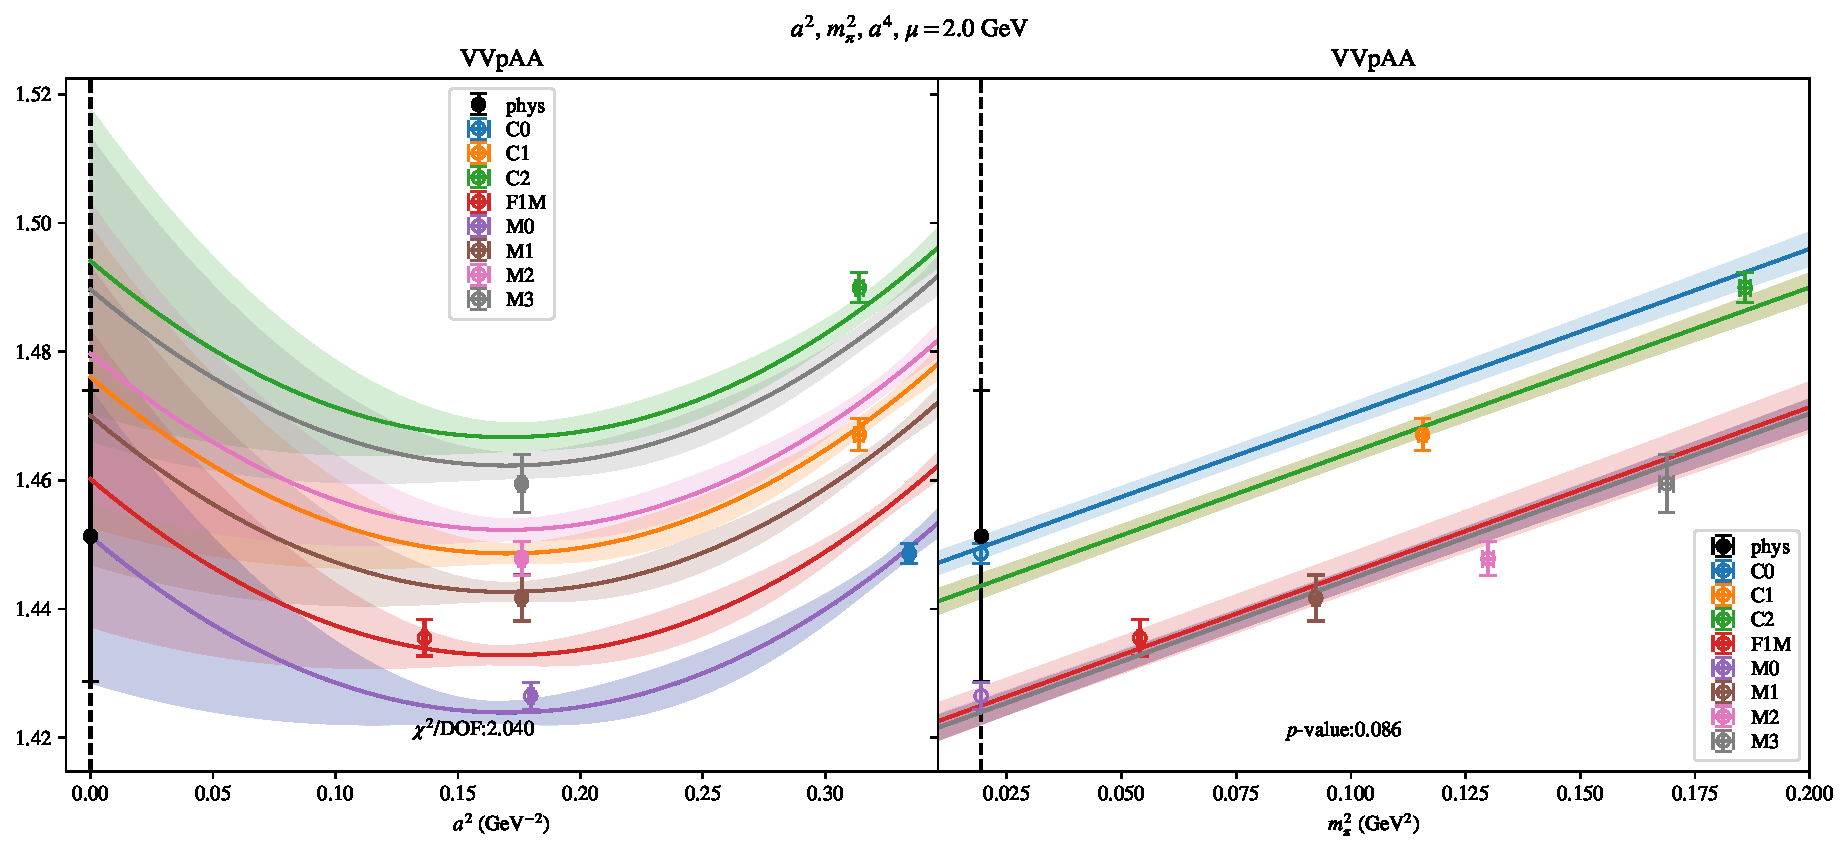
\includepdf[link, pages=-]{VVpAA/SUSY/bag_a2a4m2_20.pdf}
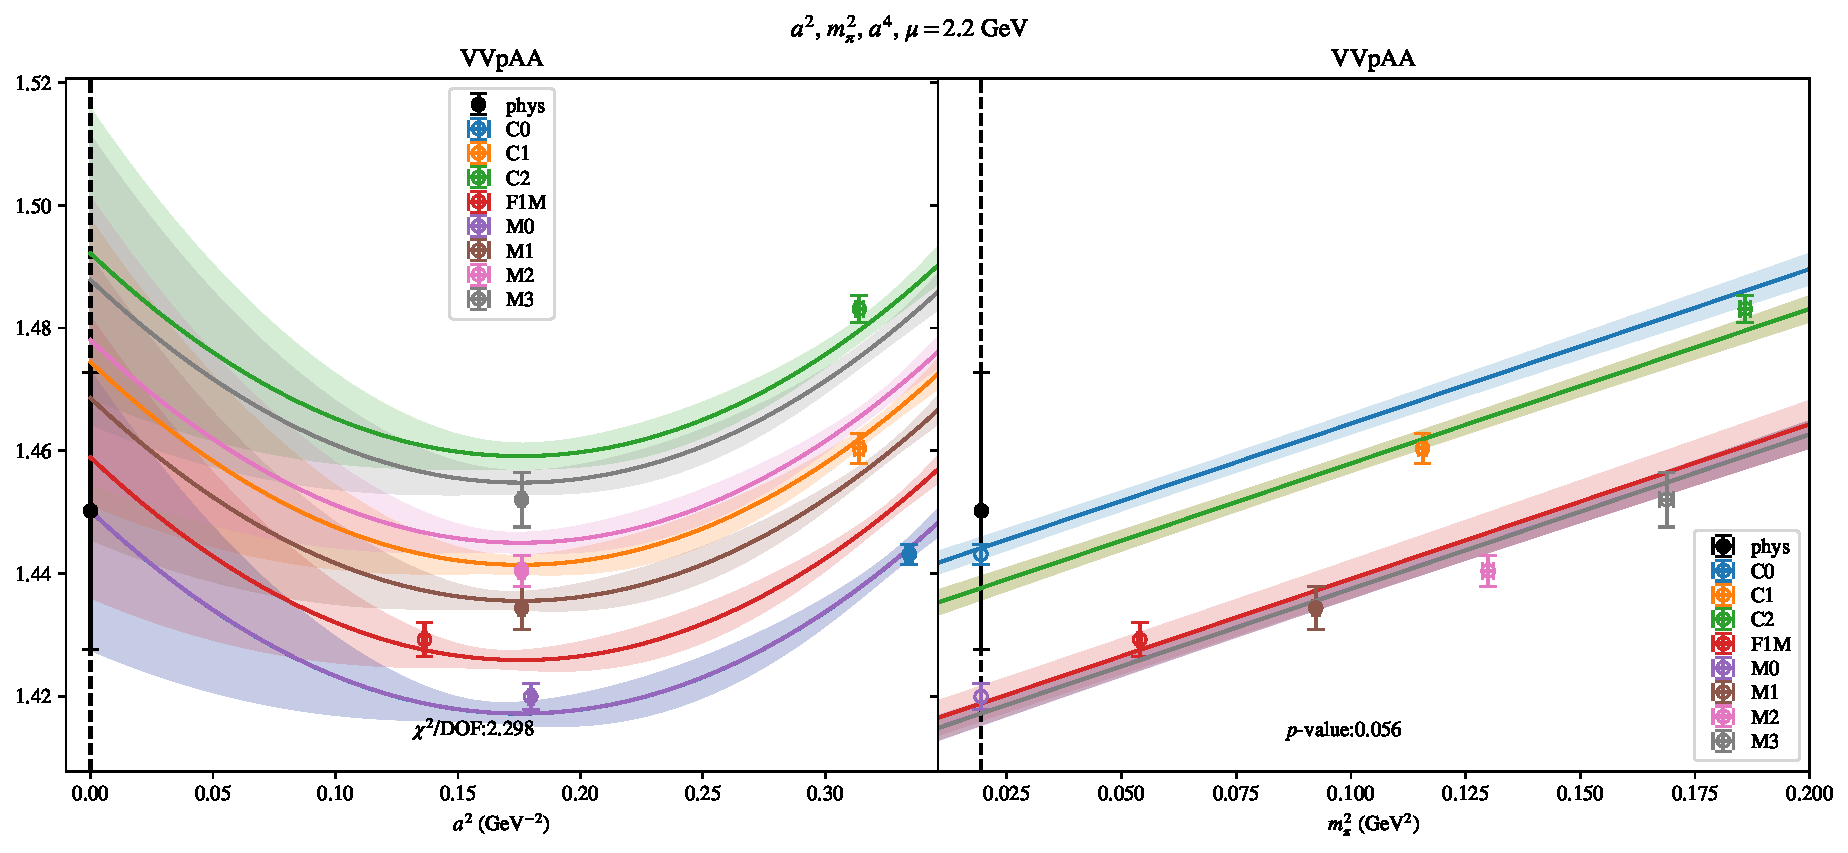
\includepdf[link, pages=-]{VVpAA/SUSY/bag_a2a4m2_22.pdf}
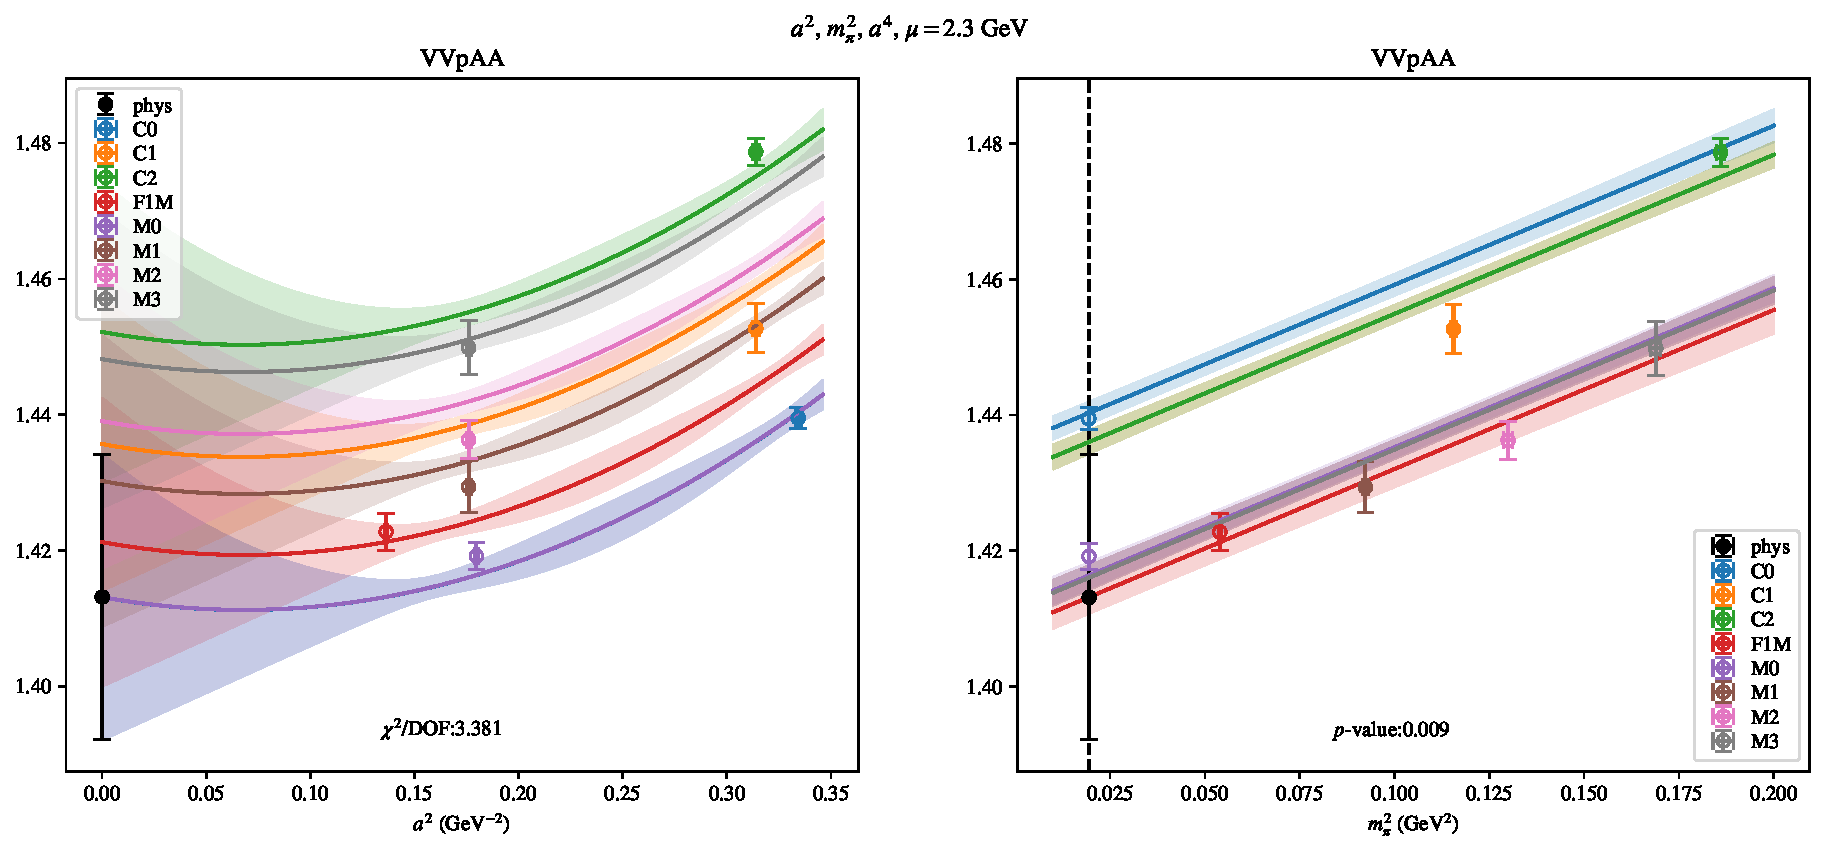
\includepdf[link, pages=-]{VVpAA/SUSY/bag_a2a4m2_23.pdf}
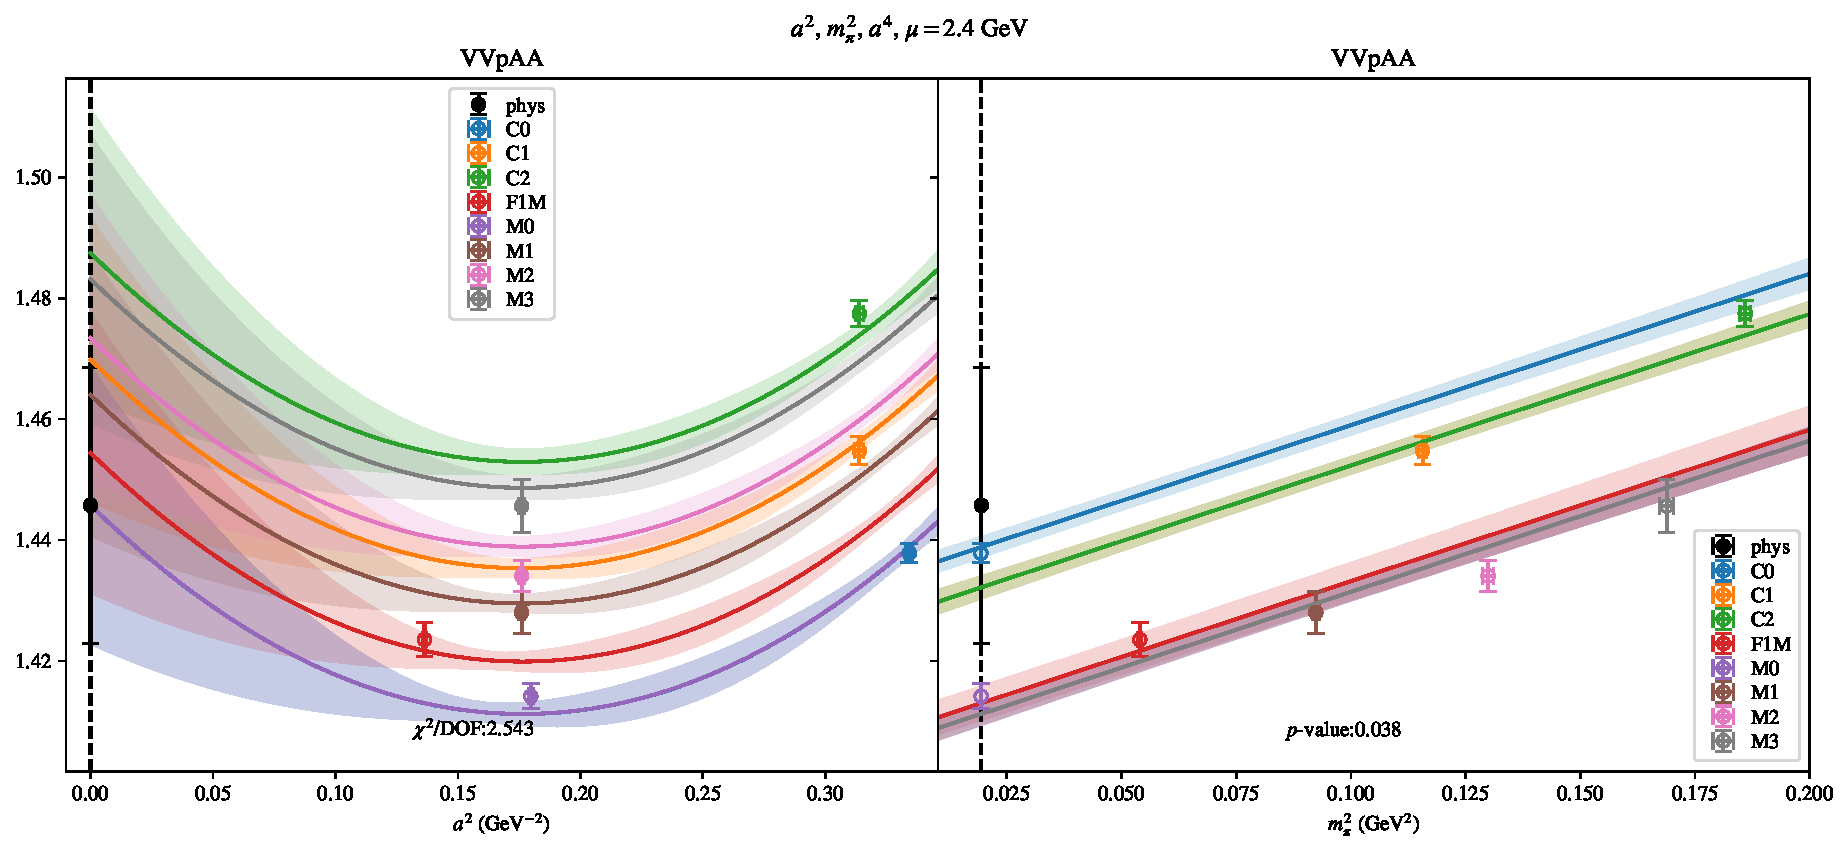
\includepdf[link, pages=-]{VVpAA/SUSY/bag_a2a4m2_24.pdf}
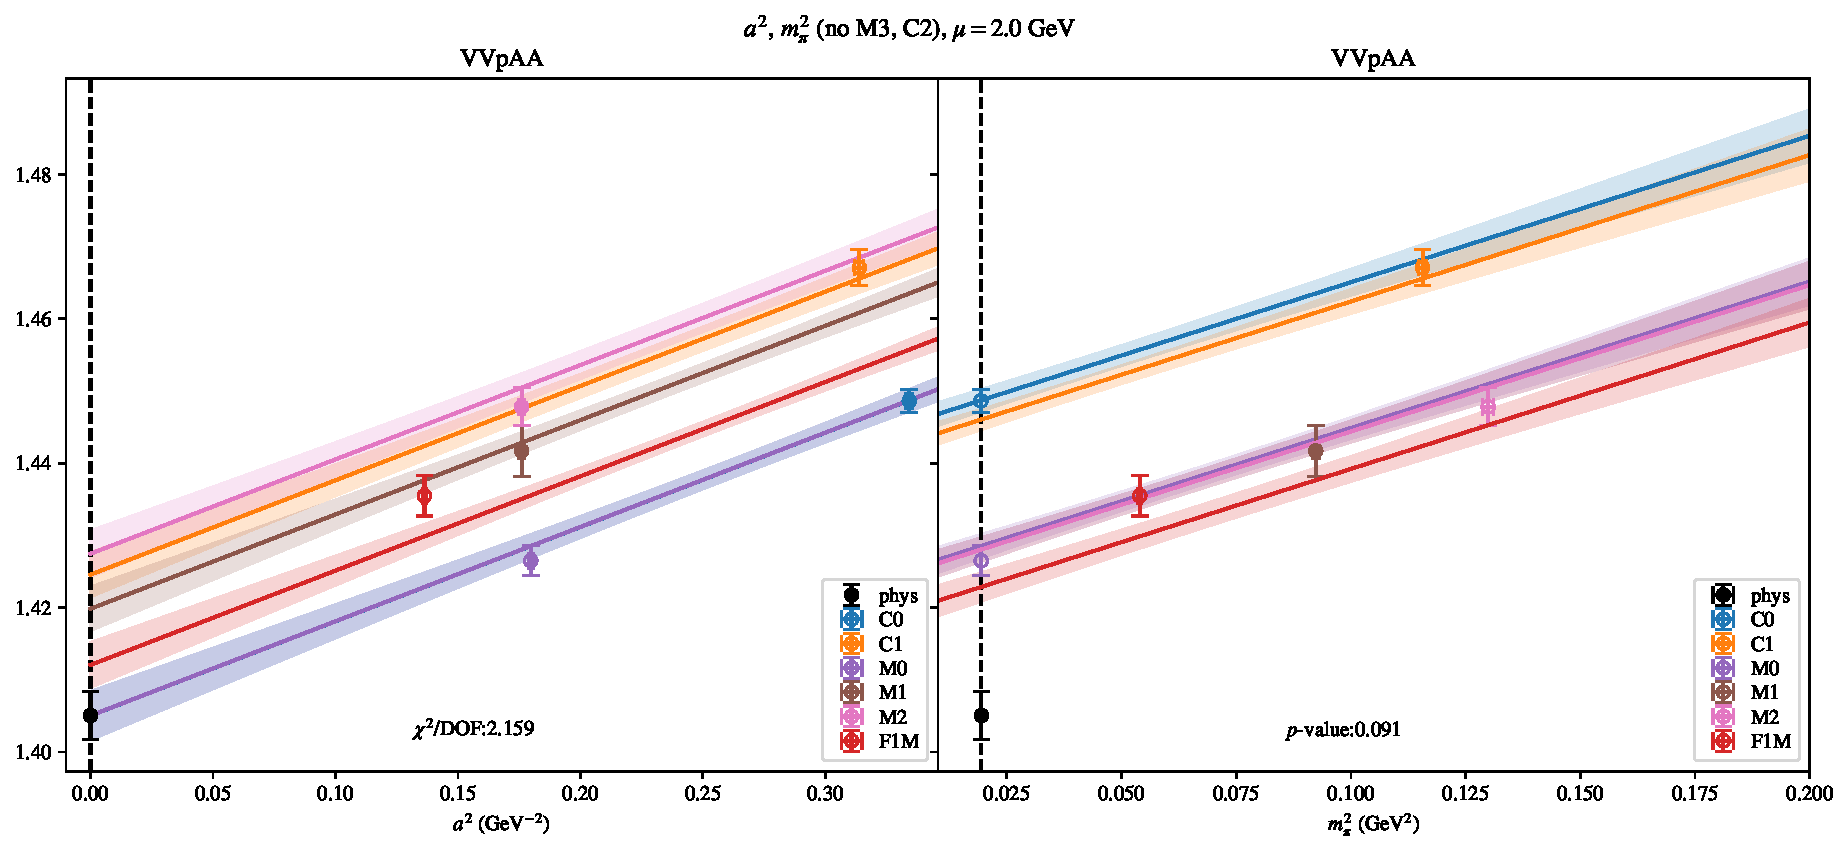
\includepdf[link, pages=-]{VVpAA/SUSY/bag_a2m2mcut_20.pdf}
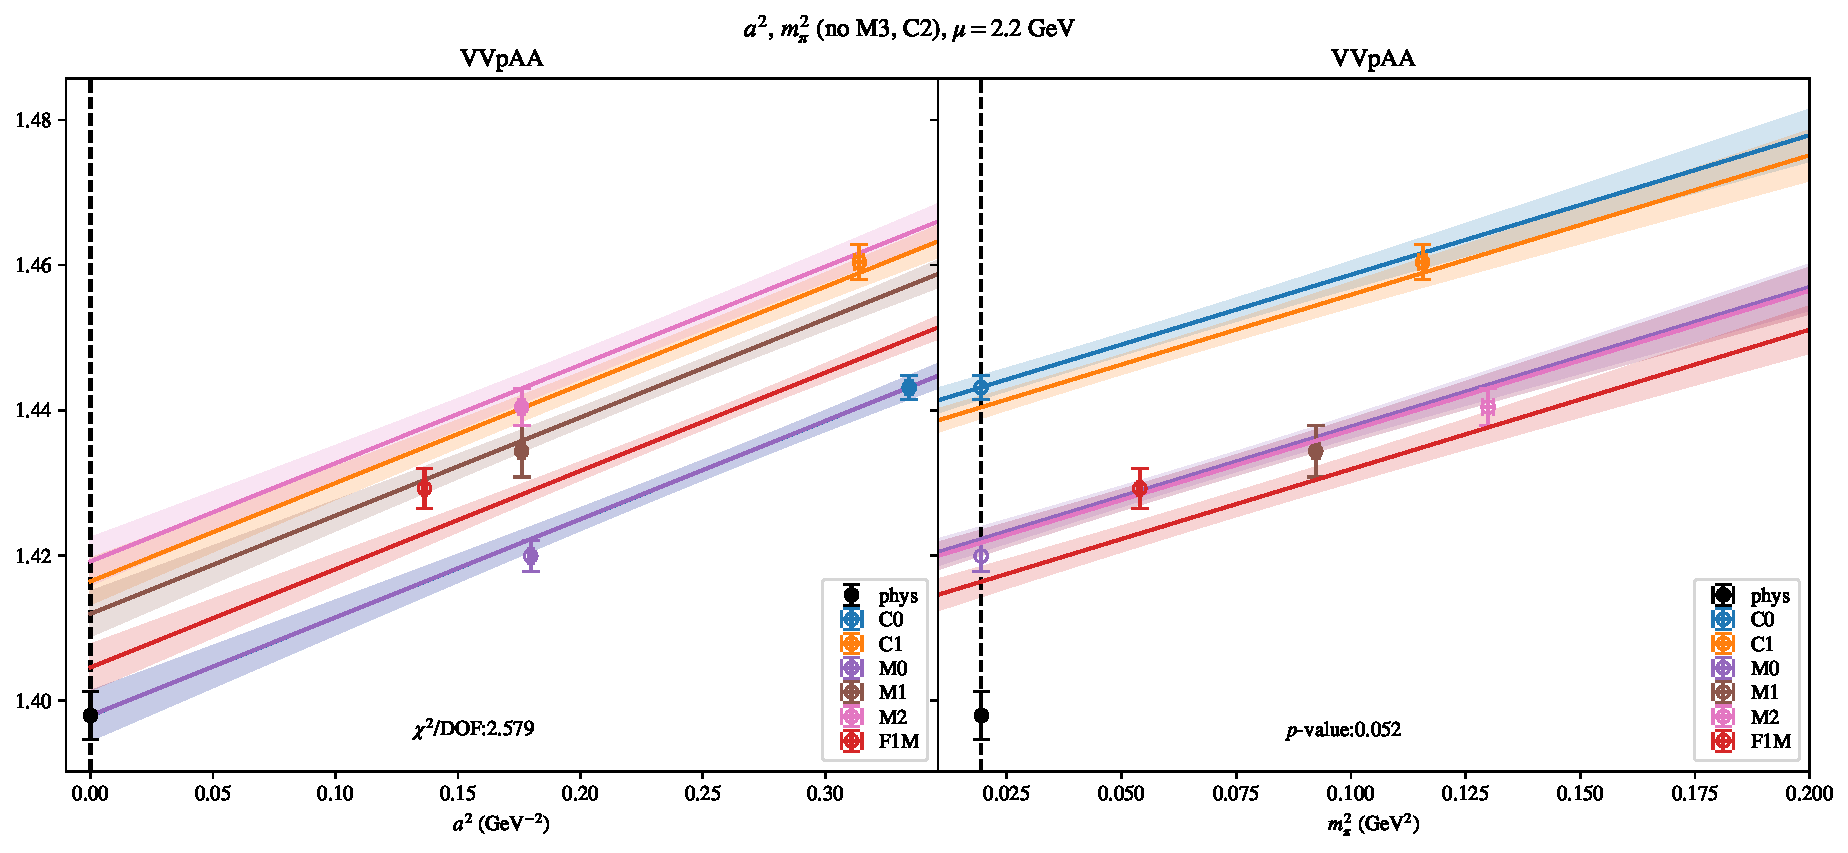
\includepdf[link, pages=-]{VVpAA/SUSY/bag_a2m2mcut_22.pdf}
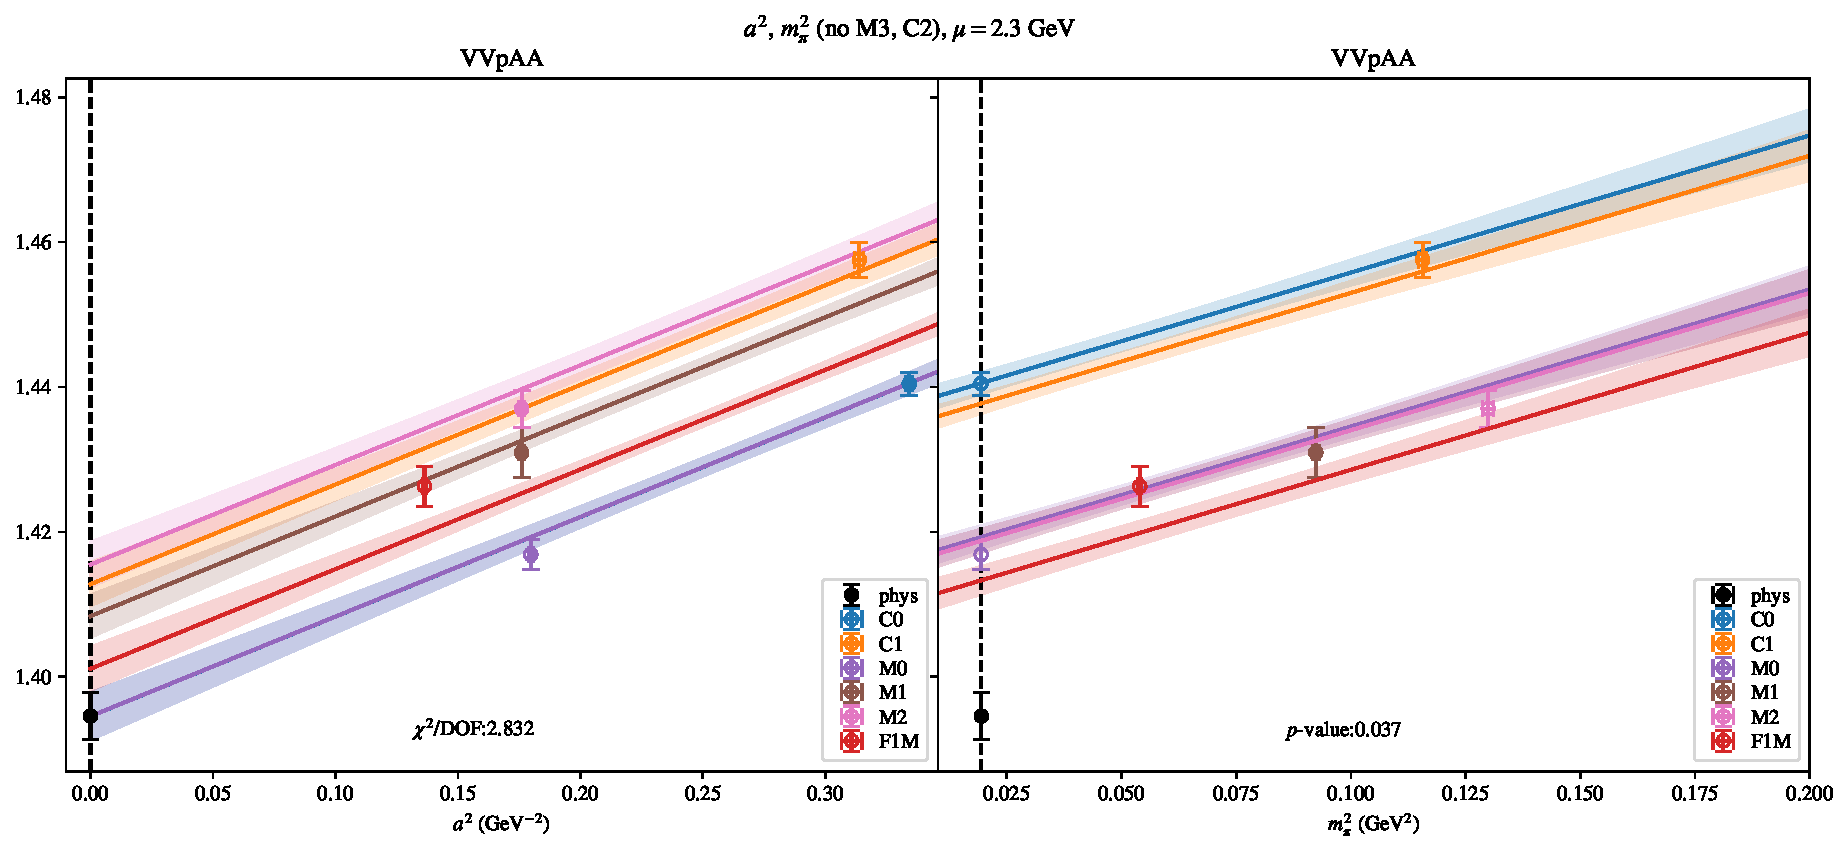
\includepdf[link, pages=-]{VVpAA/SUSY/bag_a2m2mcut_23.pdf}
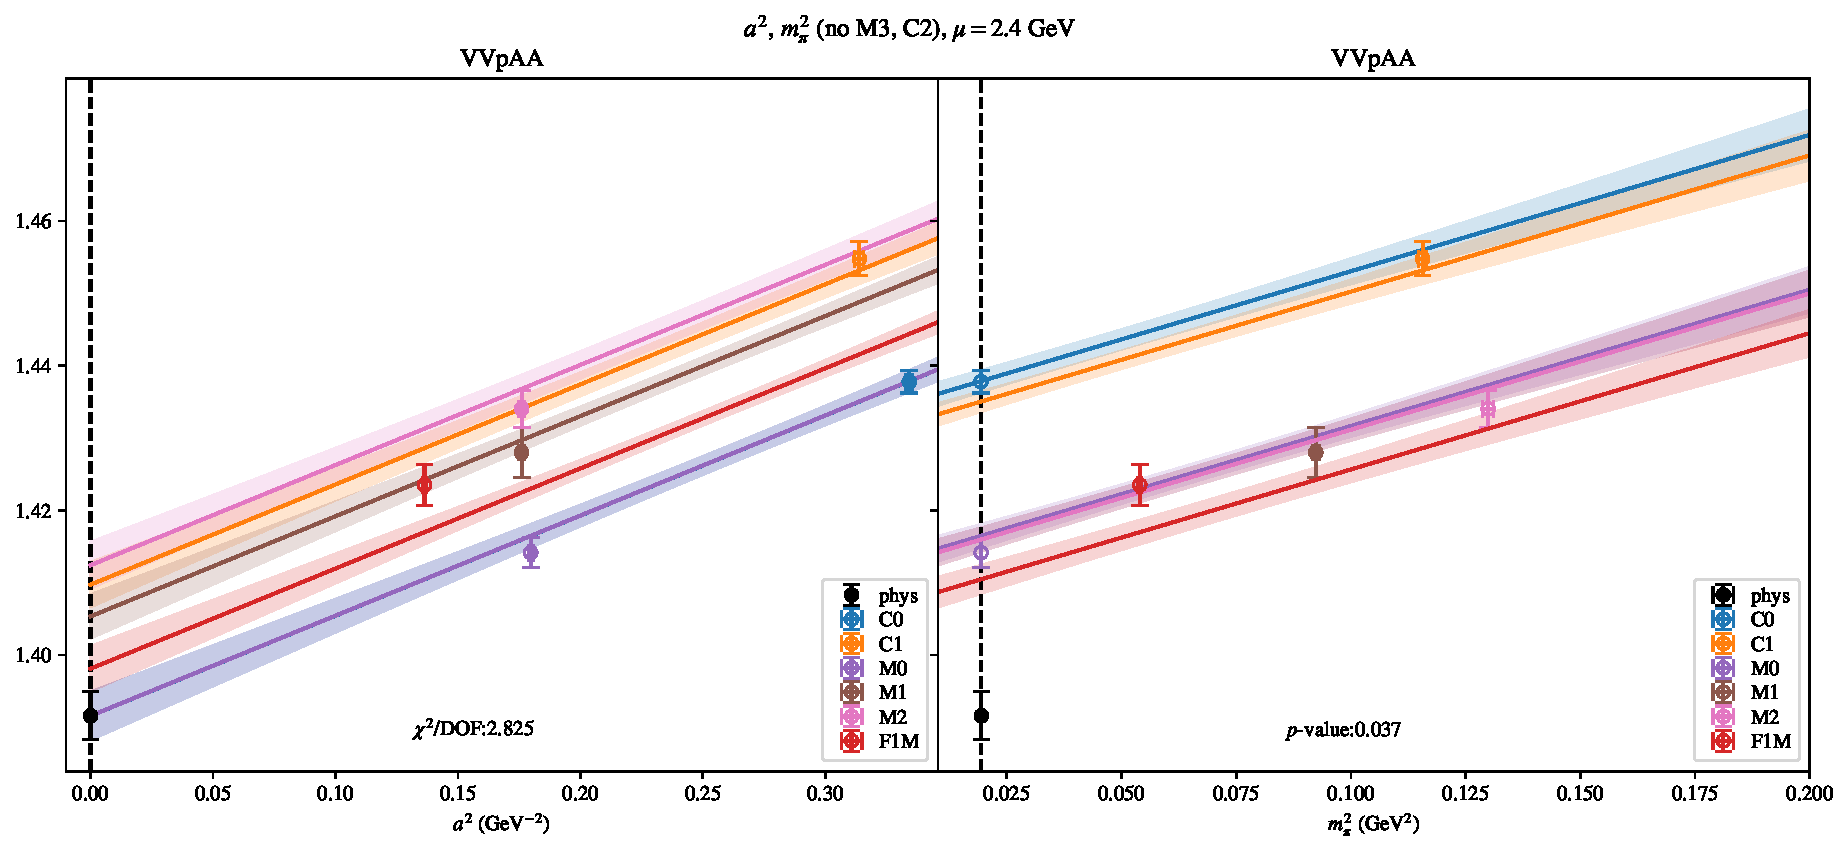
\includepdf[link, pages=-]{VVpAA/SUSY/bag_a2m2mcut_24.pdf}
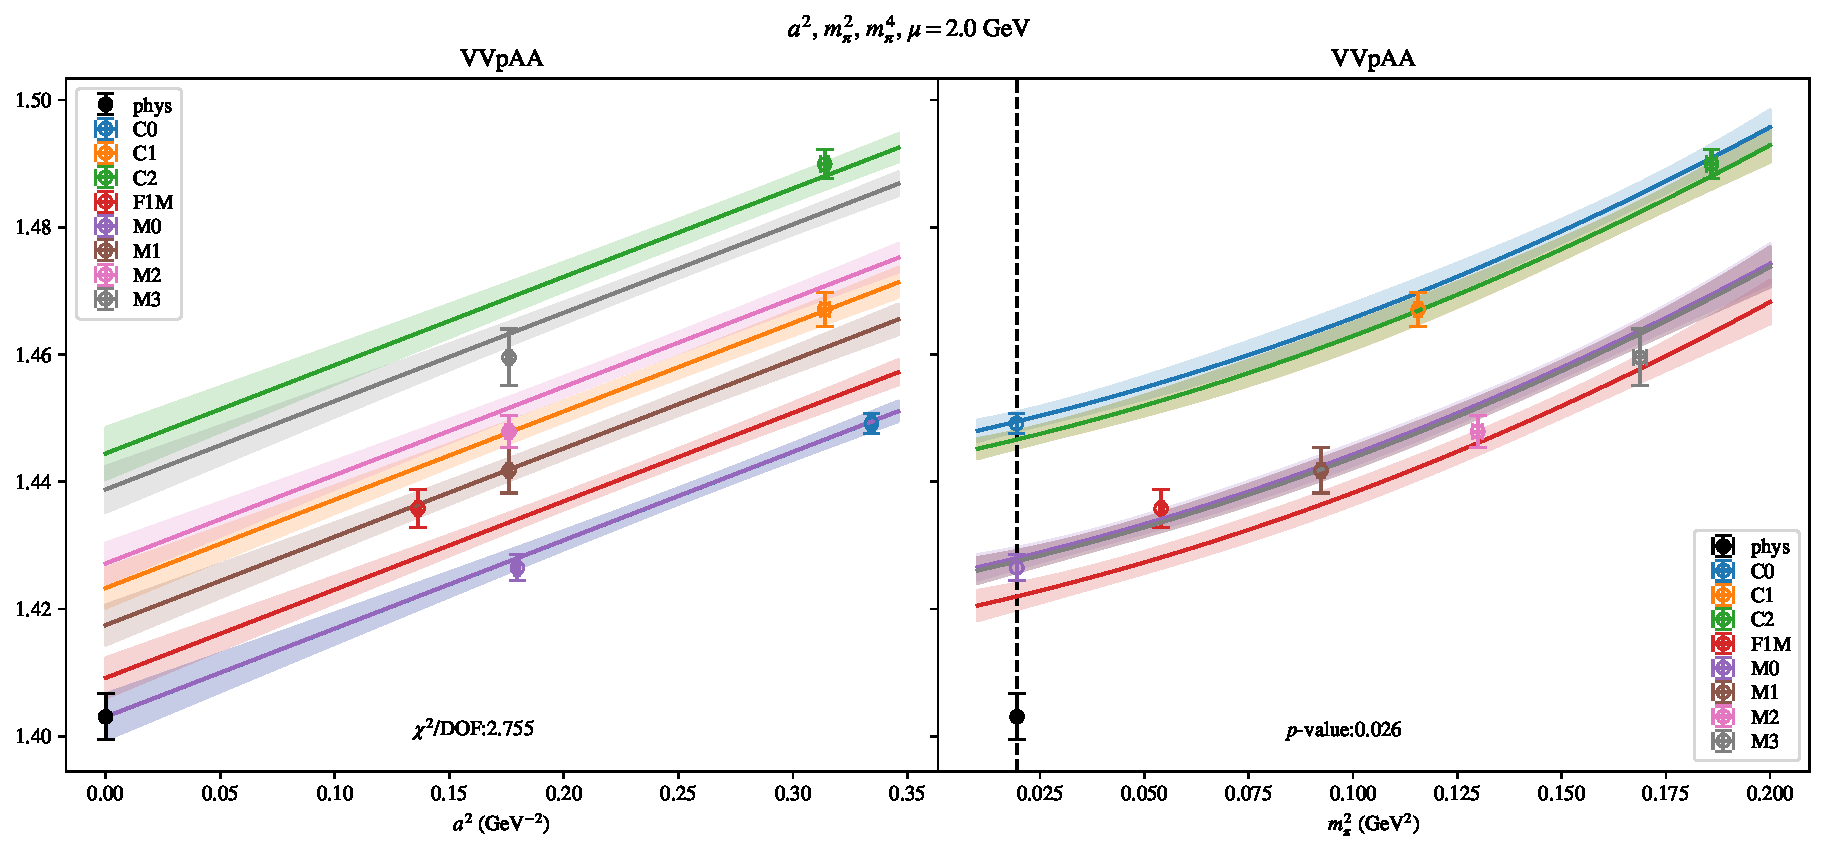
\includepdf[link, pages=-]{VVpAA/SUSY/bag_a2m2m4_20.pdf}
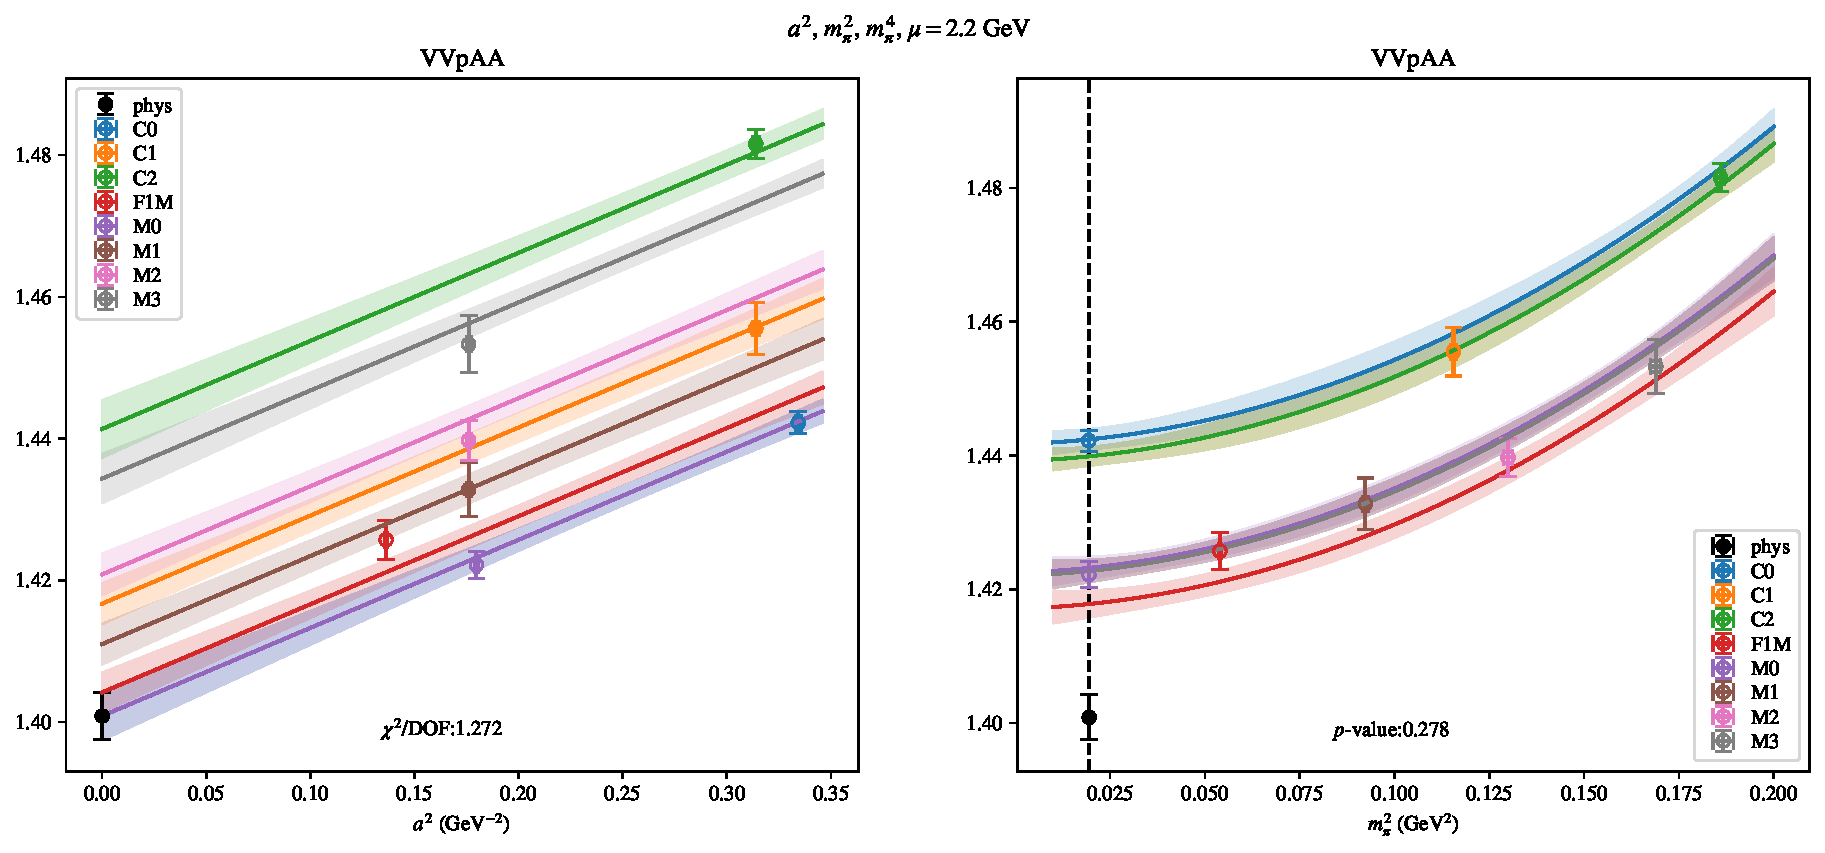
\includepdf[link, pages=-]{VVpAA/SUSY/bag_a2m2m4_22.pdf}
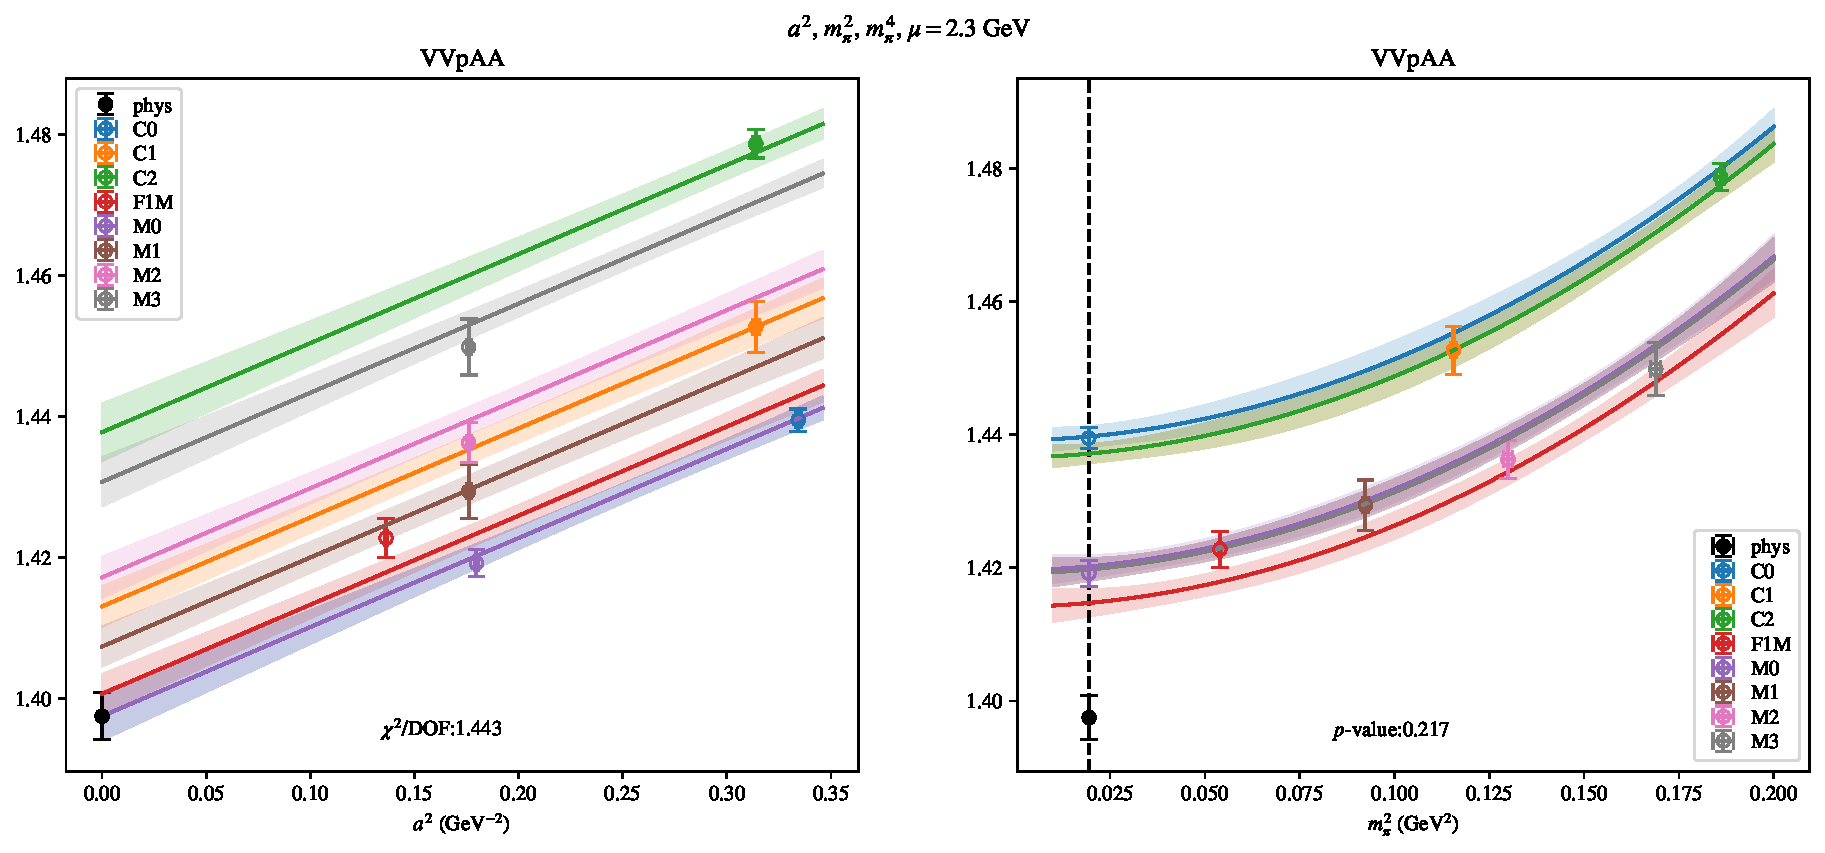
\includepdf[link, pages=-]{VVpAA/SUSY/bag_a2m2m4_23.pdf}
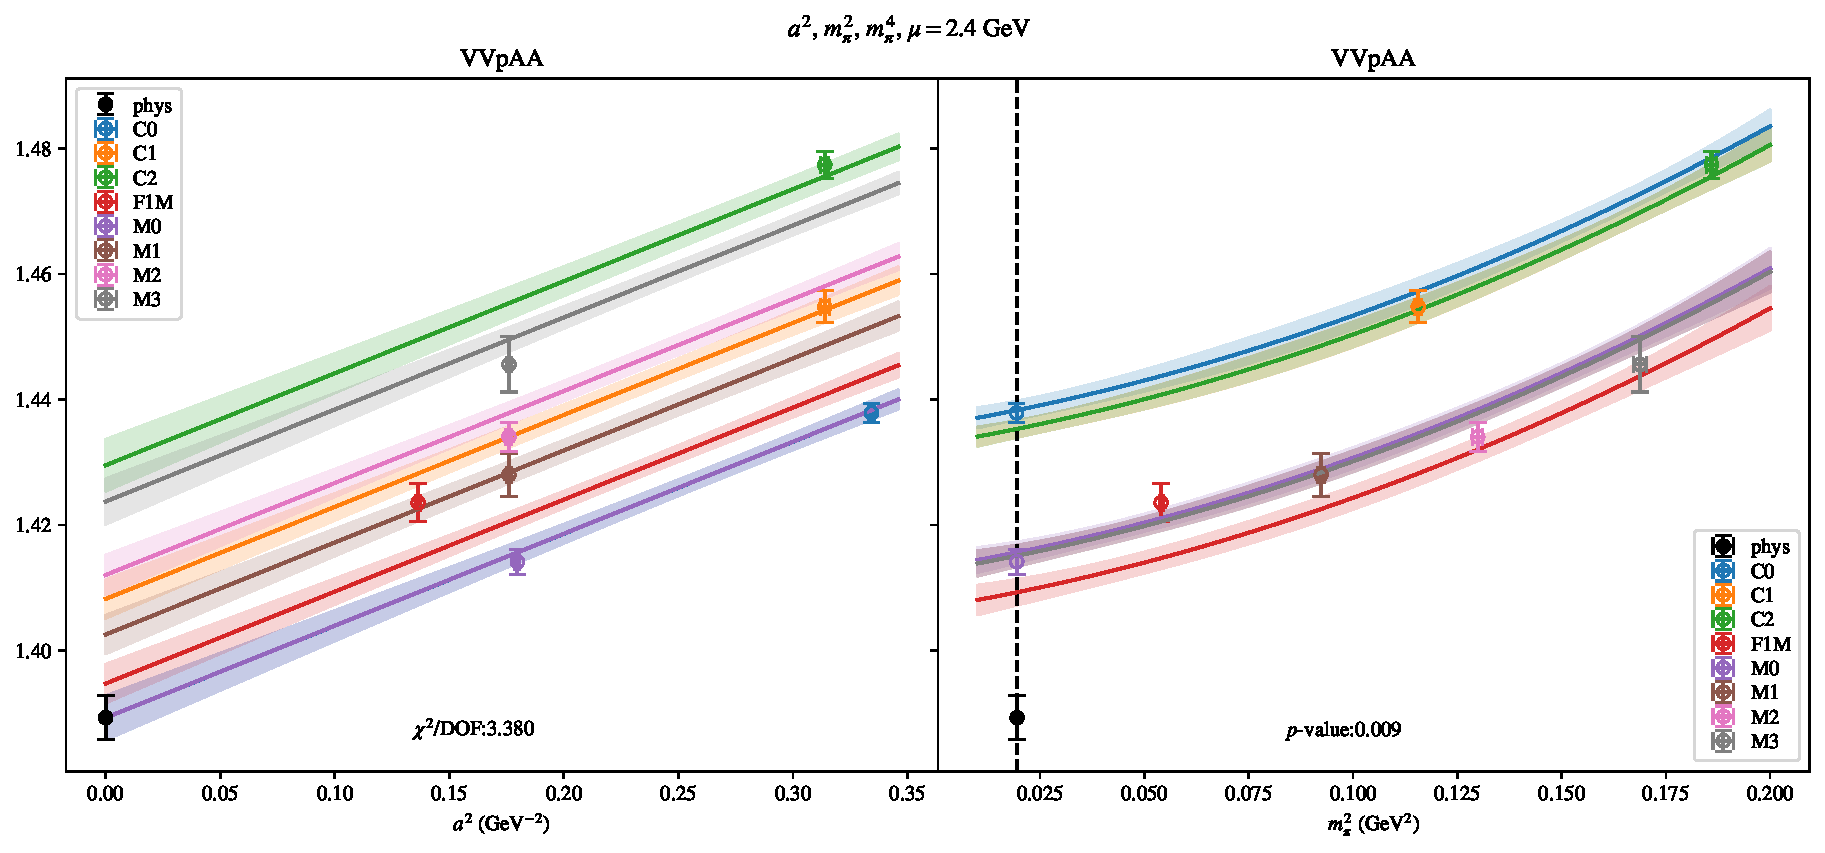
\includepdf[link, pages=-]{VVpAA/SUSY/bag_a2m2m4_24.pdf}
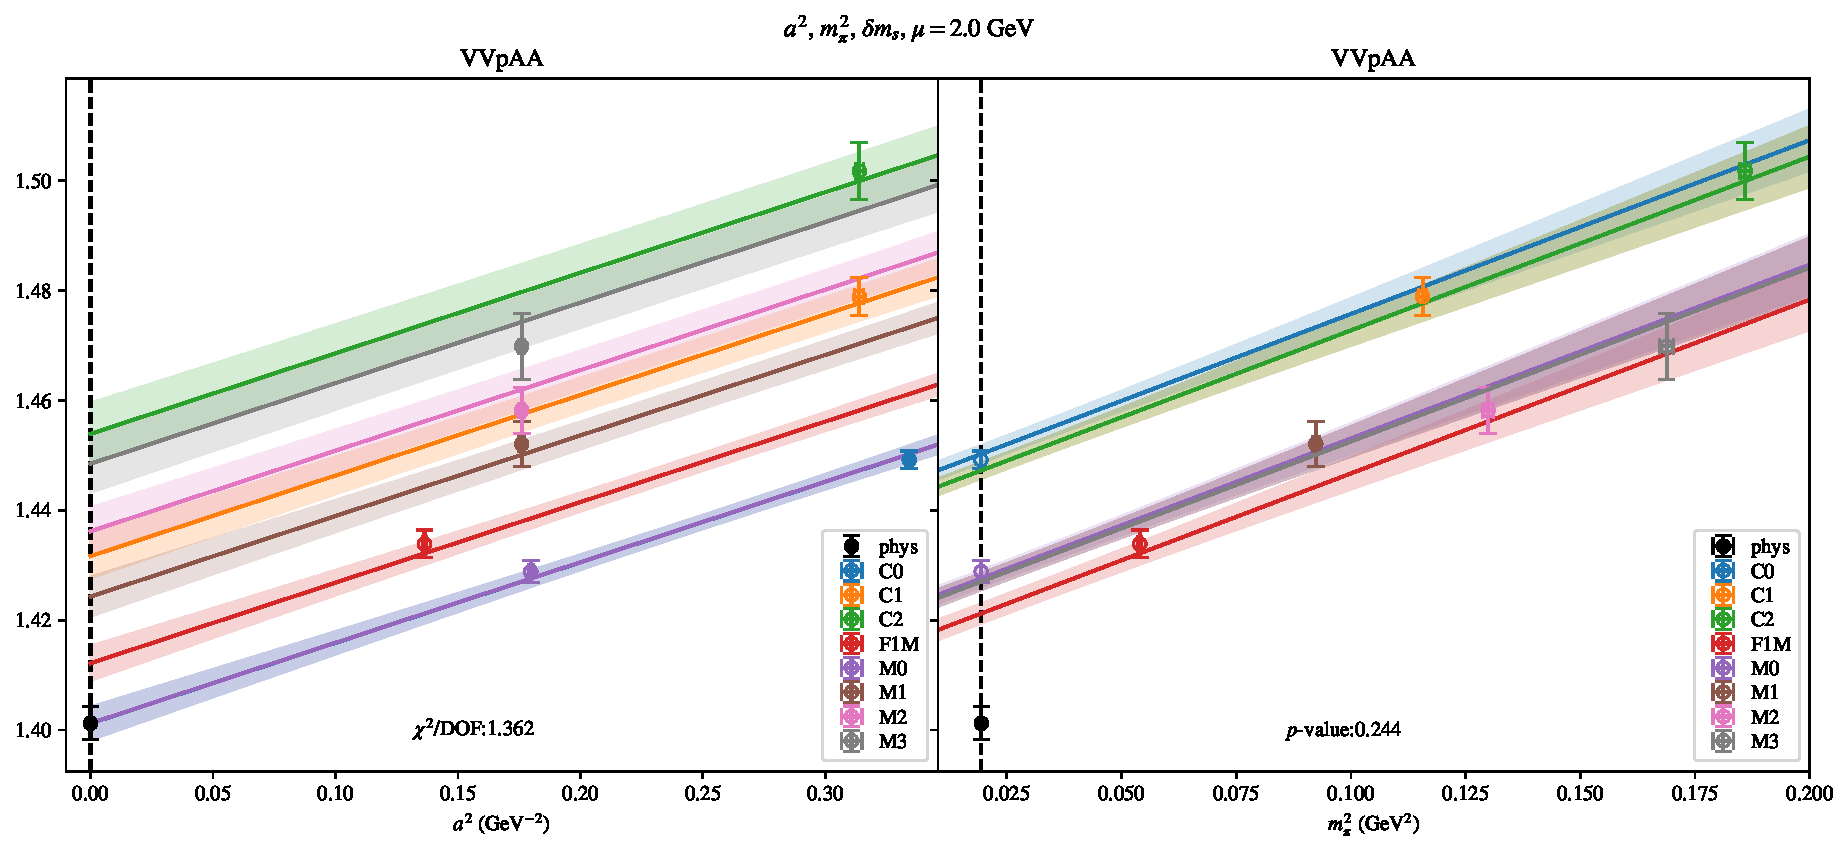
\includepdf[link, pages=-]{VVpAA/SUSY/bag_a2m2delm_20.pdf}
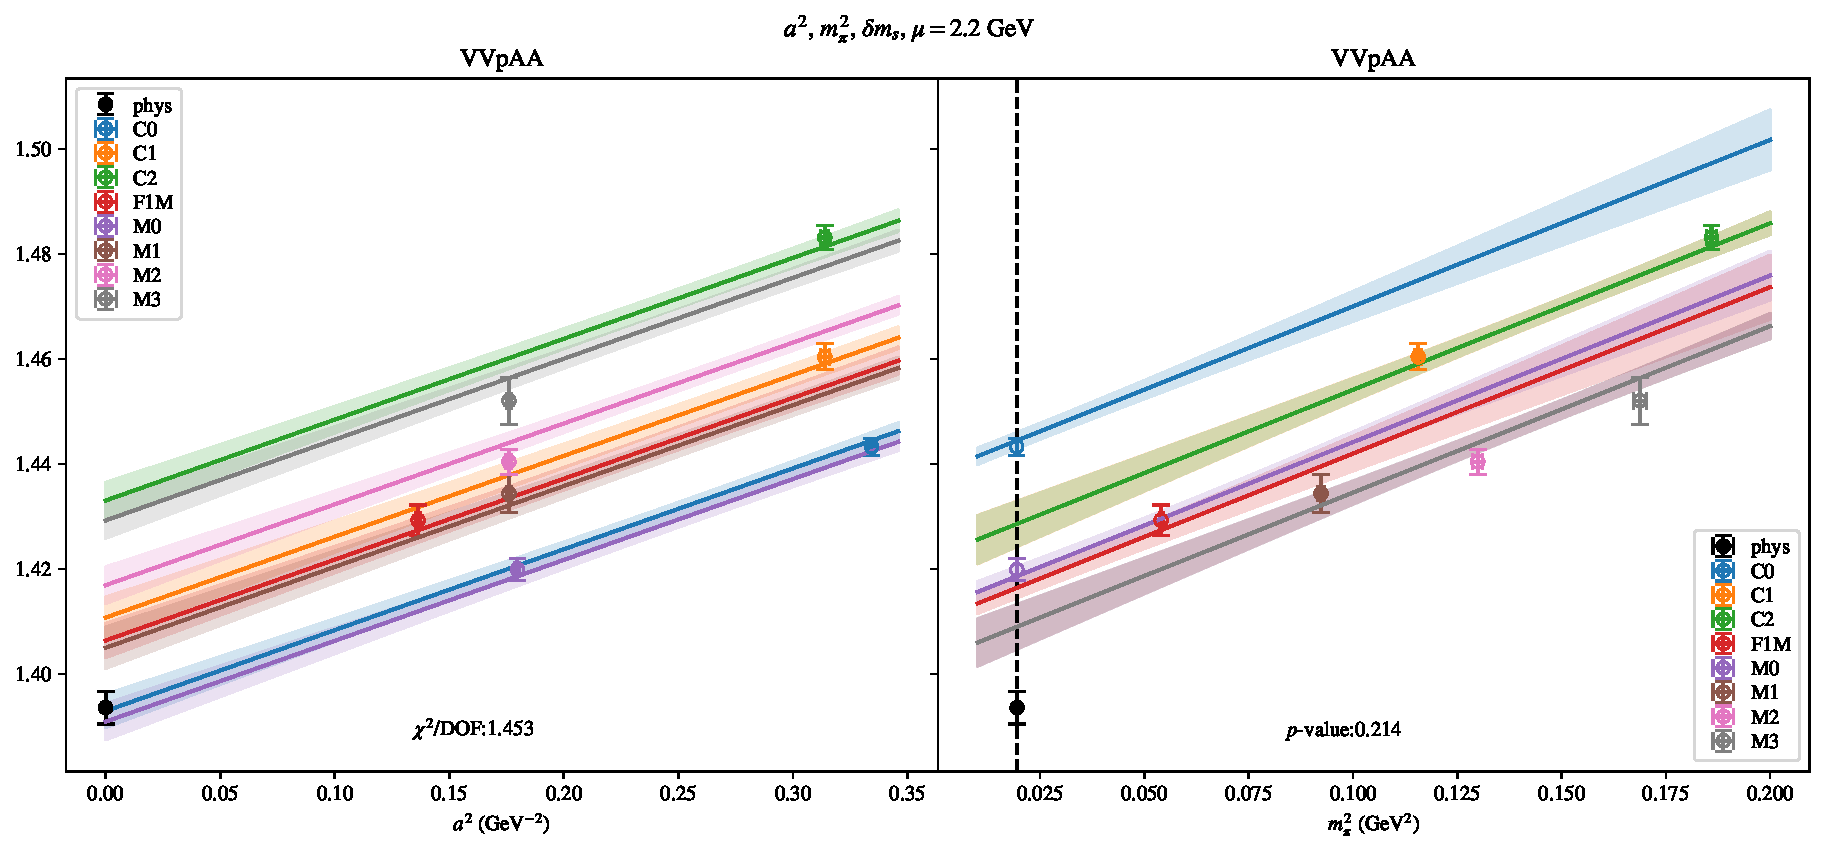
\includepdf[link, pages=-]{VVpAA/SUSY/bag_a2m2delm_22.pdf}
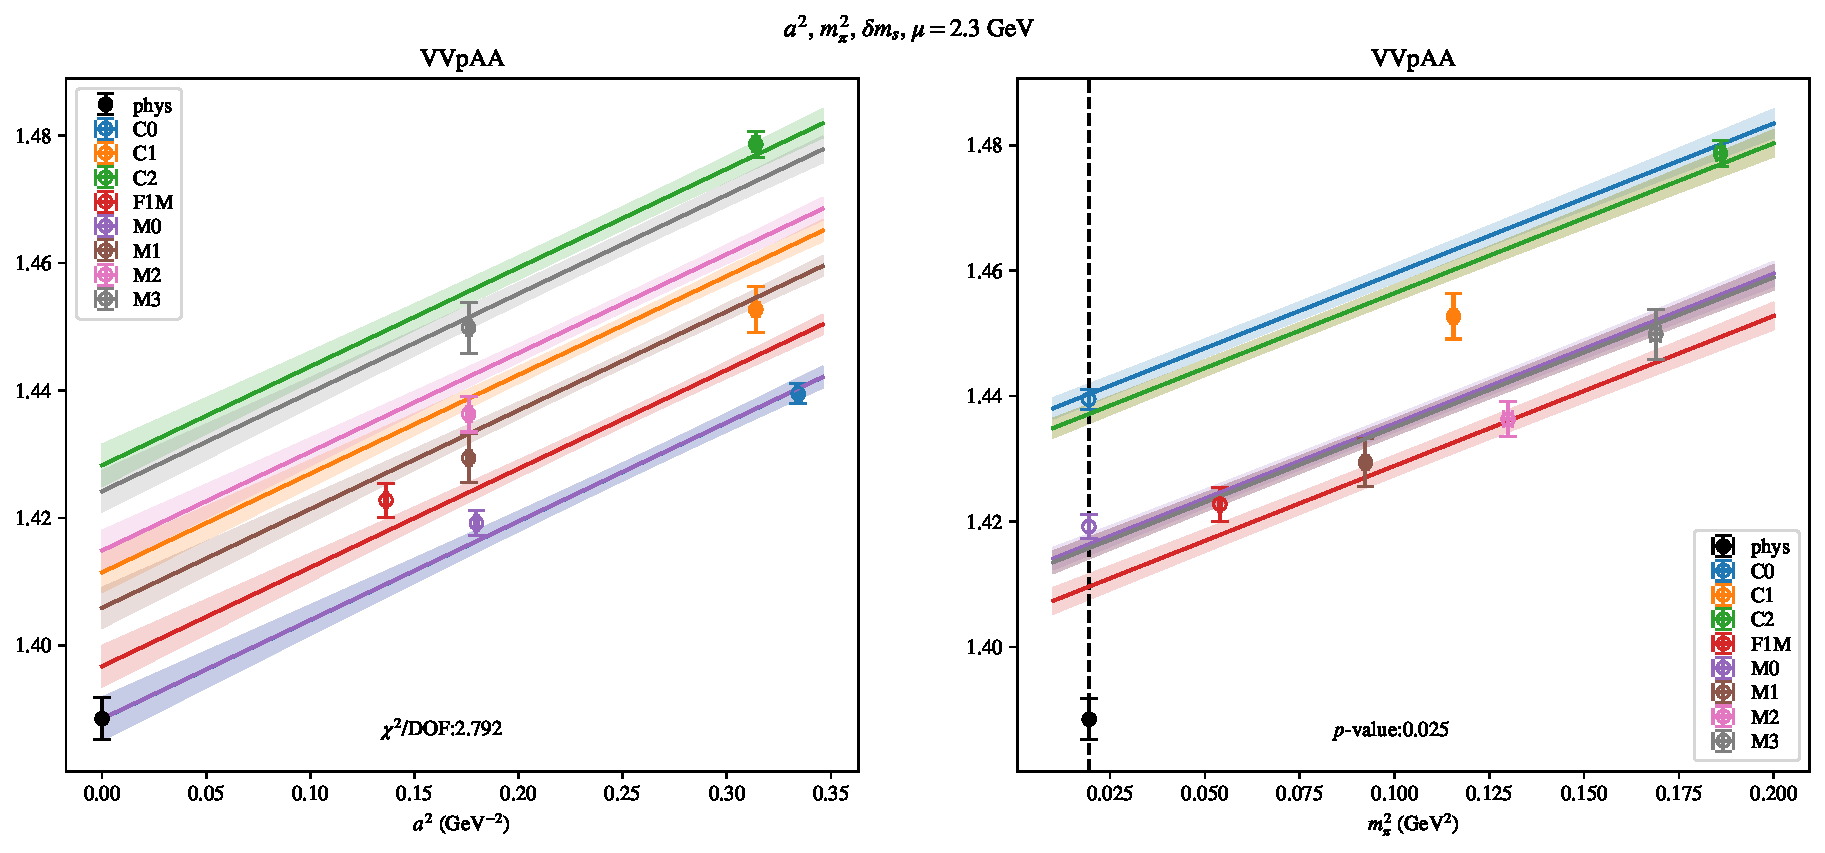
\includepdf[link, pages=-]{VVpAA/SUSY/bag_a2m2delm_23.pdf}
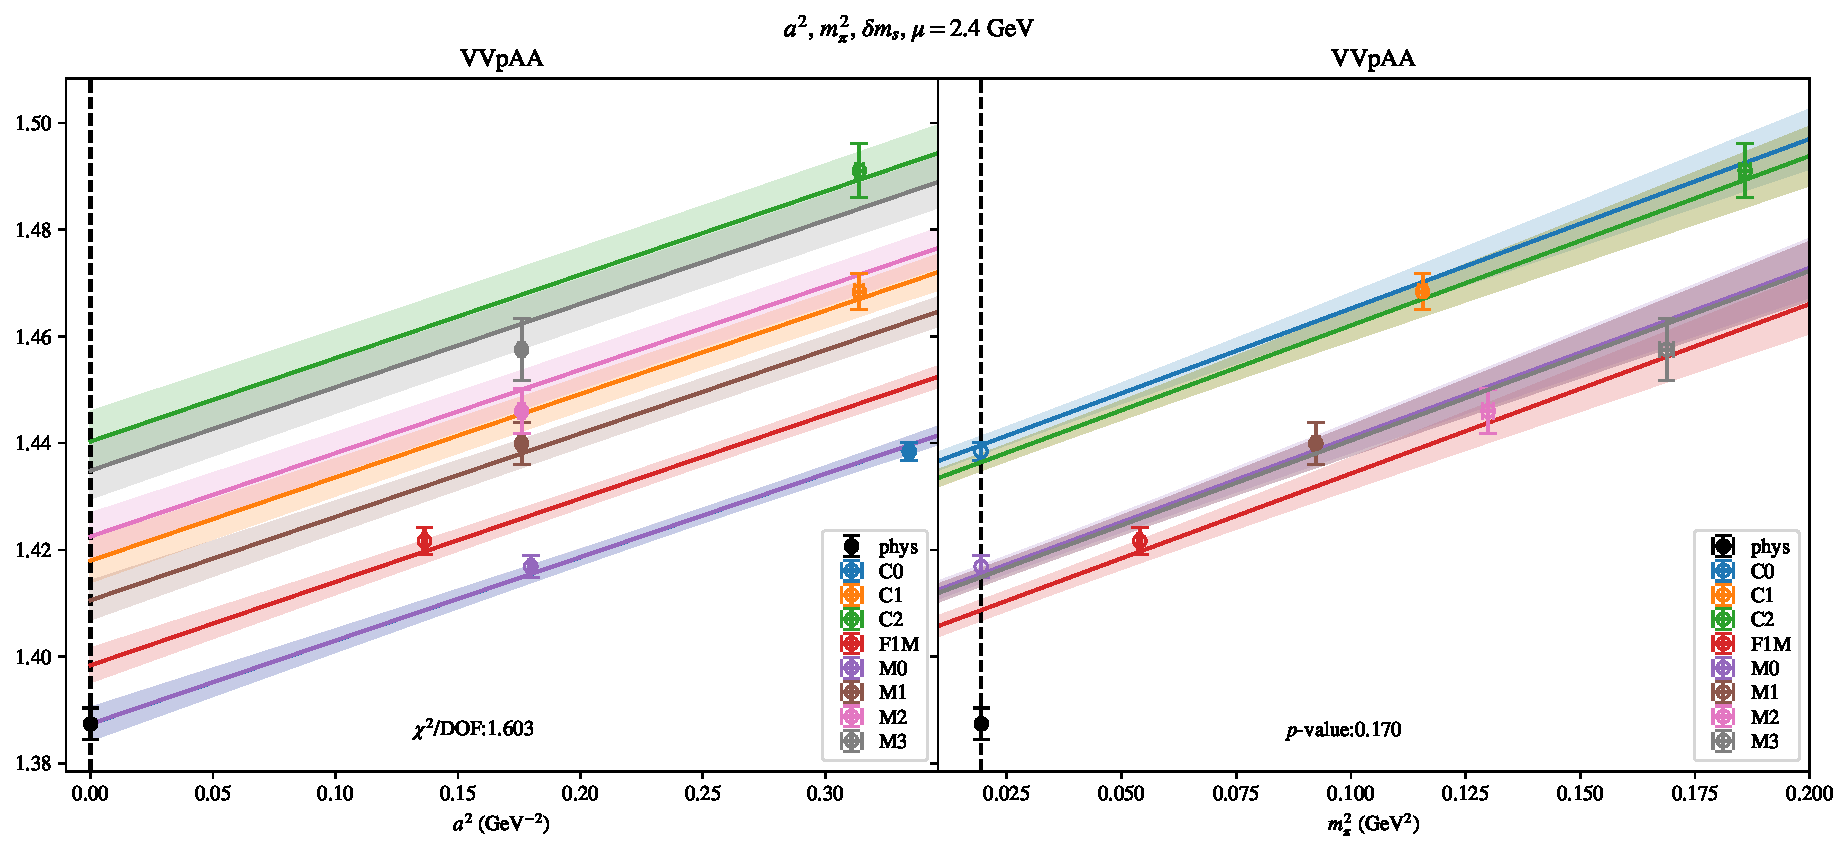
\includepdf[link, pages=-]{VVpAA/SUSY/bag_a2m2delm_24.pdf}
\clearpage
\section{$\mathcal{B}_2$}
\begin{table}[h!]
\begin{center}
\begin{tabular}{|c|c|c|c|c|c|c|}
\hline
$\mu$ (GeV) & $a^2$, $m_\pi^2$& $a^2$, $m_\pi^2$ (no C)& $a^2$, $m_\pi^2$, $a^4$& $a^2$, $m_\pi^2$ (no M3, C2)& $a^2$, $m_\pi^2$, $m_\pi^4$& $a^2$, $m_\pi^2$, $\delta m_s$\\
\hline
2.0& \hyperlink{VVmAA/SUSY/bag_a2m2_20.pdf.1}{\textbf{-0.9276(29)}: 0.836 (0.523)} & \hyperlink{VVmAA/SUSY/bag_a2m2noC_20.pdf.1}{\textbf{-0.940(13)}: 0.713 (0.49)} & \hyperlink{VVmAA/SUSY/bag_a2a4m2_20.pdf.1}{\textbf{-0.945(18)}: 0.923 (0.45)} & \hyperlink{VVmAA/SUSY/bag_a2m2mcut_20.pdf.1}{\textbf{-0.9268(28)}: 0.557 (0.644)} & \hyperlink{VVmAA/SUSY/bag_a2m2m4_20.pdf.1}{\textbf{-0.9256(30)}: 0.246 (0.912)} & \hyperlink{VVmAA/SUSY/bag_a2m2delm_20.pdf.1}{\textbf{-0.9277(27)}: 1.147 (0.332)}\\
2.2& \hyperlink{VVmAA/SUSY/bag_a2m2_22.pdf.1}{\textbf{-0.9078(22)}: 2.159 (0.056)} & \hyperlink{VVmAA/SUSY/bag_a2m2noC_22.pdf.1}{\textbf{-0.9273(98)}: 0.842 (0.431)} & \hyperlink{VVmAA/SUSY/bag_a2a4m2_22.pdf.1}{\textbf{-0.930(15)}: 2.09 (0.079)} & \hyperlink{VVmAA/SUSY/bag_a2m2mcut_22.pdf.1}{\textbf{-0.9071(19)}: 2.291 (0.076)} & \hyperlink{VVmAA/SUSY/bag_a2m2m4_22.pdf.1}{\textbf{-0.9056(21)}: 1.252 (0.287)} & \hyperlink{VVmAA/SUSY/bag_a2m2delm_22.pdf.1}{\textbf{-0.9078(21)}: 2.758 (0.026)}\\
2.3& \hyperlink{VVmAA/SUSY/bag_a2m2_23.pdf.1}{\textbf{-0.8986(20)}: 3.221 (0.007)} & \hyperlink{VVmAA/SUSY/bag_a2m2noC_23.pdf.1}{\textbf{-0.9205(87)}: 1.211 (0.298)} & \hyperlink{VVmAA/SUSY/bag_a2a4m2_23.pdf.1}{\textbf{-0.922(14)}: 3.523 (0.007)} & \hyperlink{VVmAA/SUSY/bag_a2m2mcut_23.pdf.1}{\textbf{-0.8985(19)}: 3.644 (0.012)} & \hyperlink{VVmAA/SUSY/bag_a2m2m4_23.pdf.1}{\textbf{-0.8963(21)}: 1.99 (0.093)} & \hyperlink{VVmAA/SUSY/bag_a2m2delm_23.pdf.1}{\textbf{-0.8988(19)}: 4.175 (0.002)}\\
2.4& \hyperlink{VVmAA/SUSY/bag_a2m2_24.pdf.1}{\textbf{-0.8908(19)}: 3.894 (0.002)} & \hyperlink{VVmAA/SUSY/bag_a2m2noC_24.pdf.1}{\textbf{-0.9135(83)}: 1.28 (0.278)} & \hyperlink{VVmAA/SUSY/bag_a2a4m2_24.pdf.1}{\textbf{-0.915(14)}: 3.85 (0.004)} & \hyperlink{VVmAA/SUSY/bag_a2m2mcut_24.pdf.1}{\textbf{-0.8901(18)}: 4.259 (0.005)} & \hyperlink{VVmAA/SUSY/bag_a2m2m4_24.pdf.1}{\textbf{-0.8882(19)}: 2.66 (0.031)} & \hyperlink{VVmAA/SUSY/bag_a2m2delm_24.pdf.1}{\textbf{-0.8907(19)}: 4.708 (0.001)}\\
\hline
\end{tabular}
\caption{Physical point value from chiral and continuum extrapolation at renormalisation scale $\mu$. Entries are \textbf{value(error)}: $\chi^2/\text{DOF}$ ($p$-value).}
\end{center}
\end{table}
\begin{table}[h!]
\begin{center}
\begin{tabular}{|c c|c|c|c|c|c|c|}
\hline
$\mu$ (GeV) &  & $a^2$, $m_\pi^2$& $a^2$, $m_\pi^2$ (no C)& $a^2$, $m_\pi^2$, $a^4$& $a^2$, $m_\pi^2$ (no M3, C2)& $a^2$, $m_\pi^2$, $m_\pi^4$& $a^2$, $m_\pi^2$, $\delta m_s$\\
\hline
\multirow{3}{0.5in}{2.0} & $\alpha$ & -0.345(10)& -0.271(77)& -0.19(16)& -0.347(10)& -0.351(10)& -0.345(10)\\
 & $\beta$ & -0.00707(32)& -0.00699(67)& -0.00709(28)& -0.00770(45)& -0.00959(97)& -0.00711(48)\\
 & $\gamma$ &  &  & -0.32(33)&  & 0.000235(80)& 0.002(21)\\
\hline
\multirow{3}{0.5in}{2.2} & $\alpha$ & -0.3777(84)& -0.265(57)& -0.18(14)& -0.3797(73)& -0.3847(79)& -0.3784(85)\\
 & $\beta$ & -0.00682(17)& -0.00643(46)& -0.00690(19)& -0.00729(30)& -0.00911(79)& -0.00694(36)\\
 & $\gamma$ &  &  & -0.40(29)&  & 0.000211(67)& 0.005(15)\\
\hline
\multirow{3}{0.5in}{2.3} & $\alpha$ & -0.3958(77)& -0.270(50)& -0.19(13)& -0.3955(73)& -0.4028(78)& -0.3954(75)\\
 & $\beta$ & -0.00688(18)& -0.00641(35)& -0.00696(18)& -0.00732(30)& -0.00928(76)& -0.00700(34)\\
 & $\gamma$ &  &  & -0.42(26)&  & 0.000222(65)& 0.006(14)\\
\hline
\multirow{3}{0.5in}{2.4} & $\alpha$ & -0.4098(75)& -0.279(48)& -0.19(13)& -0.4114(69)& -0.4178(70)& -0.4102(80)\\
 & $\beta$ & -0.00685(18)& -0.00638(36)& -0.00692(17)& -0.00732(29)& -0.00928(75)& -0.00694(35)\\
 & $\gamma$ &  &  & -0.44(27)&  & 0.000220(65)& 0.004(15)\\
\hline
\end{tabular}
\caption{Fit values of coefficients in $Q = Q_{phys} + \mathbf{\alpha} a^2 + \mathbf{\beta}\left(\frac{m_\pi^2}{f_\pi^2}-\frac{m_{\pi,PDG}^2}{f_\pi^2}\right) + \gamma(\ldots)$}
\end{center}
\end{table}
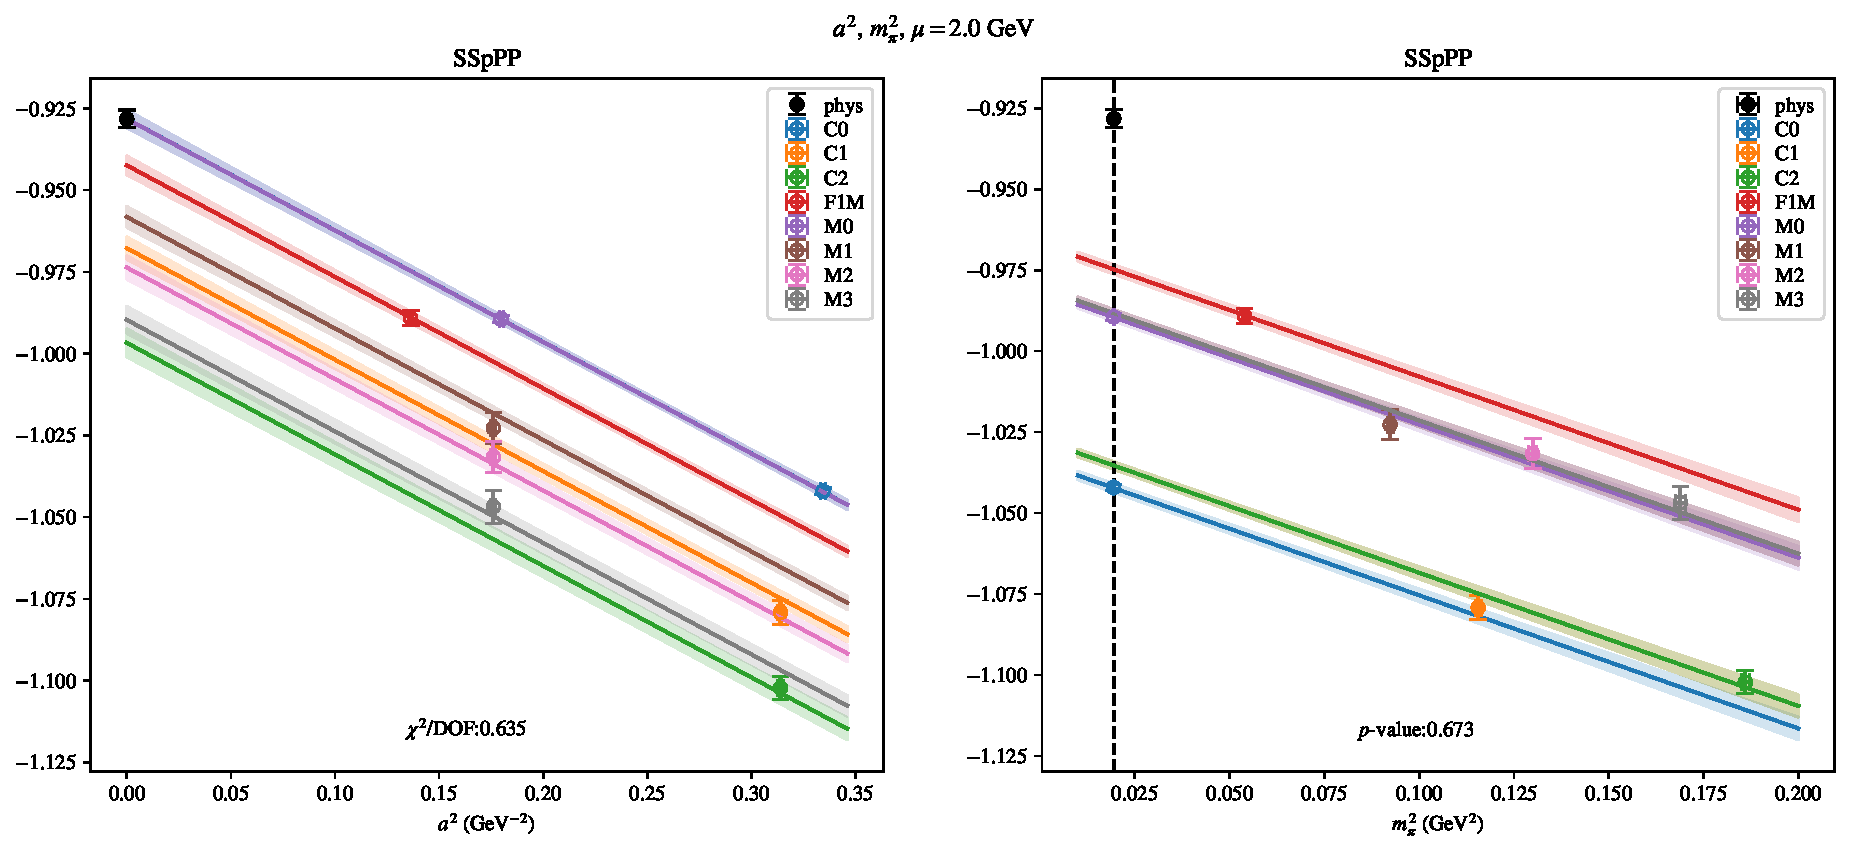
\includepdf[link, pages=-]{VVmAA/SUSY/bag_a2m2_20.pdf}
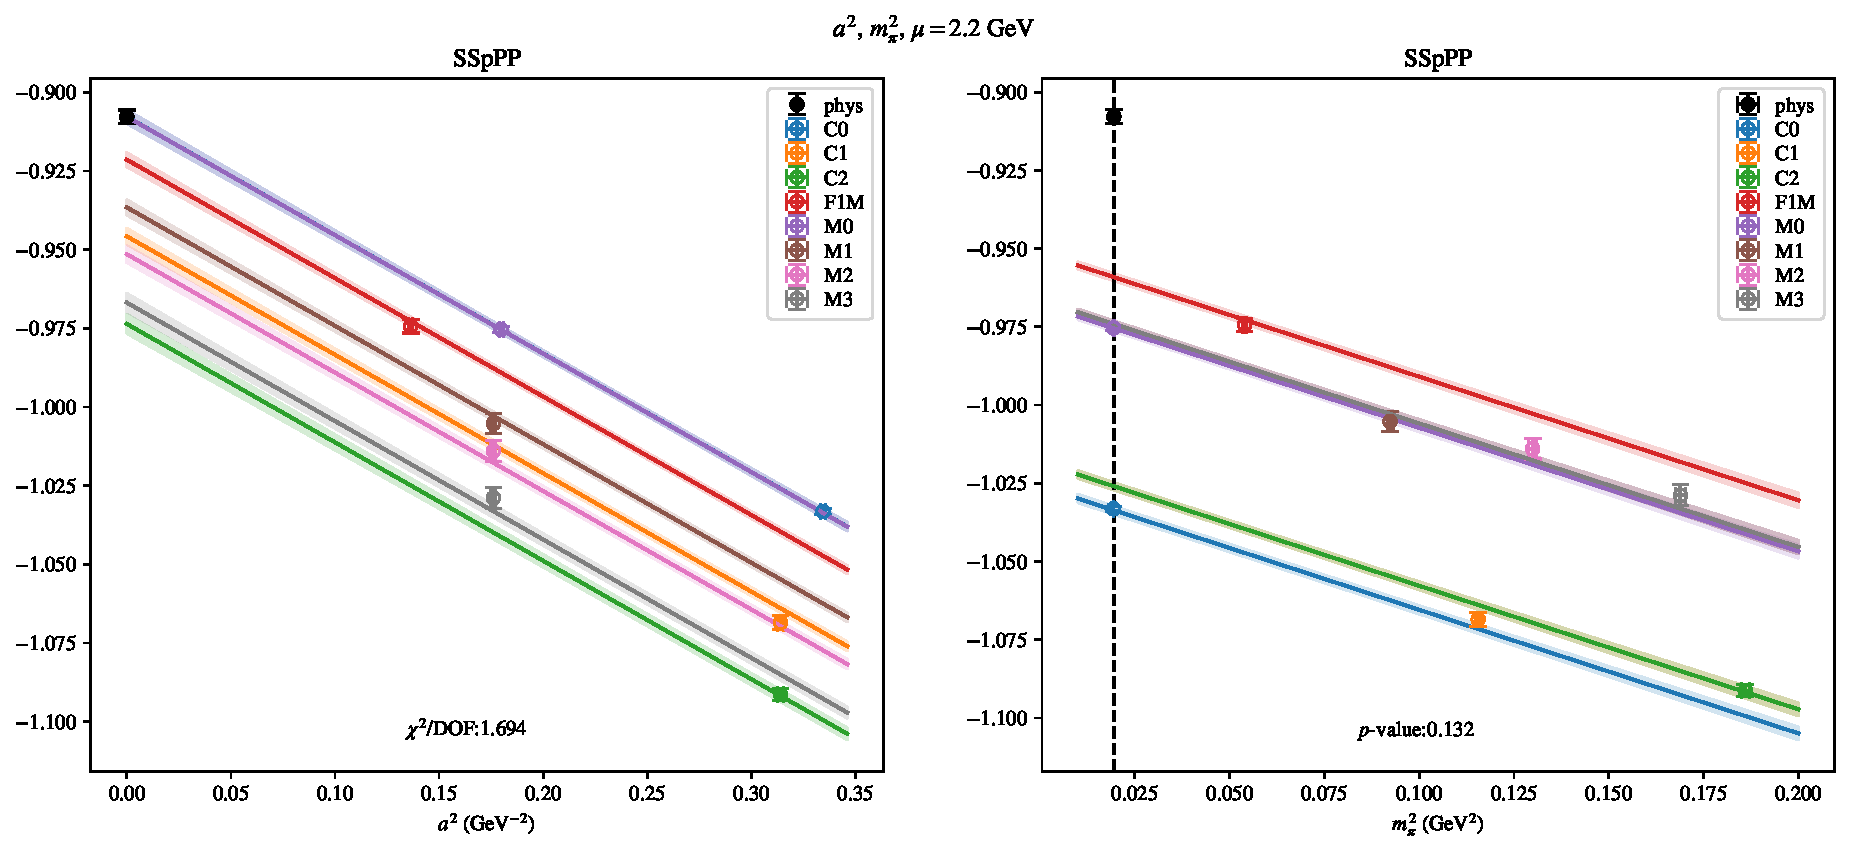
\includepdf[link, pages=-]{VVmAA/SUSY/bag_a2m2_22.pdf}
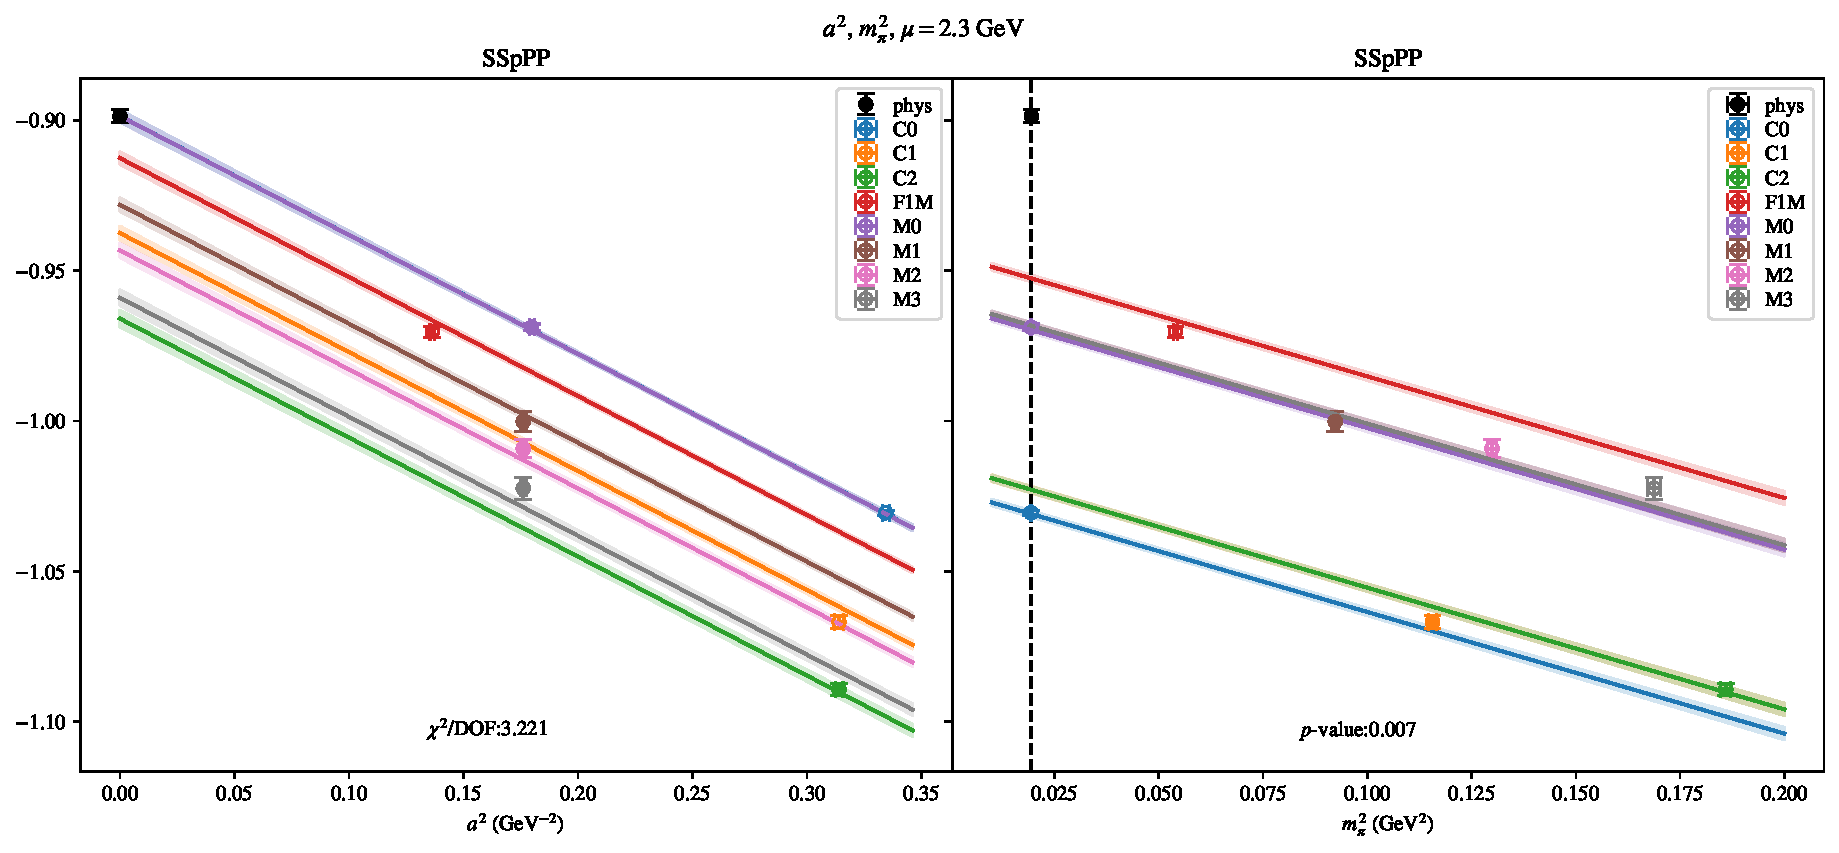
\includepdf[link, pages=-]{VVmAA/SUSY/bag_a2m2_23.pdf}
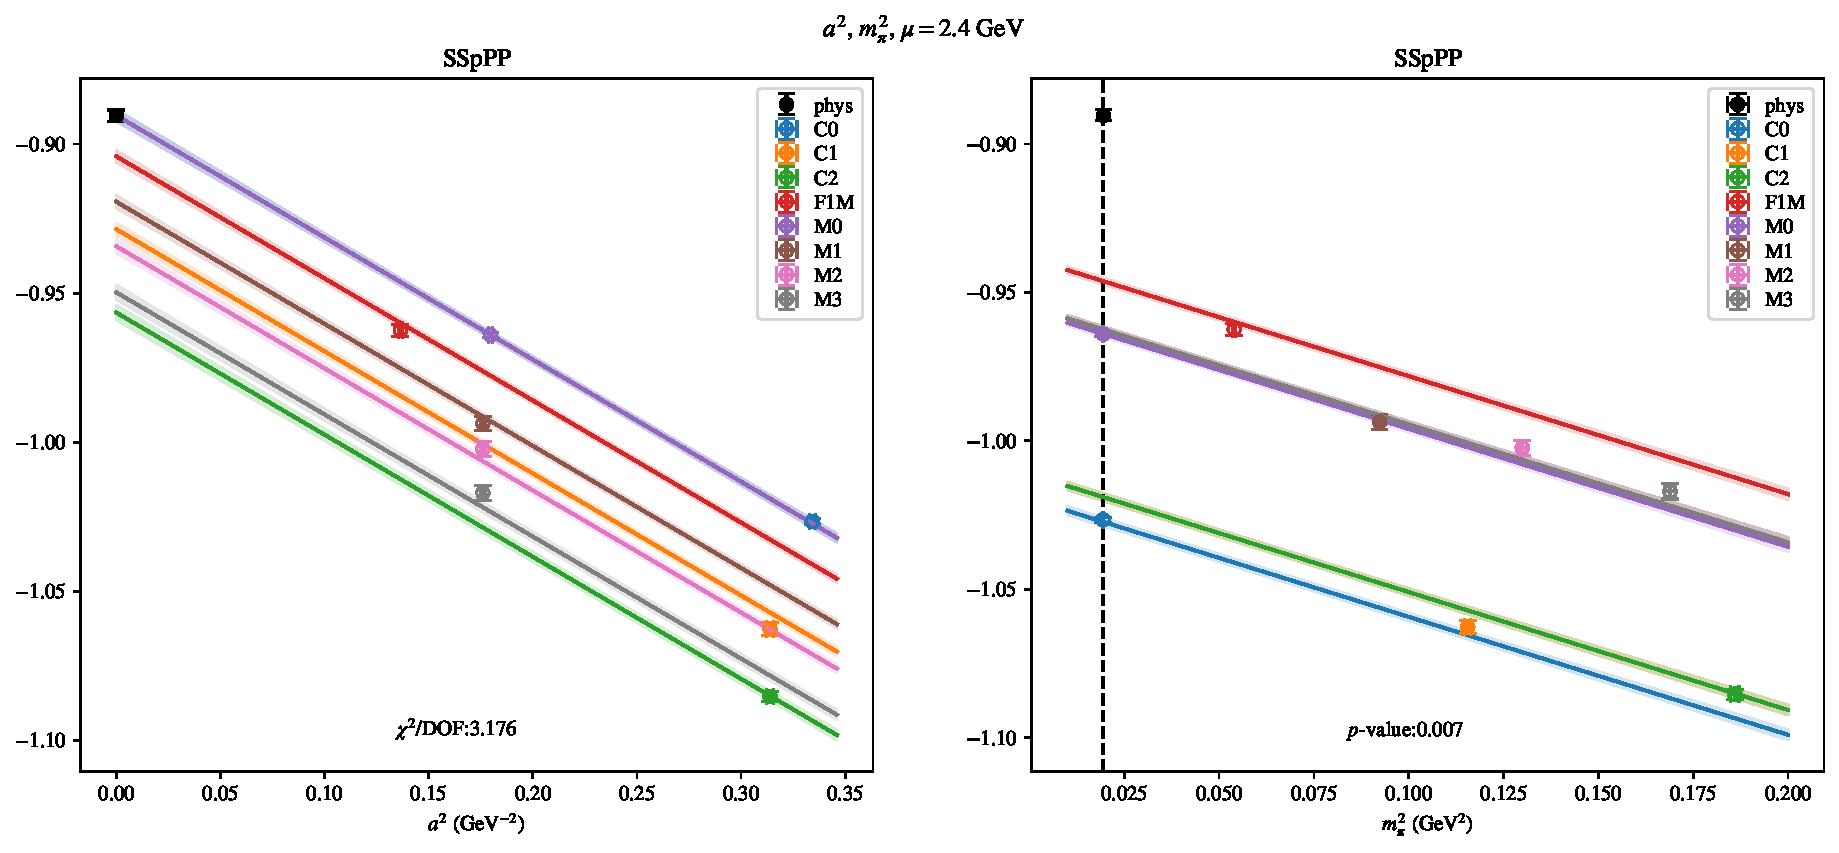
\includepdf[link, pages=-]{VVmAA/SUSY/bag_a2m2_24.pdf}
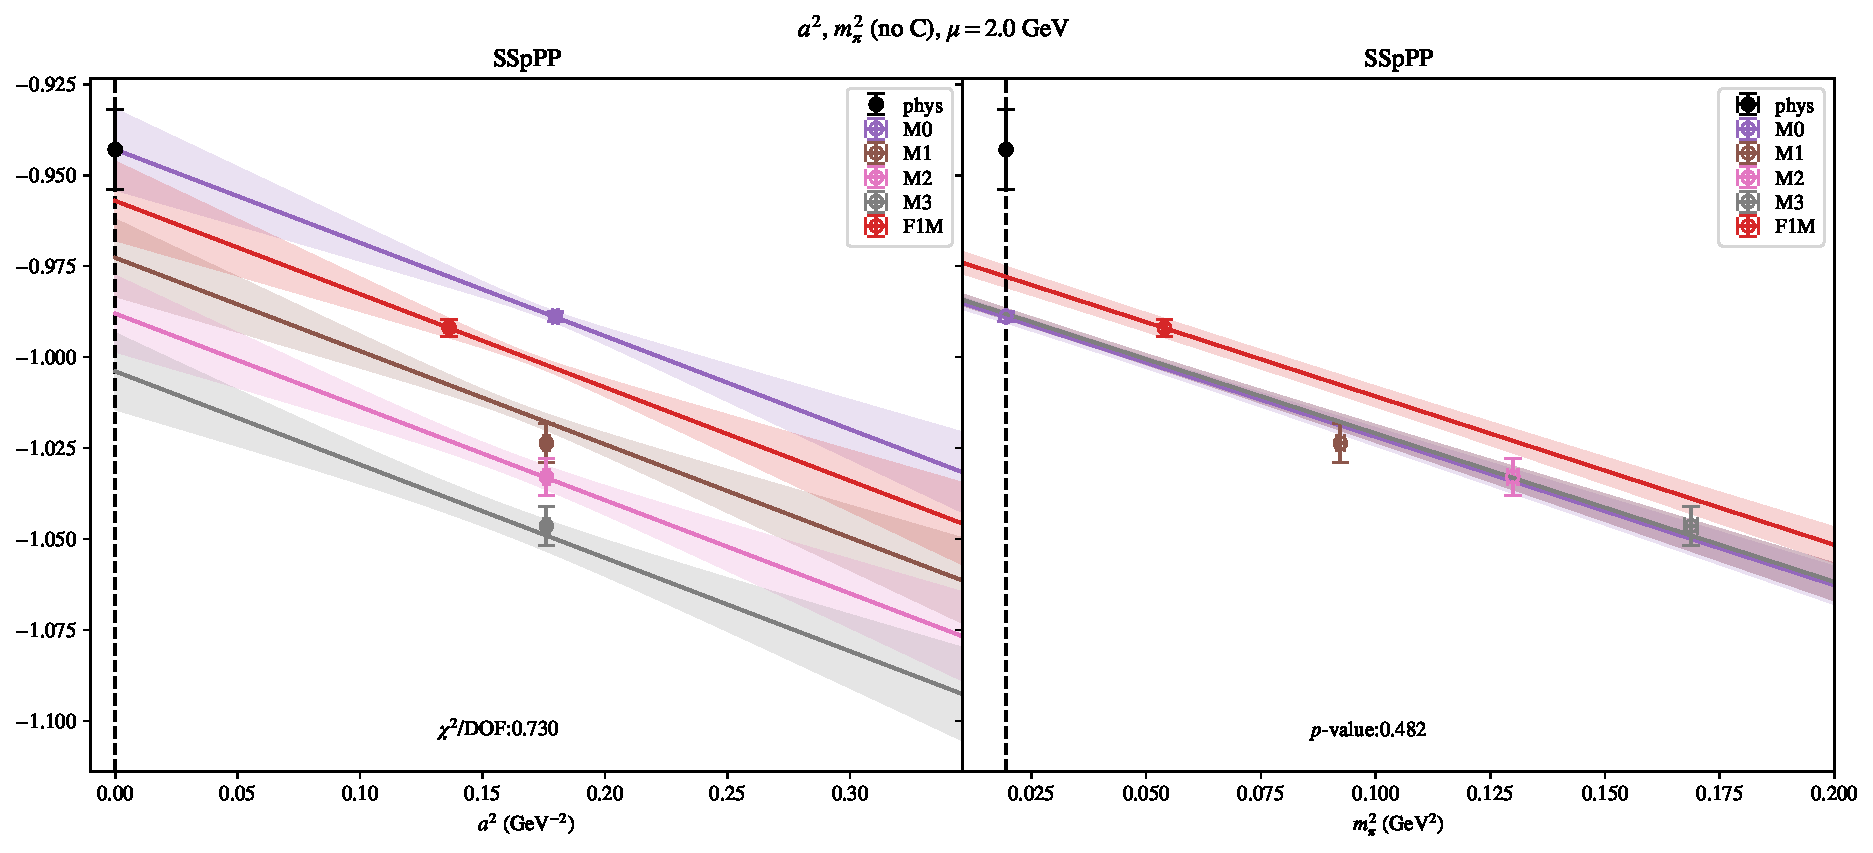
\includepdf[link, pages=-]{VVmAA/SUSY/bag_a2m2noC_20.pdf}
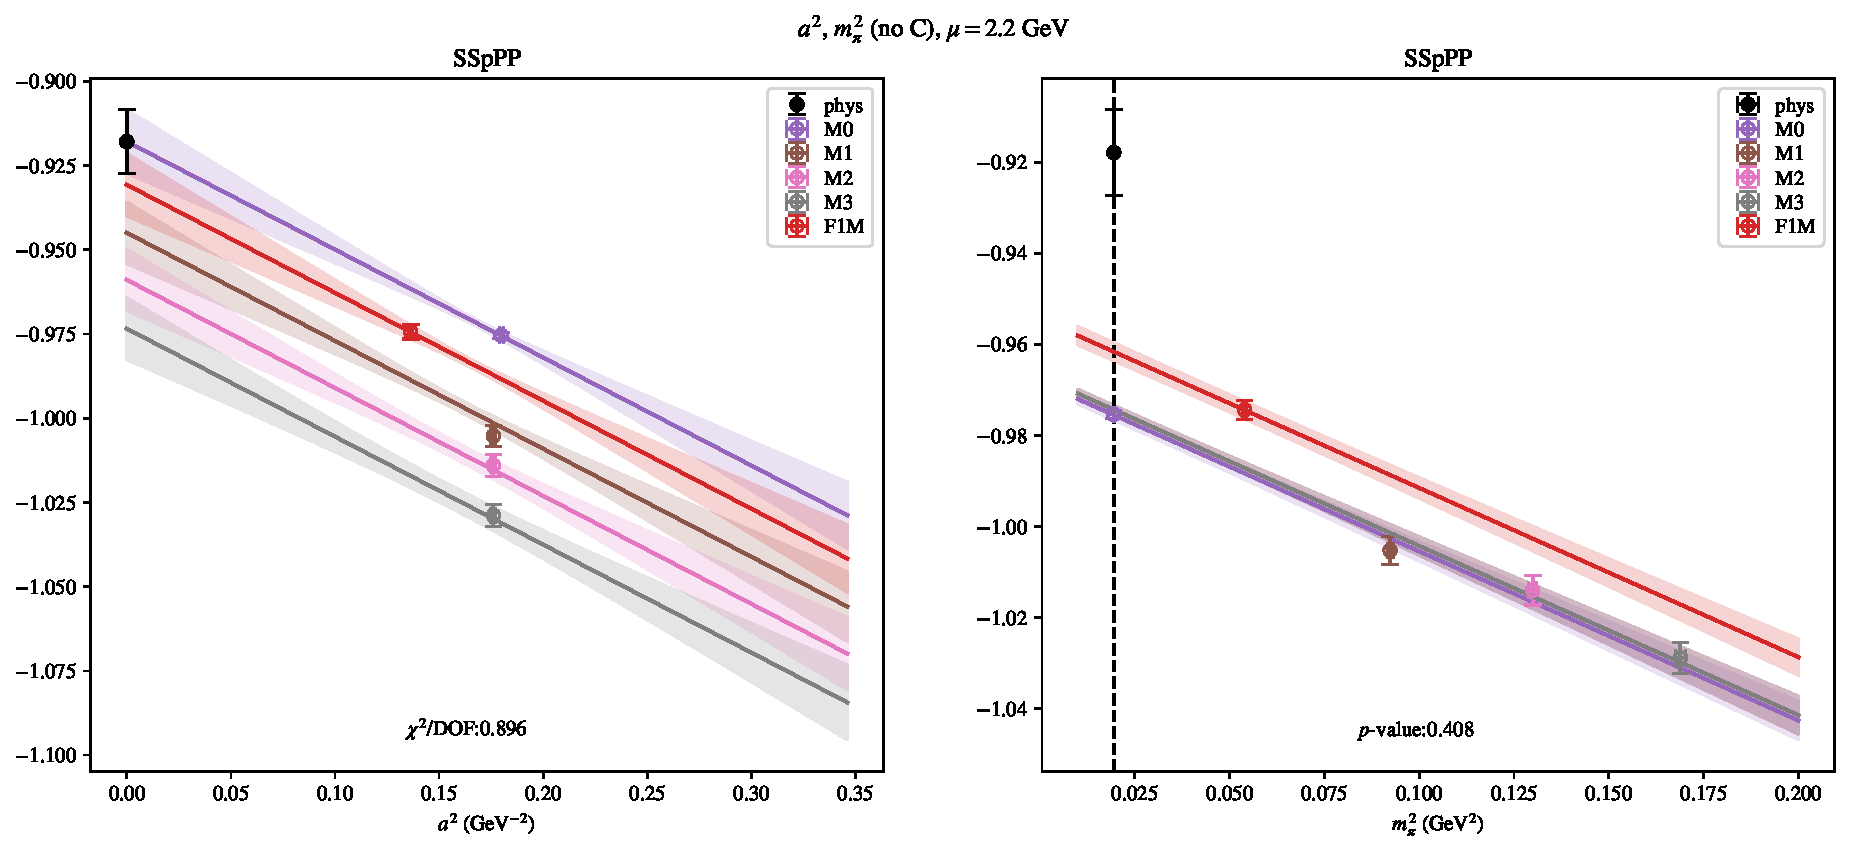
\includepdf[link, pages=-]{VVmAA/SUSY/bag_a2m2noC_22.pdf}
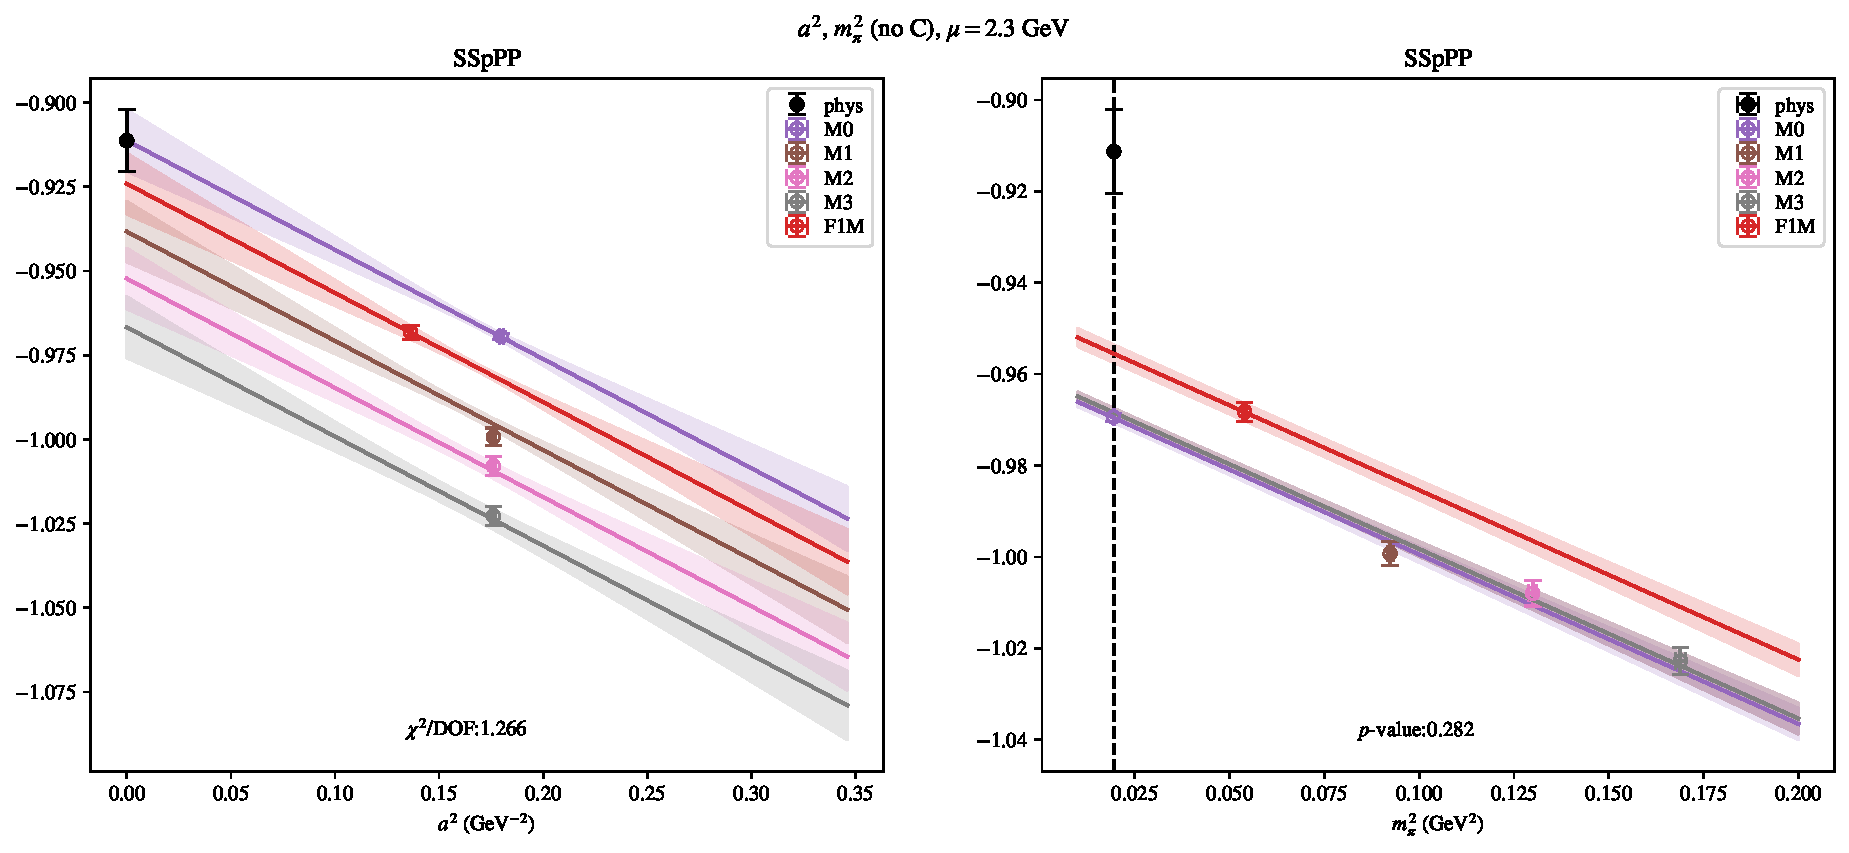
\includepdf[link, pages=-]{VVmAA/SUSY/bag_a2m2noC_23.pdf}
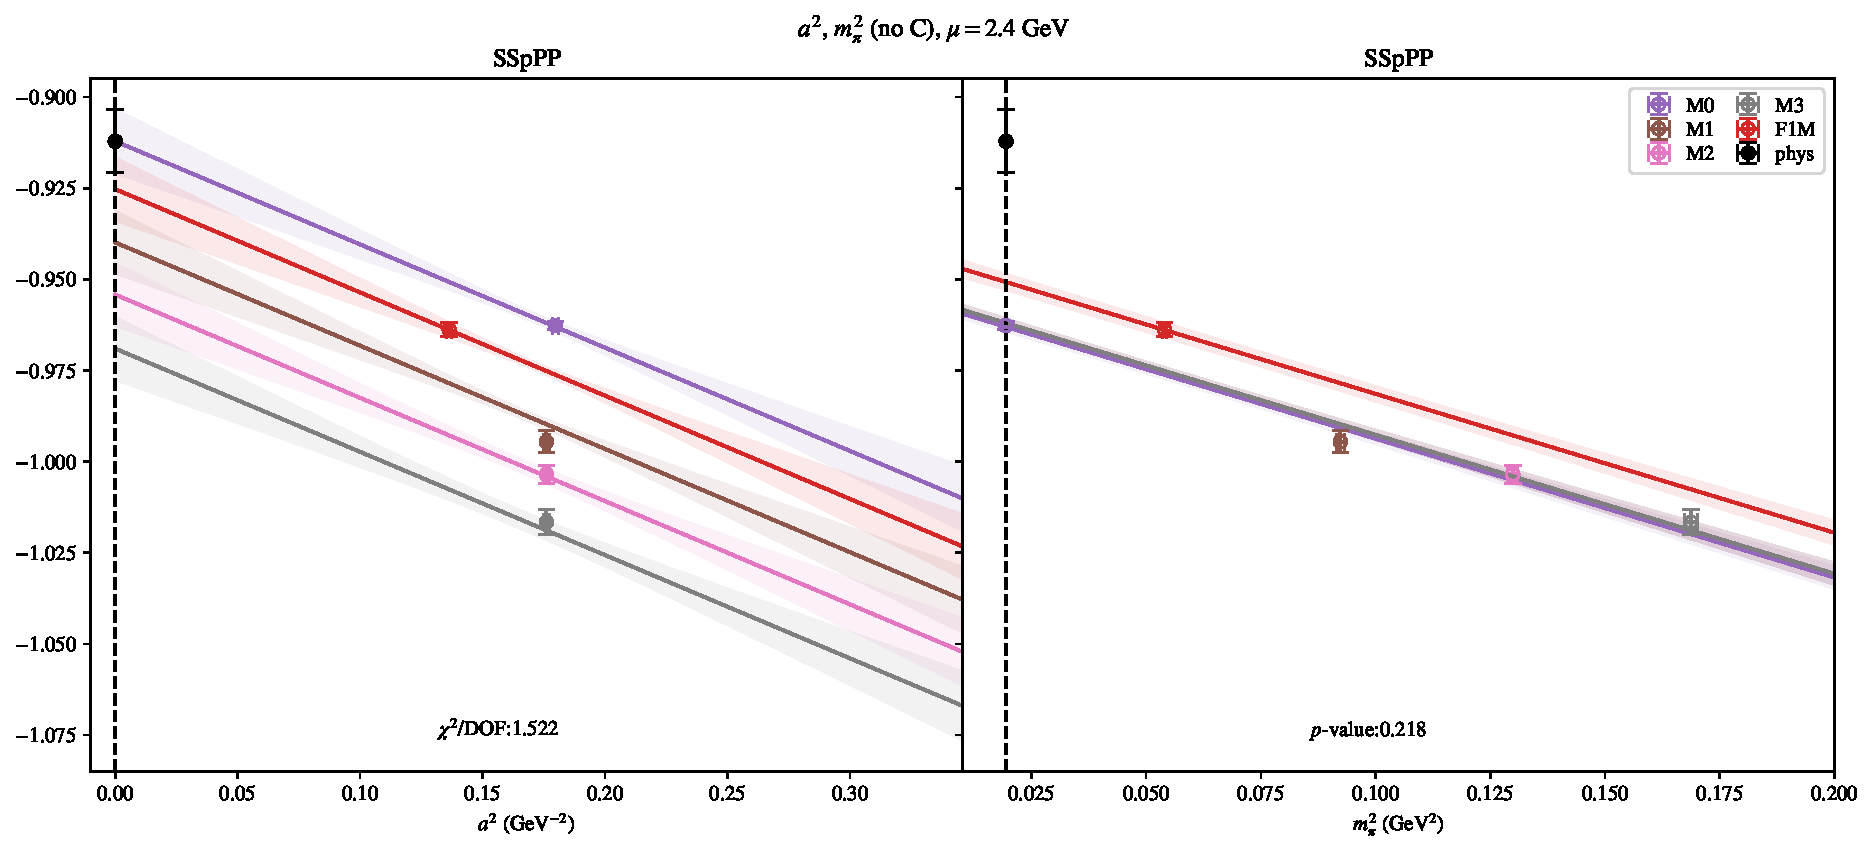
\includepdf[link, pages=-]{VVmAA/SUSY/bag_a2m2noC_24.pdf}
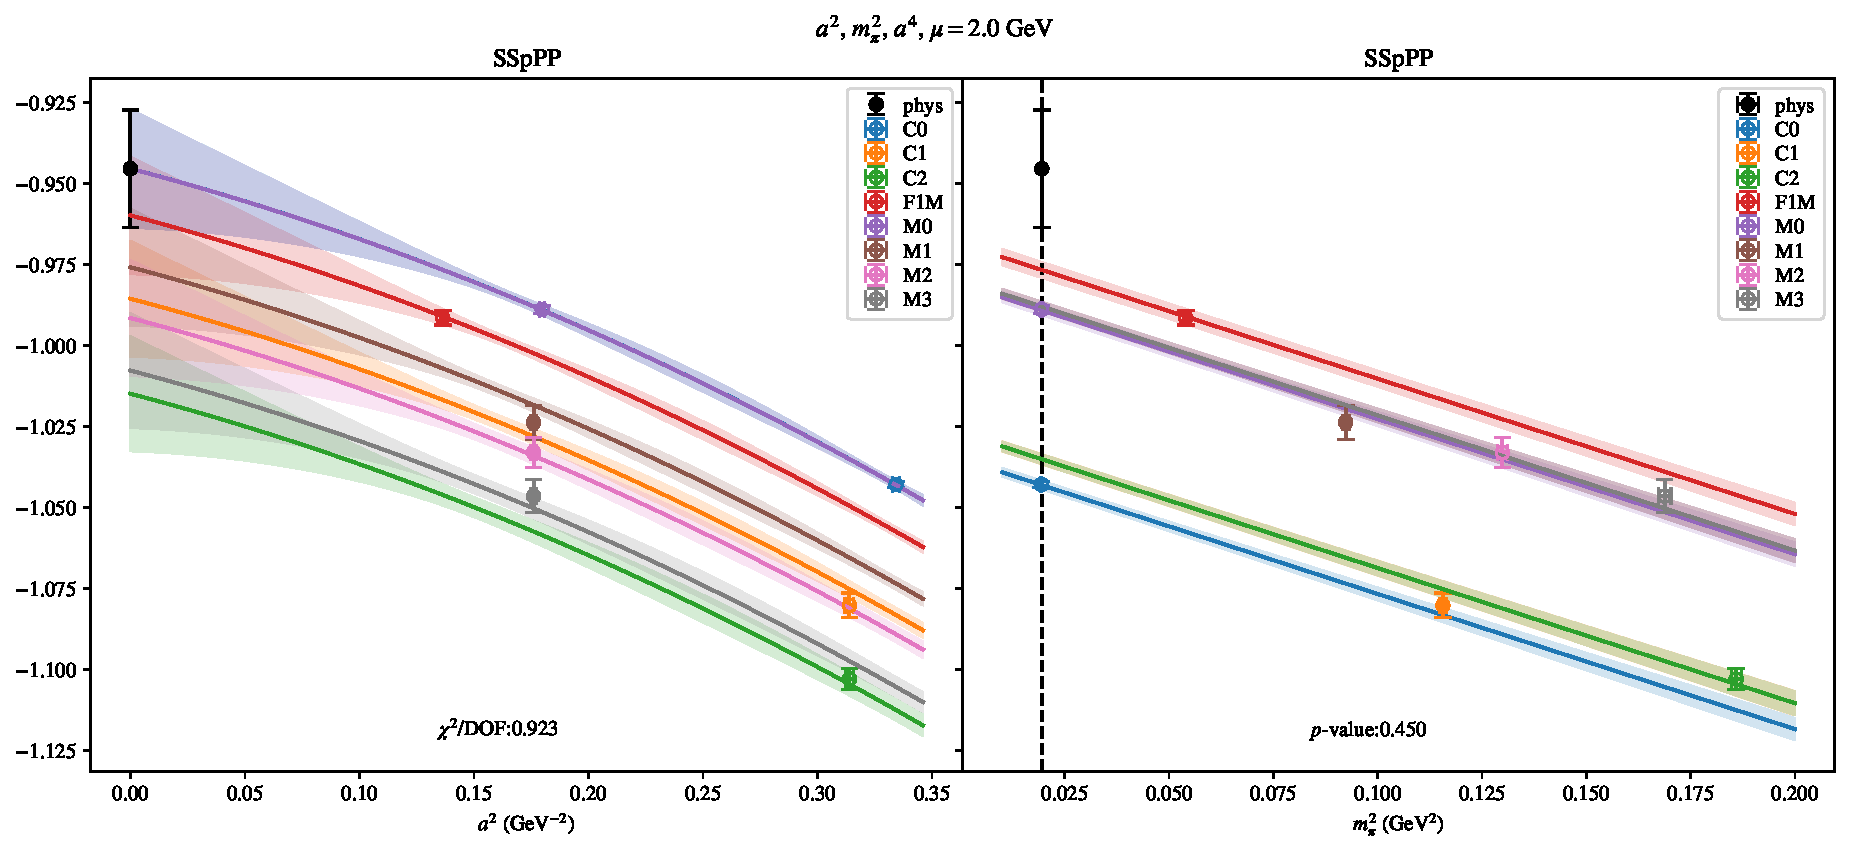
\includepdf[link, pages=-]{VVmAA/SUSY/bag_a2a4m2_20.pdf}
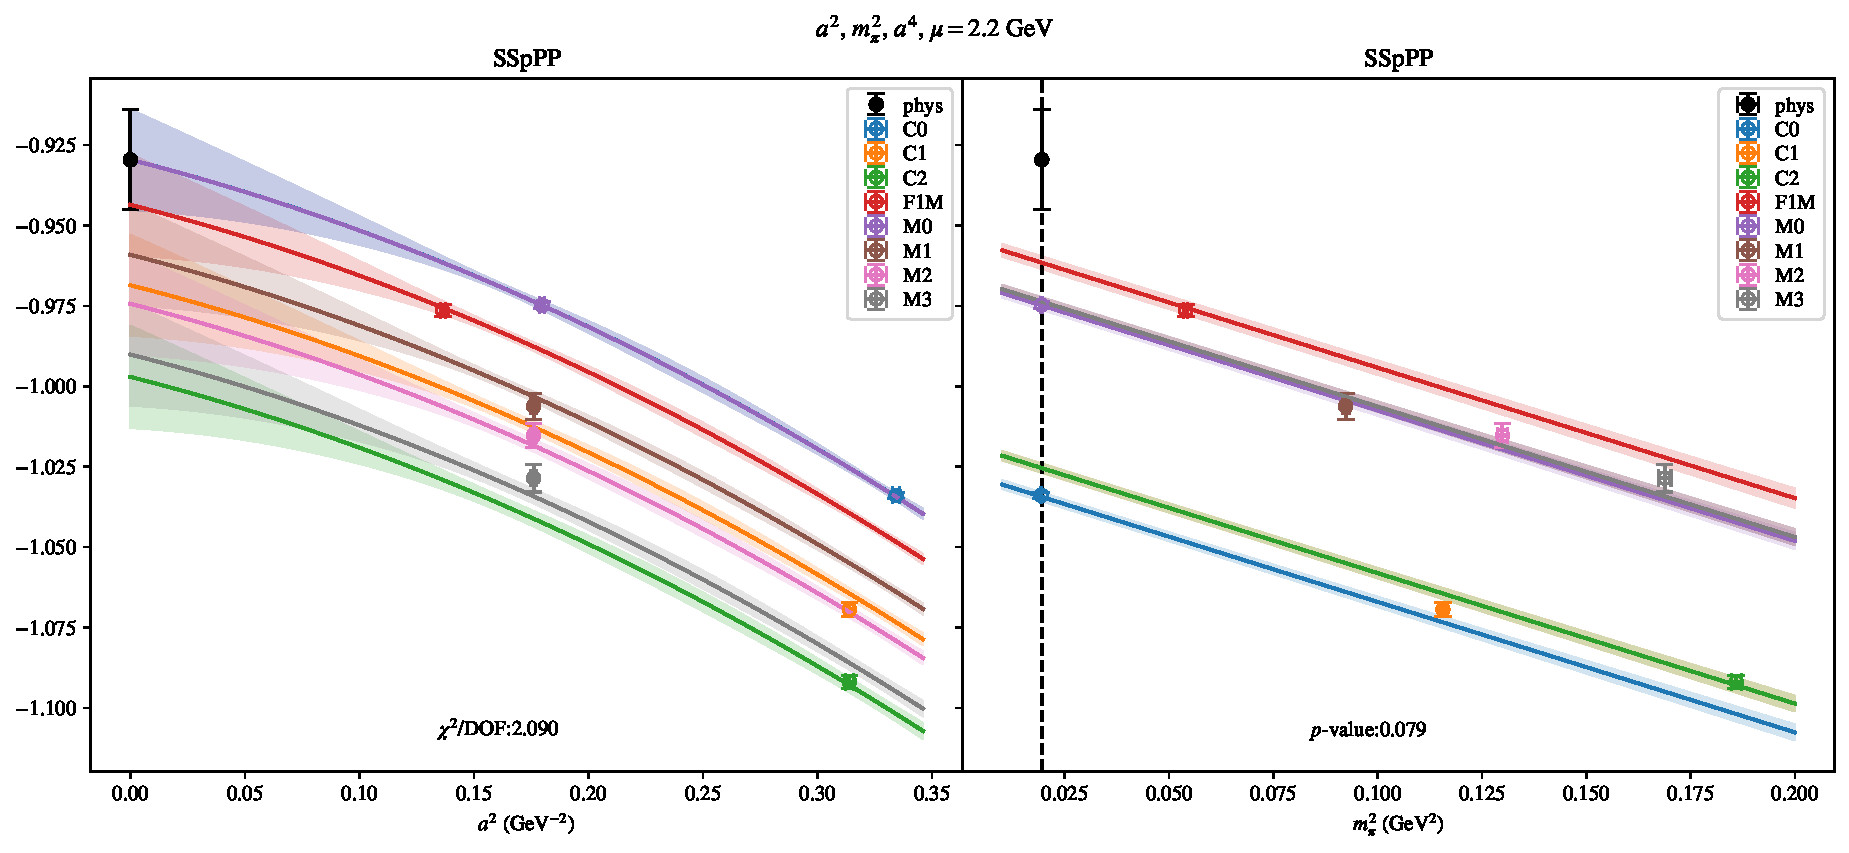
\includepdf[link, pages=-]{VVmAA/SUSY/bag_a2a4m2_22.pdf}
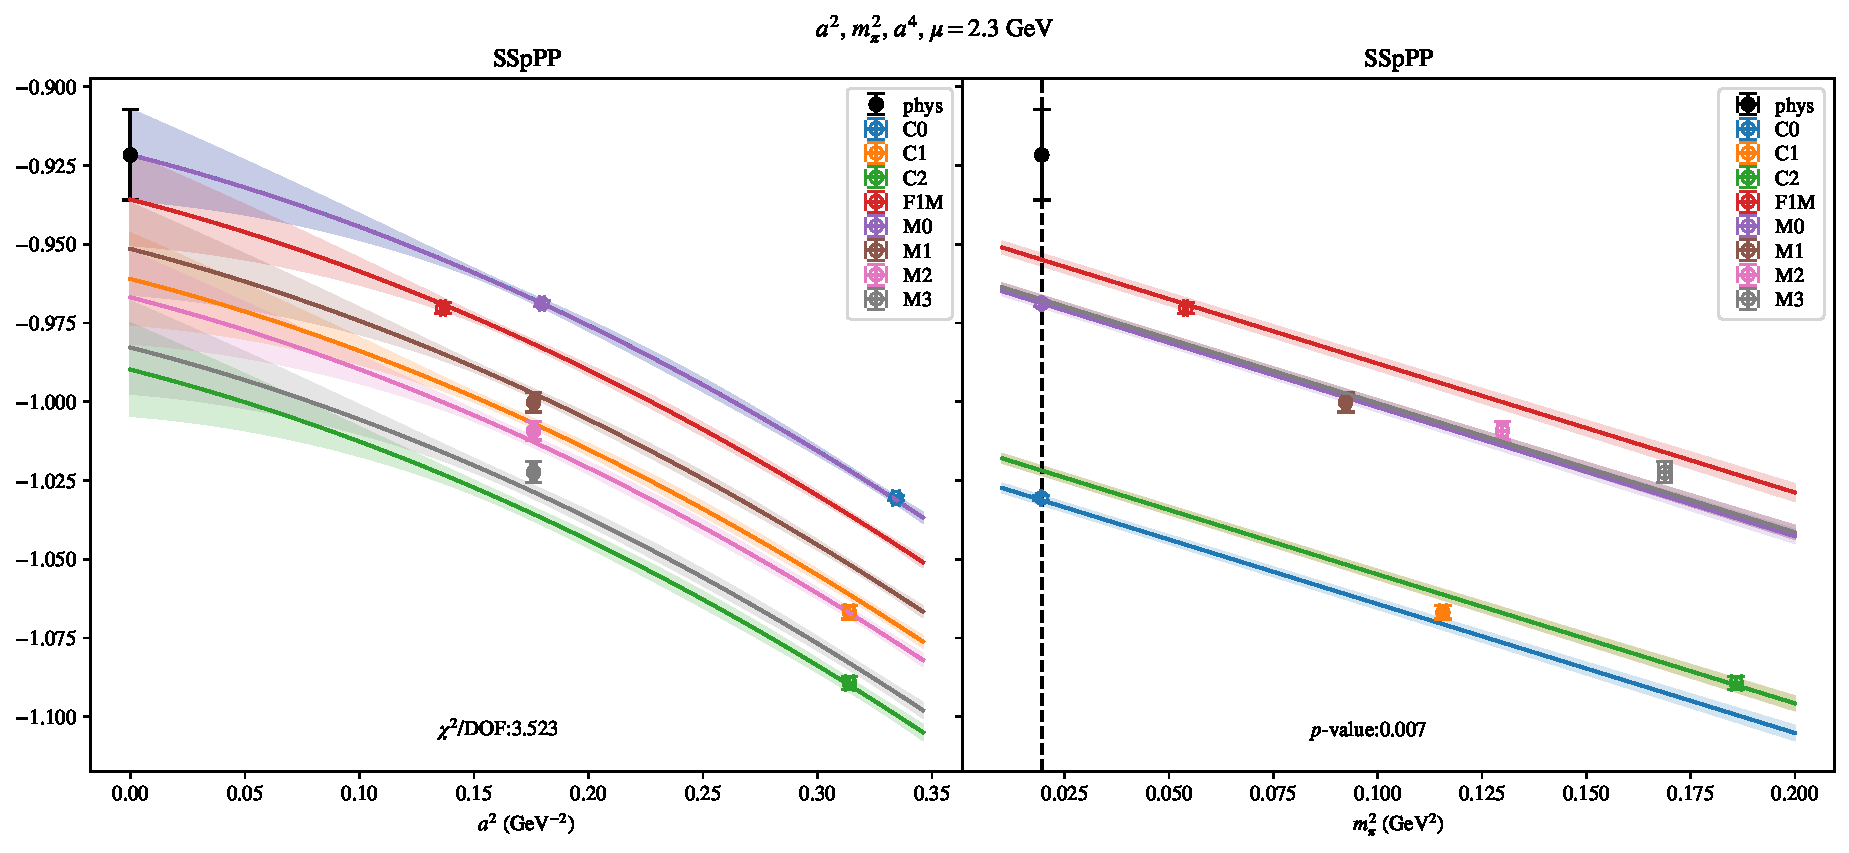
\includepdf[link, pages=-]{VVmAA/SUSY/bag_a2a4m2_23.pdf}
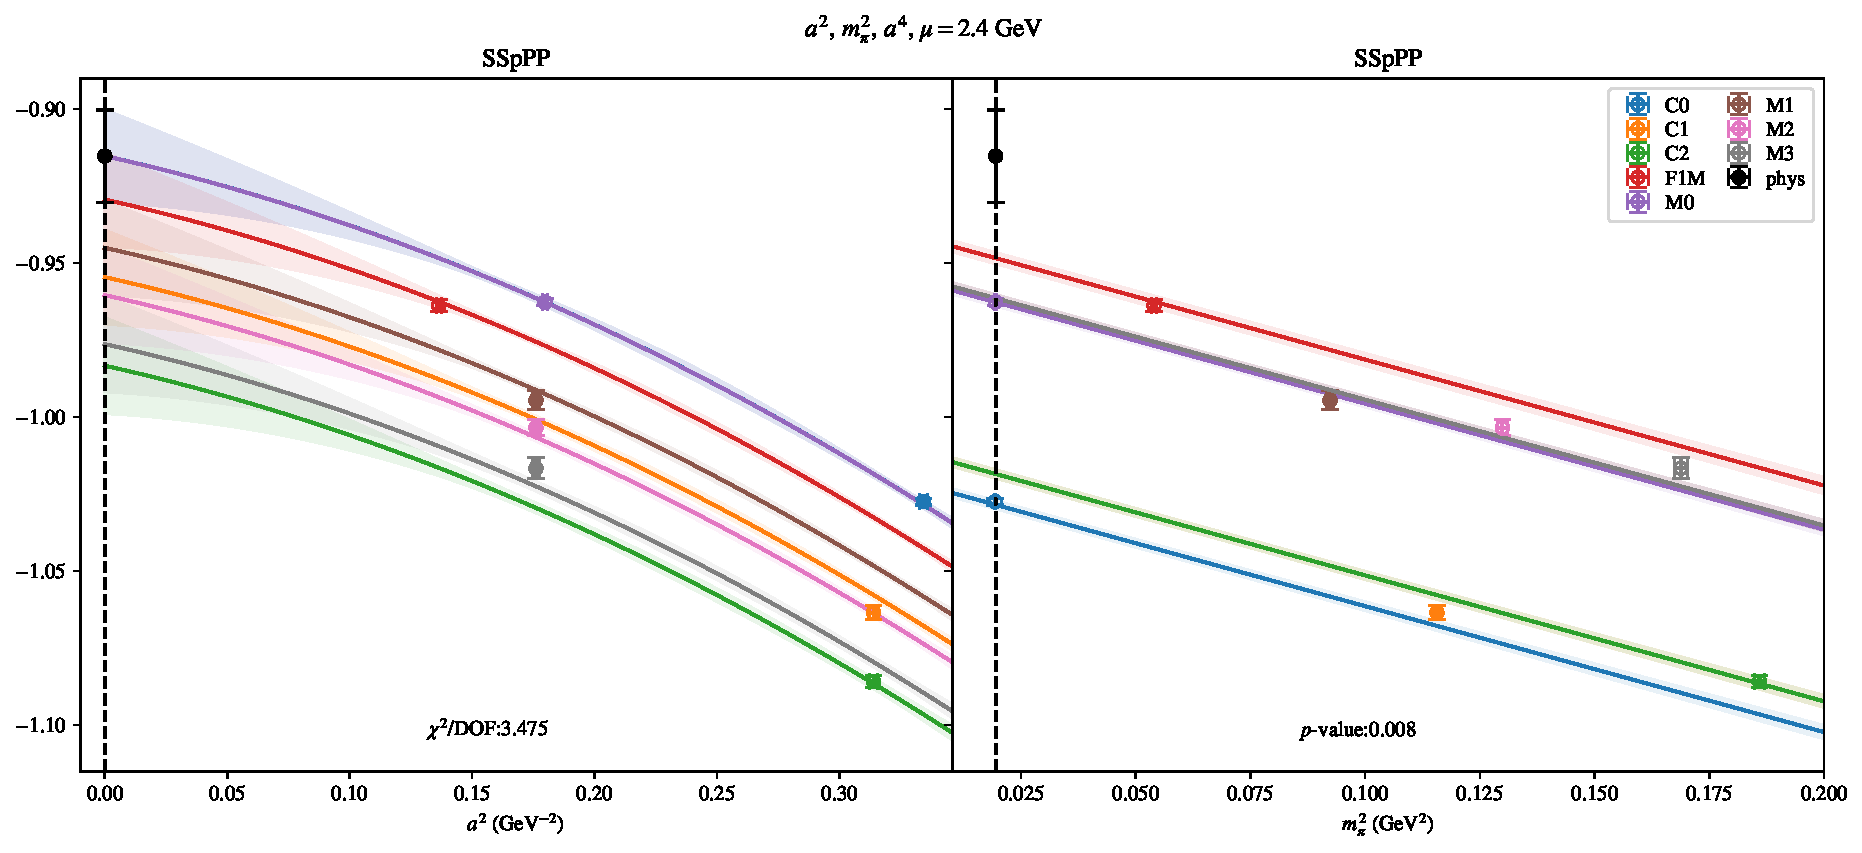
\includepdf[link, pages=-]{VVmAA/SUSY/bag_a2a4m2_24.pdf}
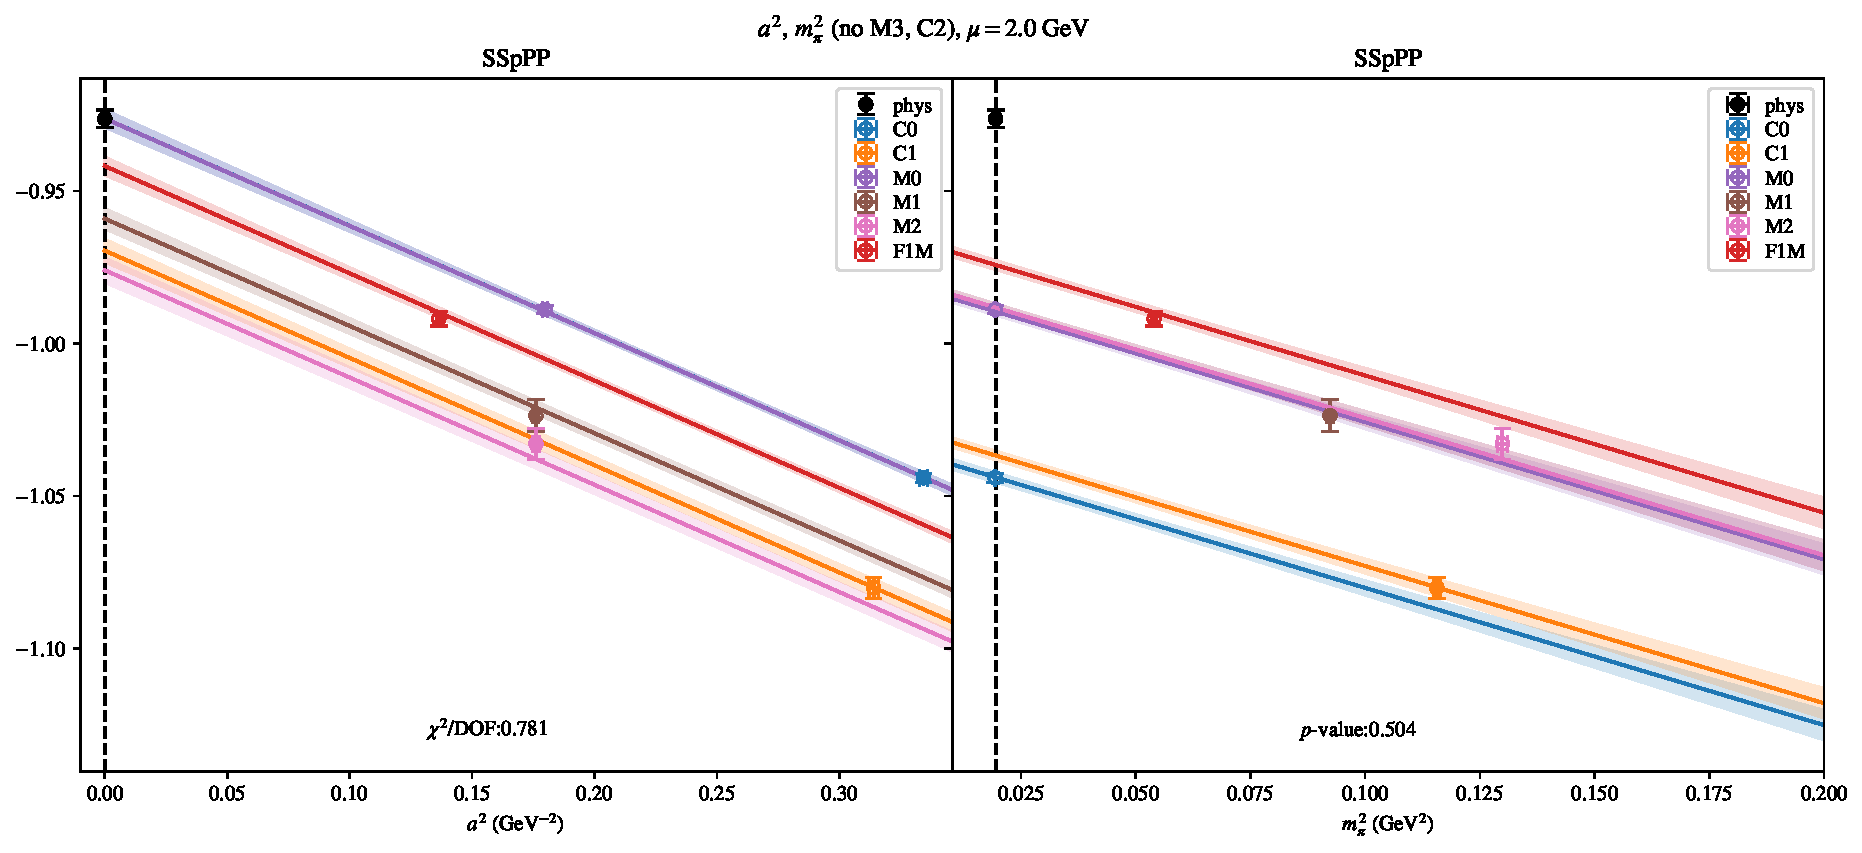
\includepdf[link, pages=-]{VVmAA/SUSY/bag_a2m2mcut_20.pdf}
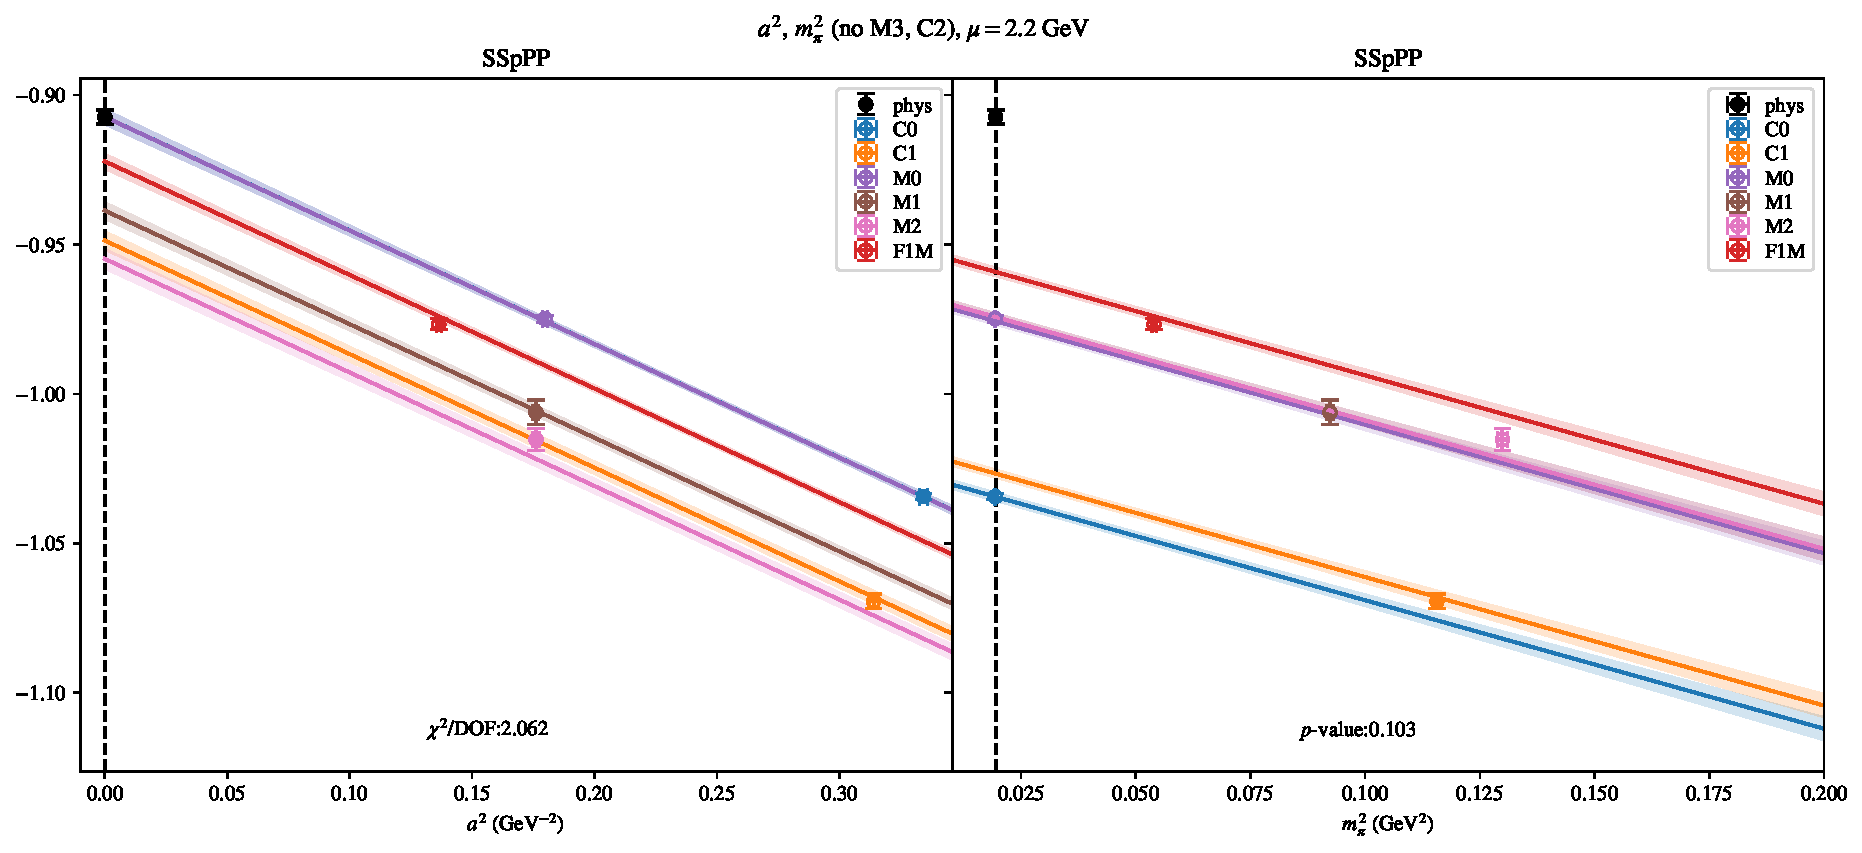
\includepdf[link, pages=-]{VVmAA/SUSY/bag_a2m2mcut_22.pdf}
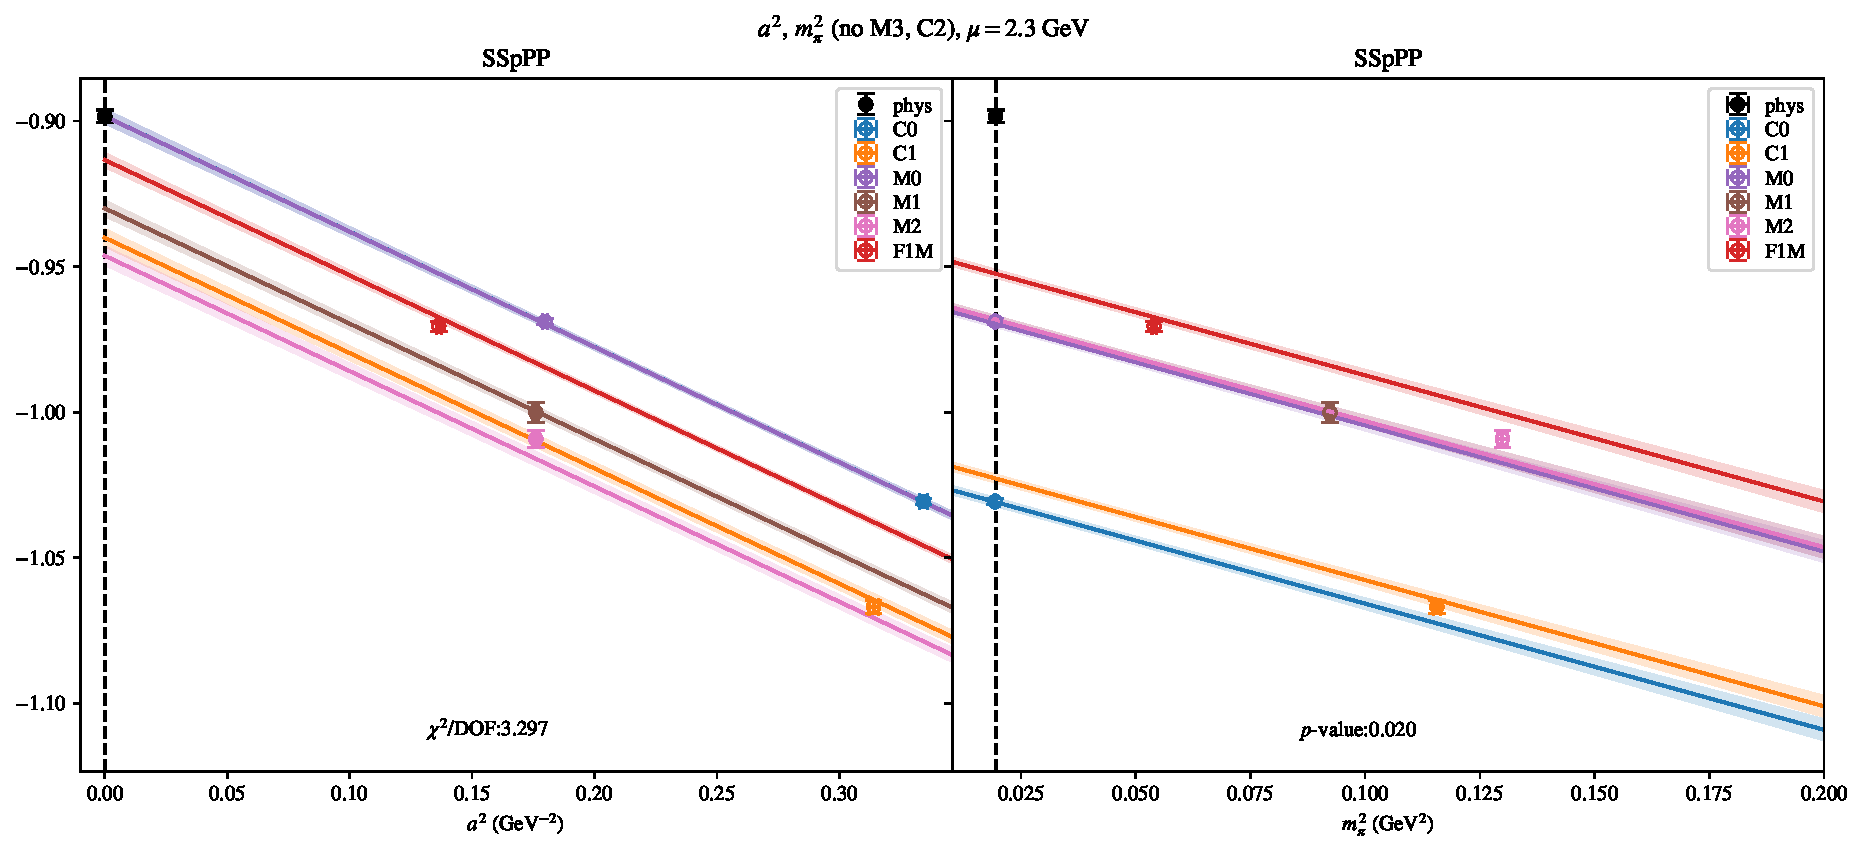
\includepdf[link, pages=-]{VVmAA/SUSY/bag_a2m2mcut_23.pdf}
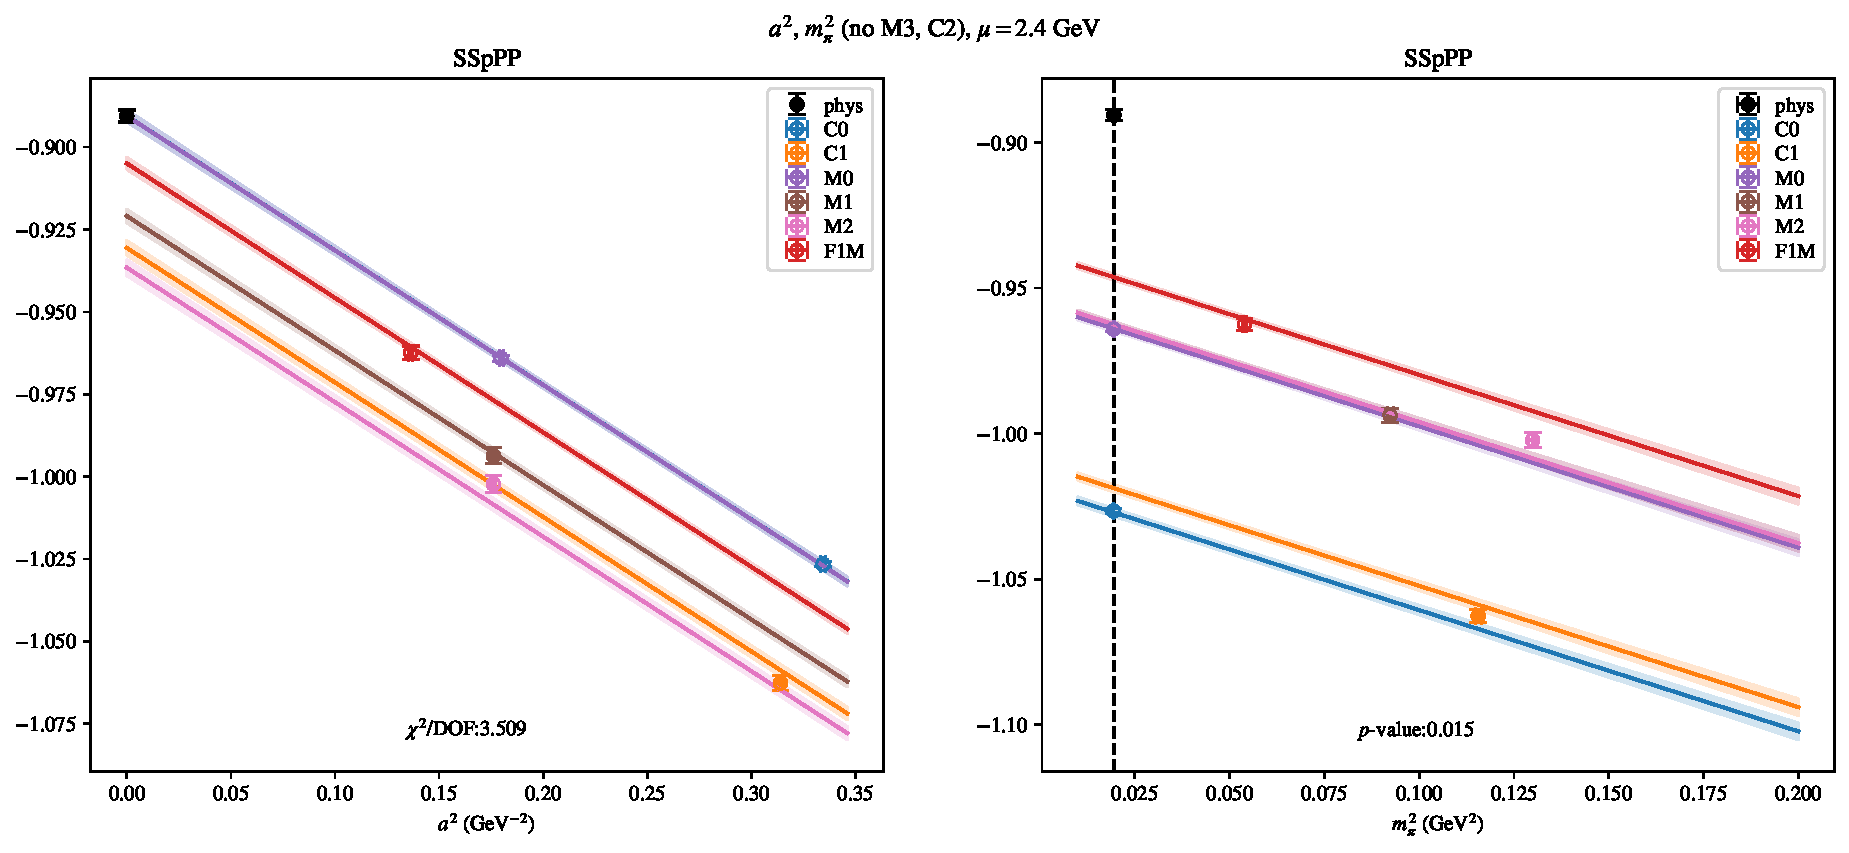
\includepdf[link, pages=-]{VVmAA/SUSY/bag_a2m2mcut_24.pdf}
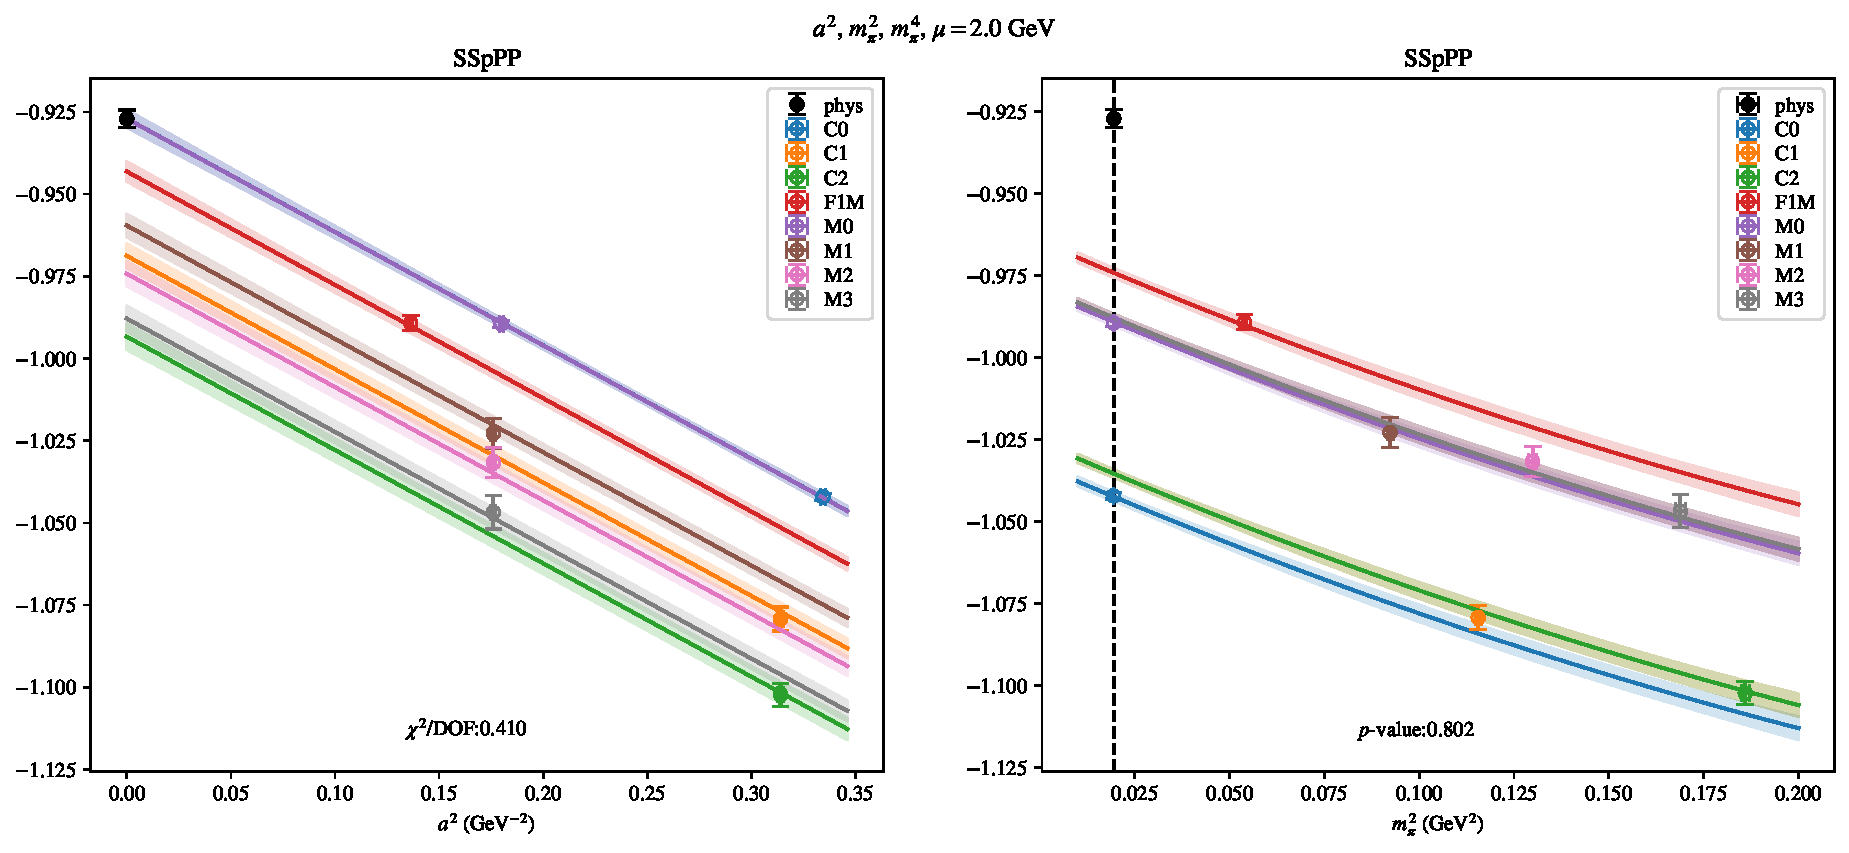
\includepdf[link, pages=-]{VVmAA/SUSY/bag_a2m2m4_20.pdf}
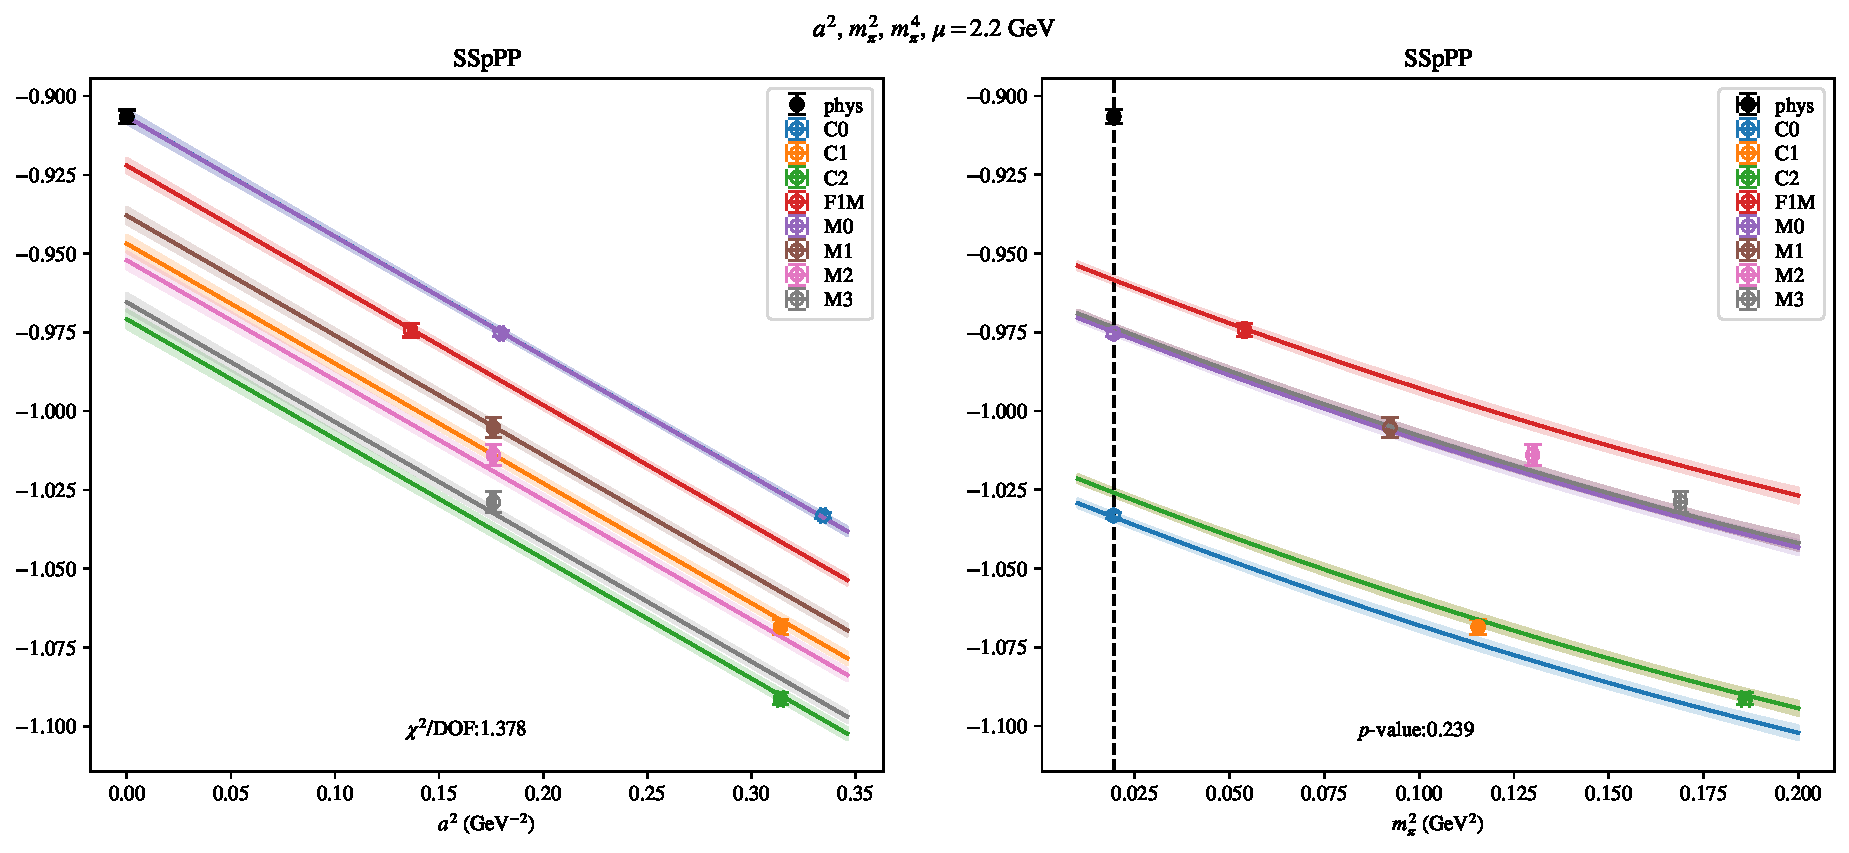
\includepdf[link, pages=-]{VVmAA/SUSY/bag_a2m2m4_22.pdf}
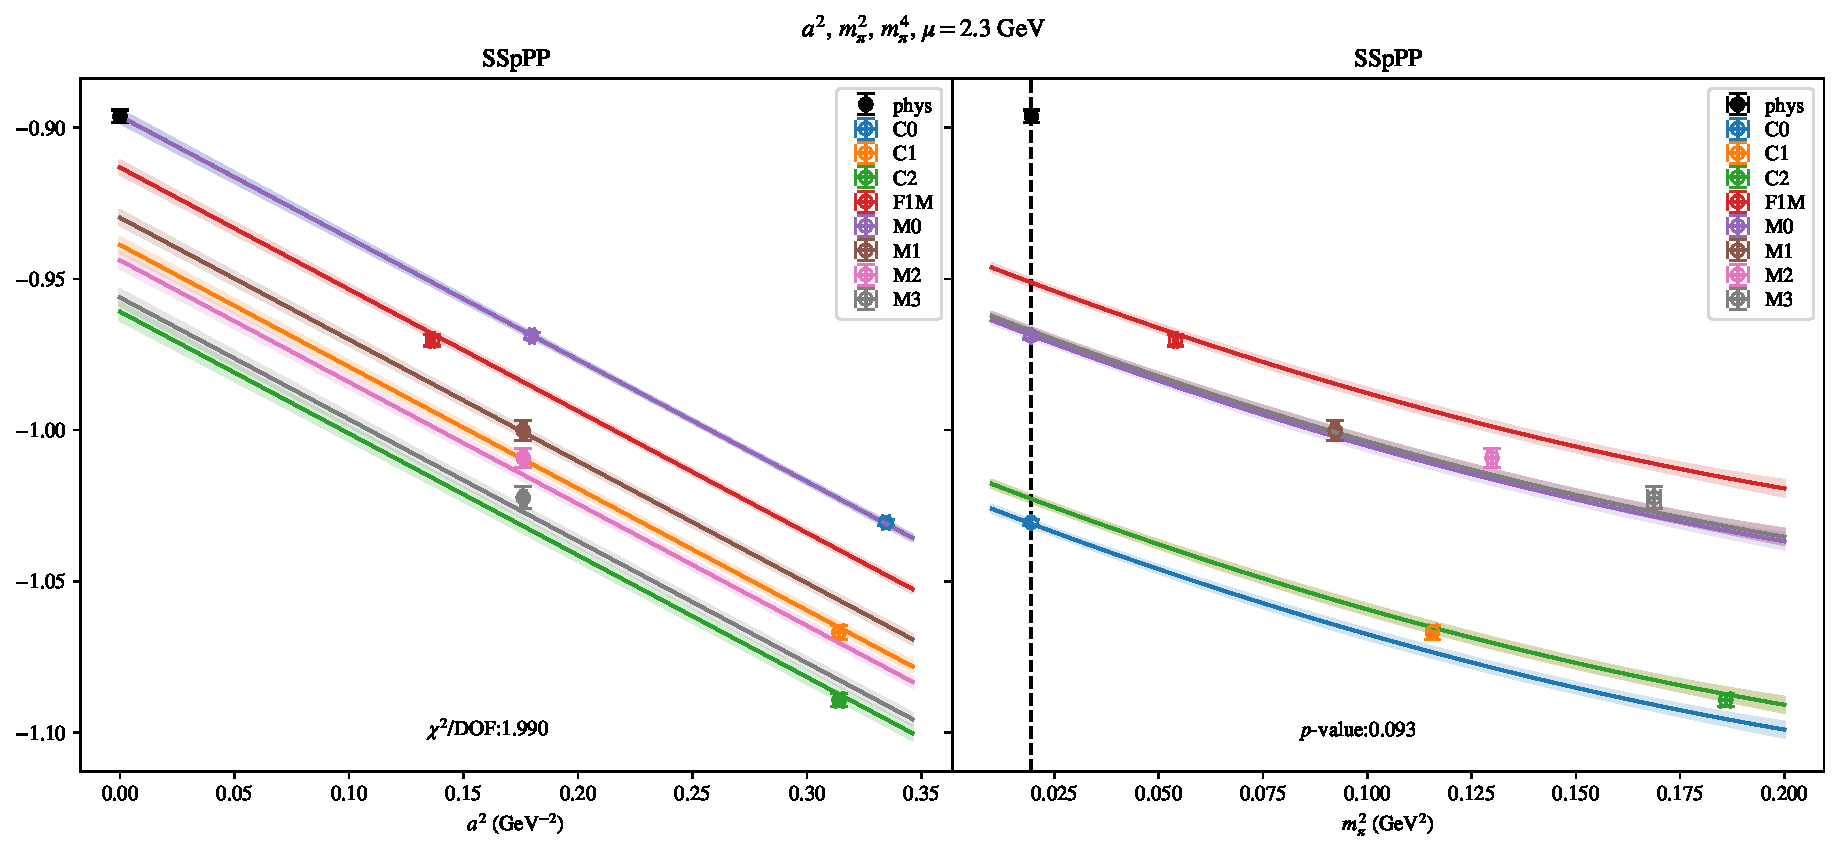
\includepdf[link, pages=-]{VVmAA/SUSY/bag_a2m2m4_23.pdf}
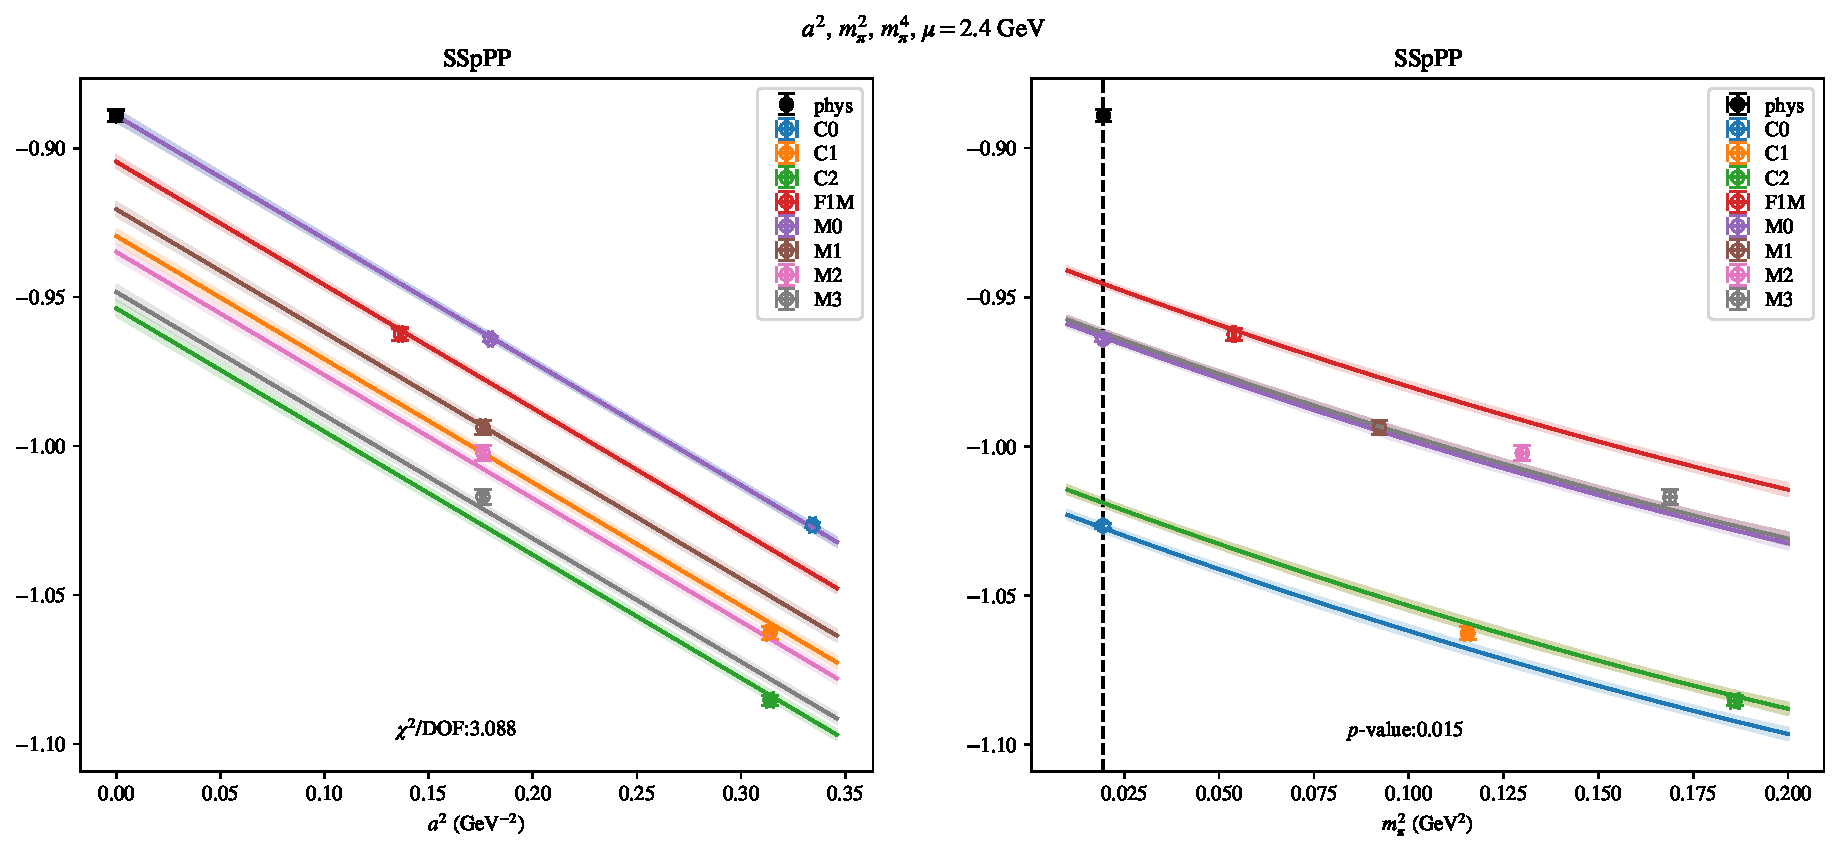
\includepdf[link, pages=-]{VVmAA/SUSY/bag_a2m2m4_24.pdf}
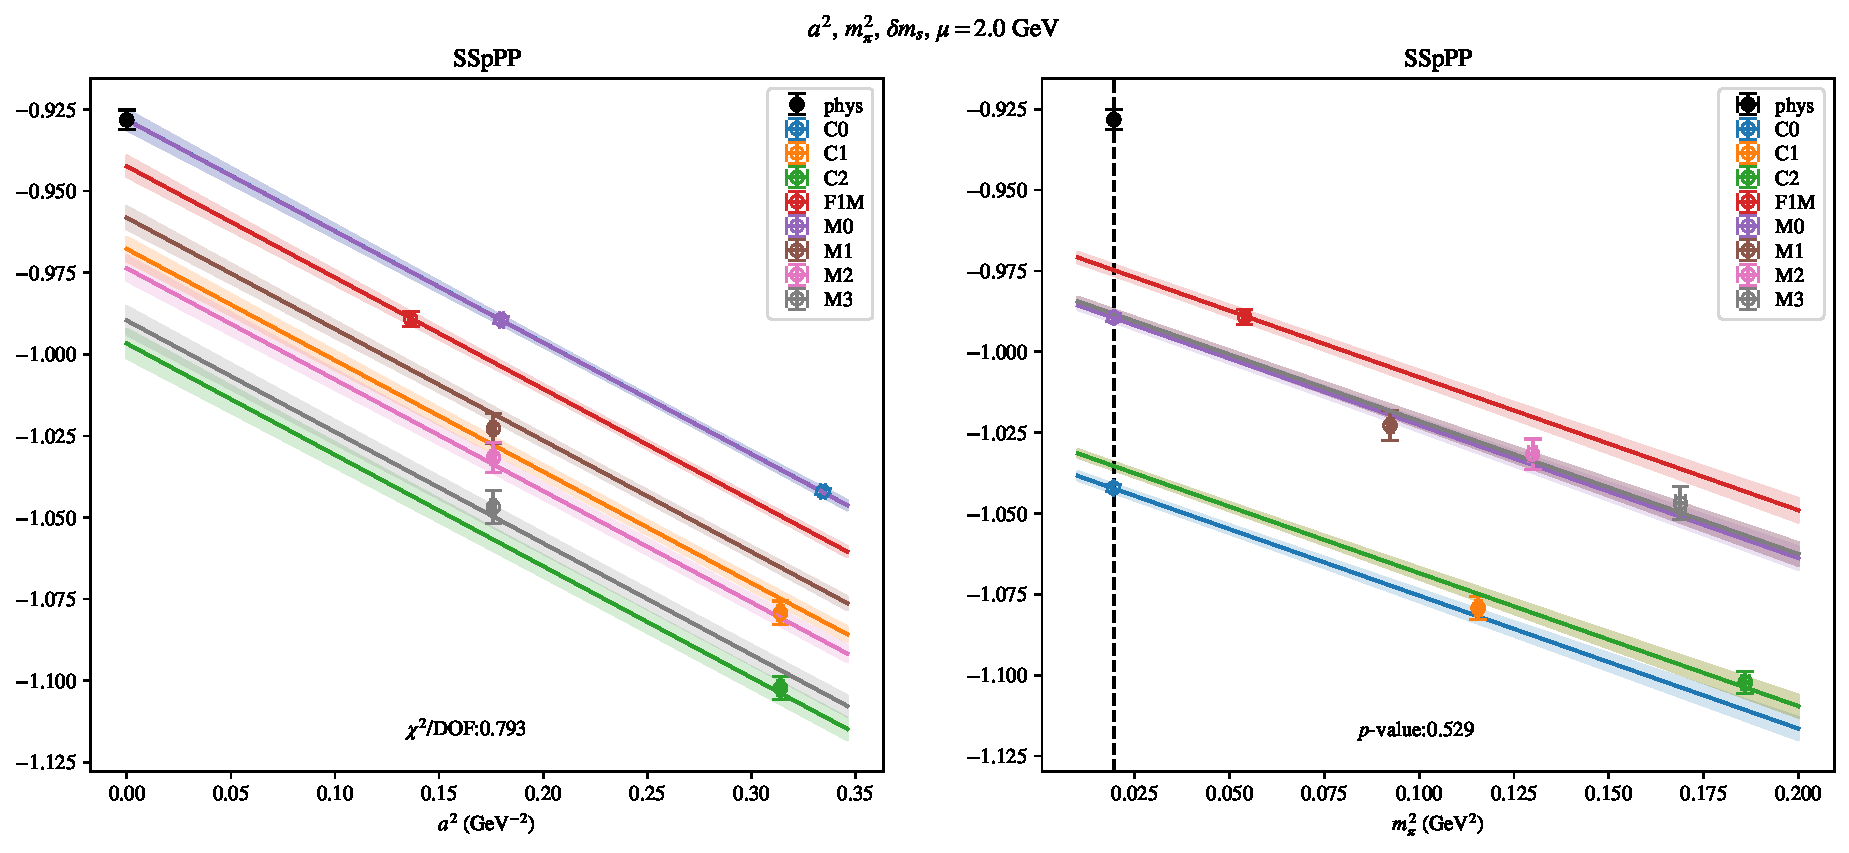
\includepdf[link, pages=-]{VVmAA/SUSY/bag_a2m2delm_20.pdf}
\includepdf[link, pages=-]{VVmAA/SUSY/bag_a2m2delm_22.pdf}
\includepdf[link, pages=-]{VVmAA/SUSY/bag_a2m2delm_23.pdf}
\includepdf[link, pages=-]{VVmAA/SUSY/bag_a2m2delm_24.pdf}
\clearpage
\section{$\mathcal{B}_3$}
\begin{table}[h!]
\begin{center}
\begin{tabular}{|c|c|c|c|c|c|c|}
\hline
$\mu$ (GeV) & $a^2$, $m_\pi^2$& $a^2$, $m_\pi^2$ (no C)& $a^2$, $m_\pi^2$, $a^4$& $a^2$, $m_\pi^2$ (no M3, C2)& $a^2$, $m_\pi^2$, $m_\pi^4$& $a^2$, $m_\pi^2$, $\delta m_s$\\
\hline
2.0& \hyperlink{SSmPP/SUSY/bag_a2m2_20.pdf.1}{\textbf{0.2827(46)}: 0.078 (0.996)} & \hyperlink{SSmPP/SUSY/bag_a2m2noC_20.pdf.1}{\textbf{0.286(21)}: 0.098 (0.907)} & \hyperlink{SSmPP/SUSY/bag_a2a4m2_20.pdf.1}{\textbf{0.286(36)}: 0.105 (0.981)} & \hyperlink{SSmPP/SUSY/bag_a2m2mcut_20.pdf.1}{\textbf{0.2822(41)}: 0.044 (0.988)} & \hyperlink{SSmPP/SUSY/bag_a2m2m4_20.pdf.1}{\textbf{0.2819(44)}: 0.016 (0.999)} & \hyperlink{SSmPP/SUSY/bag_a2m2delm_20.pdf.1}{\textbf{0.2822(50)}: 0.077 (0.989)}\\
2.2& \hyperlink{SSmPP/SUSY/bag_a2m2_22.pdf.1}{\textbf{0.2737(37)}: 0.101 (0.992)} & \hyperlink{SSmPP/SUSY/bag_a2m2noC_22.pdf.1}{\textbf{0.280(19)}: 0.102 (0.903)} & \hyperlink{SSmPP/SUSY/bag_a2a4m2_22.pdf.1}{\textbf{0.279(29)}: 0.143 (0.966)} & \hyperlink{SSmPP/SUSY/bag_a2m2mcut_22.pdf.1}{\textbf{0.2736(32)}: 0.082 (0.97)} & \hyperlink{SSmPP/SUSY/bag_a2m2m4_22.pdf.1}{\textbf{0.2731(40)}: 0.045 (0.996)} & \hyperlink{SSmPP/SUSY/bag_a2m2delm_22.pdf.1}{\textbf{0.2735(36)}: 0.139 (0.968)}\\
2.3& \hyperlink{SSmPP/SUSY/bag_a2m2_23.pdf.1}{\textbf{0.2698(36)}: 0.169 (0.974)} & \hyperlink{SSmPP/SUSY/bag_a2m2noC_23.pdf.1}{\textbf{0.277(19)}: 0.101 (0.904)} & \hyperlink{SSmPP/SUSY/bag_a2a4m2_23.pdf.1}{\textbf{0.274(27)}: 0.179 (0.949)} & \hyperlink{SSmPP/SUSY/bag_a2m2mcut_23.pdf.1}{\textbf{0.2697(33)}: 0.116 (0.951)} & \hyperlink{SSmPP/SUSY/bag_a2m2m4_23.pdf.1}{\textbf{0.2692(35)}: 0.084 (0.987)} & \hyperlink{SSmPP/SUSY/bag_a2m2delm_23.pdf.1}{\textbf{0.2694(32)}: 0.18 (0.949)}\\
2.4& \hyperlink{SSmPP/SUSY/bag_a2m2_24.pdf.1}{\textbf{0.2665(32)}: 0.232 (0.949)} & \hyperlink{SSmPP/SUSY/bag_a2m2noC_24.pdf.1}{\textbf{0.274(15)}: 0.118 (0.888)} & \hyperlink{SSmPP/SUSY/bag_a2a4m2_24.pdf.1}{\textbf{0.272(21)}: 0.257 (0.905)} & \hyperlink{SSmPP/SUSY/bag_a2m2mcut_24.pdf.1}{\textbf{0.2662(28)}: 0.171 (0.916)} & \hyperlink{SSmPP/SUSY/bag_a2m2m4_24.pdf.1}{\textbf{0.2657(33)}: 0.145 (0.965)} & \hyperlink{SSmPP/SUSY/bag_a2m2delm_24.pdf.1}{\textbf{0.2664(34)}: 0.256 (0.906)}\\
\hline
\end{tabular}
\caption{Physical point value from chiral and continuum extrapolation at renormalisation scale $\mu$. Entries are \textbf{value(error)}: $\chi^2/\text{DOF}$ ($p$-value).}
\end{center}
\end{table}
\begin{table}[h!]
\begin{center}
\begin{tabular}{|c c|c|c|c|c|c|c|}
\hline
$\mu$ (GeV) &  & $a^2$, $m_\pi^2$& $a^2$, $m_\pi^2$ (no C)& $a^2$, $m_\pi^2$, $a^4$& $a^2$, $m_\pi^2$ (no M3, C2)& $a^2$, $m_\pi^2$, $m_\pi^4$& $a^2$, $m_\pi^2$, $\delta m_s$\\
\hline
\multirow{3}{0.5in}{2.0} & $\alpha$ & 0.178(15)& 0.16(12)& 0.15(32)& 0.180(14)& 0.181(15)& 0.179(17)\\
 & $\beta$ & 0.00228(43)& 0.00229(80)& 0.00228(44)& 0.00252(58)& 0.0033(13)& 0.00209(71)\\
 & $\gamma$ &  &  & 0.06(64)&  & -0.000099(95)& 0.007(28)\\
\hline
\multirow{3}{0.5in}{2.2} & $\alpha$ & 0.204(13)& 0.17(11)& 0.16(26)& 0.204(11)& 0.206(14)& 0.204(12)\\
 & $\beta$ & 0.00221(37)& 0.00211(62)& 0.00221(35)& 0.00240(54)& 0.00315(98)& 0.00207(52)\\
 & $\gamma$ &  &  & 0.09(52)&  & -0.000087(71)& 0.005(22)\\
\hline
\multirow{3}{0.5in}{2.3} & $\alpha$ & 0.216(12)& 0.17(11)& 0.18(24)& 0.217(11)& 0.218(12)& 0.217(11)\\
 & $\beta$ & 0.00222(32)& 0.00209(61)& 0.00224(31)& 0.00242(49)& 0.0031(10)& 0.00207(55)\\
 & $\gamma$ &  &  & 0.08(48)&  & -0.000087(76)& 0.006(21)\\
\hline
\multirow{3}{0.5in}{2.4} & $\alpha$ & 0.227(11)& 0.183(89)& 0.18(18)& 0.228(10)& 0.229(11)& 0.227(12)\\
 & $\beta$ & 0.00221(30)& 0.00205(54)& 0.00224(28)& 0.00242(39)& 0.00315(76)& 0.00215(44)\\
 & $\gamma$ &  &  & 0.10(38)&  & -0.000086(56)& 0.003(19)\\
\hline
\end{tabular}
\caption{Fit values of coefficients in $Q = Q_{phys} + \mathbf{\alpha} a^2 + \mathbf{\beta}\left(\frac{m_\pi^2}{f_\pi^2}-\frac{m_{\pi,PDG}^2}{f_\pi^2}\right) + \gamma(\ldots)$}
\end{center}
\end{table}
\includepdf[link, pages=-]{SSmPP/SUSY/bag_a2m2_20.pdf}
\includepdf[link, pages=-]{SSmPP/SUSY/bag_a2m2_22.pdf}
\includepdf[link, pages=-]{SSmPP/SUSY/bag_a2m2_23.pdf}
\includepdf[link, pages=-]{SSmPP/SUSY/bag_a2m2_24.pdf}
\includepdf[link, pages=-]{SSmPP/SUSY/bag_a2m2noC_20.pdf}
\includepdf[link, pages=-]{SSmPP/SUSY/bag_a2m2noC_22.pdf}
\includepdf[link, pages=-]{SSmPP/SUSY/bag_a2m2noC_23.pdf}
\includepdf[link, pages=-]{SSmPP/SUSY/bag_a2m2noC_24.pdf}
\includepdf[link, pages=-]{SSmPP/SUSY/bag_a2a4m2_20.pdf}
\includepdf[link, pages=-]{SSmPP/SUSY/bag_a2a4m2_22.pdf}
\includepdf[link, pages=-]{SSmPP/SUSY/bag_a2a4m2_23.pdf}
\includepdf[link, pages=-]{SSmPP/SUSY/bag_a2a4m2_24.pdf}
\includepdf[link, pages=-]{SSmPP/SUSY/bag_a2m2mcut_20.pdf}
\includepdf[link, pages=-]{SSmPP/SUSY/bag_a2m2mcut_22.pdf}
\includepdf[link, pages=-]{SSmPP/SUSY/bag_a2m2mcut_23.pdf}
\includepdf[link, pages=-]{SSmPP/SUSY/bag_a2m2mcut_24.pdf}
\includepdf[link, pages=-]{SSmPP/SUSY/bag_a2m2m4_20.pdf}
\includepdf[link, pages=-]{SSmPP/SUSY/bag_a2m2m4_22.pdf}
\includepdf[link, pages=-]{SSmPP/SUSY/bag_a2m2m4_23.pdf}
\includepdf[link, pages=-]{SSmPP/SUSY/bag_a2m2m4_24.pdf}
\includepdf[link, pages=-]{SSmPP/SUSY/bag_a2m2delm_20.pdf}
\includepdf[link, pages=-]{SSmPP/SUSY/bag_a2m2delm_22.pdf}
\includepdf[link, pages=-]{SSmPP/SUSY/bag_a2m2delm_23.pdf}
\includepdf[link, pages=-]{SSmPP/SUSY/bag_a2m2delm_24.pdf}
\clearpage
\section{$\mathcal{B}_4$}
\begin{table}[h!]
\begin{center}
\begin{tabular}{|c|c|c|c|c|c|c|}
\hline
$\mu$ (GeV) & $a^2$, $m_\pi^2$& $a^2$, $m_\pi^2$ (no C)& $a^2$, $m_\pi^2$, $a^4$& $a^2$, $m_\pi^2$ (no M3, C2)& $a^2$, $m_\pi^2$, $m_\pi^4$& $a^2$, $m_\pi^2$, $\delta m_s$\\
\hline
2.0& \hyperlink{SSpPP/SUSY/bag_a2m2_20.pdf.1}{\textbf{1.8011(51)}: 5.852 (0.0)} & \hyperlink{SSpPP/SUSY/bag_a2m2noC_20.pdf.1}{\textbf{1.696(19)}: 0.047 (0.954)} & \hyperlink{SSpPP/SUSY/bag_a2a4m2_20.pdf.1}{\textbf{1.635(31)}: 0.747 (0.56)} & \hyperlink{SSpPP/SUSY/bag_a2m2mcut_20.pdf.1}{\textbf{1.7993(41)}: 12.792 (0.0)} & \hyperlink{SSpPP/SUSY/bag_a2m2m4_20.pdf.1}{\textbf{1.8045(48)}: 6.346 (0.0)} & \hyperlink{SSpPP/SUSY/bag_a2m2delm_20.pdf.1}{\textbf{1.7973(59)}: 2.656 (0.031)}\\
2.2& \hyperlink{SSpPP/SUSY/bag_a2m2_22.pdf.1}{\textbf{1.8024(38)}: 7.554 (0.0)} & \hyperlink{SSpPP/SUSY/bag_a2m2noC_22.pdf.1}{\textbf{1.715(16)}: 0.157 (0.854)} & \hyperlink{SSpPP/SUSY/bag_a2a4m2_22.pdf.1}{\textbf{1.661(24)}: 0.915 (0.454)} & \hyperlink{SSpPP/SUSY/bag_a2m2mcut_22.pdf.1}{\textbf{1.8027(40)}: 12.17 (0.0)} & \hyperlink{SSpPP/SUSY/bag_a2m2m4_22.pdf.1}{\textbf{1.8077(44)}: 6.73 (0.0)} & \hyperlink{SSpPP/SUSY/bag_a2m2delm_22.pdf.1}{\textbf{1.8019(50)}: 4.322 (0.002)}\\
2.3& \hyperlink{SSpPP/SUSY/bag_a2m2_23.pdf.1}{\textbf{1.8037(35)}: 8.138 (0.0)} & \hyperlink{SSpPP/SUSY/bag_a2m2noC_23.pdf.1}{\textbf{1.721(14)}: 0.19 (0.827)} & \hyperlink{SSpPP/SUSY/bag_a2a4m2_23.pdf.1}{\textbf{1.666(23)}: 0.707 (0.587)} & \hyperlink{SSpPP/SUSY/bag_a2m2mcut_23.pdf.1}{\textbf{1.8057(35)}: 11.864 (0.0)} & \hyperlink{SSpPP/SUSY/bag_a2m2m4_23.pdf.1}{\textbf{1.8081(41)}: 7.679 (0.0)} & \hyperlink{SSpPP/SUSY/bag_a2m2delm_23.pdf.1}{\textbf{1.8037(42)}: 4.35 (0.002)}\\
2.4& \hyperlink{SSpPP/SUSY/bag_a2m2_24.pdf.1}{\textbf{1.8055(32)}: 8.226 (0.0)} & \hyperlink{SSpPP/SUSY/bag_a2m2noC_24.pdf.1}{\textbf{1.726(13)}: 0.244 (0.784)} & \hyperlink{SSpPP/SUSY/bag_a2a4m2_24.pdf.1}{\textbf{1.673(22)}: 0.786 (0.534)} & \hyperlink{SSpPP/SUSY/bag_a2m2mcut_24.pdf.1}{\textbf{1.8063(35)}: 12.586 (0.0)} & \hyperlink{SSpPP/SUSY/bag_a2m2m4_24.pdf.1}{\textbf{1.8089(37)}: 8.059 (0.0)} & \hyperlink{SSpPP/SUSY/bag_a2m2delm_24.pdf.1}{\textbf{1.8052(38)}: 4.421 (0.001)}\\
\hline
\end{tabular}
\caption{Physical point value from chiral and continuum extrapolation at renormalisation scale $\mu$. Entries are \textbf{value(error)}: $\chi^2/\text{DOF}$ ($p$-value).}
\end{center}
\end{table}
\begin{table}[h!]
\begin{center}
\begin{tabular}{|c c|c|c|c|c|c|c|}
\hline
$\mu$ (GeV) &  & $a^2$, $m_\pi^2$& $a^2$, $m_\pi^2$ (no C)& $a^2$, $m_\pi^2$, $a^4$& $a^2$, $m_\pi^2$ (no M3, C2)& $a^2$, $m_\pi^2$, $m_\pi^4$& $a^2$, $m_\pi^2$, $\delta m_s$\\
\hline
\multirow{3}{0.5in}{2.0} & $\alpha$ & 0.123(18)& 0.74(11)& 1.62(28)& 0.130(15)& 0.113(17)& 0.127(20)\\
 & $\beta$ & -0.00039(50)& 0.0001(10)& -0.00082(53)& -0.00133(72)& -0.0066(15)& -0.00393(80)\\
 & $\gamma$ &  &  & -3.00(58)&  & 0.00058(12)& 0.144(31)\\
\hline
\multirow{3}{0.5in}{2.2} & $\alpha$ & 0.144(13)& 0.665(99)& 1.44(22)& 0.143(14)& 0.128(15)& 0.138(18)\\
 & $\beta$ & -0.00070(37)& -0.00054(73)& -0.00121(33)& -0.00132(57)& -0.0059(13)& -0.00321(62)\\
 & $\gamma$ &  &  & -2.62(45)&  & 0.00047(11)& 0.102(24)\\
\hline
\multirow{3}{0.5in}{2.3} & $\alpha$ & 0.150(13)& 0.644(85)& 1.41(21)& 0.144(12)& 0.137(14)& 0.143(15)\\
 & $\beta$ & -0.00045(34)& -0.00050(65)& -0.00097(32)& -0.00096(51)& -0.0045(11)& -0.00296(61)\\
 & $\gamma$ &  &  & -2.55(43)&  & 0.00038(10)& 0.101(22)\\
\hline
\multirow{3}{0.5in}{2.4} & $\alpha$ & 0.152(11)& 0.629(79)& 1.36(21)& 0.150(12)& 0.142(13)& 0.147(13)\\
 & $\beta$ & -0.00033(26)& -0.00042(54)& -0.00089(25)& -0.00070(43)& -0.0039(12)& -0.00262(58)\\
 & $\gamma$ &  &  & -2.45(42)&  & 0.00033(10)& 0.090(21)\\
\hline
\end{tabular}
\caption{Fit values of coefficients in $Q = Q_{phys} + \mathbf{\alpha} a^2 + \mathbf{\beta}\left(\frac{m_\pi^2}{f_\pi^2}-\frac{m_{\pi,PDG}^2}{f_\pi^2}\right) + \gamma(\ldots)$}
\end{center}
\end{table}
\includepdf[link, pages=-]{SSpPP/SUSY/bag_a2m2_20.pdf}
\includepdf[link, pages=-]{SSpPP/SUSY/bag_a2m2_22.pdf}
\includepdf[link, pages=-]{SSpPP/SUSY/bag_a2m2_23.pdf}
\includepdf[link, pages=-]{SSpPP/SUSY/bag_a2m2_24.pdf}
\includepdf[link, pages=-]{SSpPP/SUSY/bag_a2m2noC_20.pdf}
\includepdf[link, pages=-]{SSpPP/SUSY/bag_a2m2noC_22.pdf}
\includepdf[link, pages=-]{SSpPP/SUSY/bag_a2m2noC_23.pdf}
\includepdf[link, pages=-]{SSpPP/SUSY/bag_a2m2noC_24.pdf}
\includepdf[link, pages=-]{SSpPP/SUSY/bag_a2a4m2_20.pdf}
\includepdf[link, pages=-]{SSpPP/SUSY/bag_a2a4m2_22.pdf}
\includepdf[link, pages=-]{SSpPP/SUSY/bag_a2a4m2_23.pdf}
\includepdf[link, pages=-]{SSpPP/SUSY/bag_a2a4m2_24.pdf}
\includepdf[link, pages=-]{SSpPP/SUSY/bag_a2m2mcut_20.pdf}
\includepdf[link, pages=-]{SSpPP/SUSY/bag_a2m2mcut_22.pdf}
\includepdf[link, pages=-]{SSpPP/SUSY/bag_a2m2mcut_23.pdf}
\includepdf[link, pages=-]{SSpPP/SUSY/bag_a2m2mcut_24.pdf}
\includepdf[link, pages=-]{SSpPP/SUSY/bag_a2m2m4_20.pdf}
\includepdf[link, pages=-]{SSpPP/SUSY/bag_a2m2m4_22.pdf}
\includepdf[link, pages=-]{SSpPP/SUSY/bag_a2m2m4_23.pdf}
\includepdf[link, pages=-]{SSpPP/SUSY/bag_a2m2m4_24.pdf}
\includepdf[link, pages=-]{SSpPP/SUSY/bag_a2m2delm_20.pdf}
\includepdf[link, pages=-]{SSpPP/SUSY/bag_a2m2delm_22.pdf}
\includepdf[link, pages=-]{SSpPP/SUSY/bag_a2m2delm_23.pdf}
\includepdf[link, pages=-]{SSpPP/SUSY/bag_a2m2delm_24.pdf}
\clearpage
\section{$\mathcal{B}_5$}
\begin{table}[h!]
\begin{center}
\begin{tabular}{|c|c|c|c|c|c|c|}
\hline
$\mu$ (GeV) & $a^2$, $m_\pi^2$& $a^2$, $m_\pi^2$ (no C)& $a^2$, $m_\pi^2$, $a^4$& $a^2$, $m_\pi^2$ (no M3, C2)& $a^2$, $m_\pi^2$, $m_\pi^4$& $a^2$, $m_\pi^2$, $\delta m_s$\\
\hline
2.0& \hyperlink{TT/SUSY/bag_a2m2_20.pdf.1}{\textbf{0.4933(73)}: 0.234 (0.948)} & \hyperlink{TT/SUSY/bag_a2m2noC_20.pdf.1}{\textbf{0.469(28)}: 0.004 (0.996)} & \hyperlink{TT/SUSY/bag_a2a4m2_20.pdf.1}{\textbf{0.453(45)}: 0.024 (0.999)} & \hyperlink{TT/SUSY/bag_a2m2mcut_20.pdf.1}{\textbf{0.4933(69)}: 0.357 (0.784)} & \hyperlink{TT/SUSY/bag_a2m2m4_20.pdf.1}{\textbf{0.4956(70)}: 0.196 (0.94)} & \hyperlink{TT/SUSY/bag_a2m2delm_20.pdf.1}{\textbf{0.4935(73)}: 0.107 (0.98)}\\
2.2& \hyperlink{TT/SUSY/bag_a2m2_22.pdf.1}{\textbf{0.5006(61)}: 0.217 (0.956)} & \hyperlink{TT/SUSY/bag_a2m2noC_22.pdf.1}{\textbf{0.479(24)}: 0.008 (0.992)} & \hyperlink{TT/SUSY/bag_a2a4m2_22.pdf.1}{\textbf{0.465(35)}: 0.023 (0.999)} & \hyperlink{TT/SUSY/bag_a2m2mcut_22.pdf.1}{\textbf{0.5012(56)}: 0.336 (0.8)} & \hyperlink{TT/SUSY/bag_a2m2m4_22.pdf.1}{\textbf{0.5021(58)}: 0.195 (0.941)} & \hyperlink{TT/SUSY/bag_a2m2delm_22.pdf.1}{\textbf{0.5003(66)}: 0.127 (0.973)}\\
2.3& \hyperlink{TT/SUSY/bag_a2m2_23.pdf.1}{\textbf{0.5036(55)}: 0.234 (0.948)} & \hyperlink{TT/SUSY/bag_a2m2noC_23.pdf.1}{\textbf{0.483(22)}: 0.008 (0.992)} & \hyperlink{TT/SUSY/bag_a2a4m2_23.pdf.1}{\textbf{0.469(30)}: 0.019 (0.999)} & \hyperlink{TT/SUSY/bag_a2m2mcut_23.pdf.1}{\textbf{0.5041(49)}: 0.423 (0.737)} & \hyperlink{TT/SUSY/bag_a2m2m4_23.pdf.1}{\textbf{0.5050(52)}: 0.249 (0.91)} & \hyperlink{TT/SUSY/bag_a2m2delm_23.pdf.1}{\textbf{0.5034(58)}: 0.116 (0.977)}\\
2.4& \hyperlink{TT/SUSY/bag_a2m2_24.pdf.1}{\textbf{0.5061(52)}: 0.248 (0.941)} & \hyperlink{TT/SUSY/bag_a2m2noC_24.pdf.1}{\textbf{0.487(18)}: 0.01 (0.99)} & \hyperlink{TT/SUSY/bag_a2a4m2_24.pdf.1}{\textbf{0.473(31)}: 0.022 (0.999)} & \hyperlink{TT/SUSY/bag_a2m2mcut_24.pdf.1}{\textbf{0.5061(47)}: 0.457 (0.712)} & \hyperlink{TT/SUSY/bag_a2m2m4_24.pdf.1}{\textbf{0.5072(56)}: 0.221 (0.927)} & \hyperlink{TT/SUSY/bag_a2m2delm_24.pdf.1}{\textbf{0.5059(54)}: 0.14 (0.967)}\\
\hline
\end{tabular}
\caption{Physical point value from chiral and continuum extrapolation at renormalisation scale $\mu$. Entries are \textbf{value(error)}: $\chi^2/\text{DOF}$ ($p$-value).}
\end{center}
\end{table}
\begin{table}[h!]
\begin{center}
\begin{tabular}{|c c|c|c|c|c|c|c|}
\hline
$\mu$ (GeV) &  & $a^2$, $m_\pi^2$& $a^2$, $m_\pi^2$ (no C)& $a^2$, $m_\pi^2$, $a^4$& $a^2$, $m_\pi^2$ (no M3, C2)& $a^2$, $m_\pi^2$, $m_\pi^4$& $a^2$, $m_\pi^2$, $\delta m_s$\\
\hline
\multirow{3}{0.5in}{2.0} & $\alpha$ & -0.083(25)& 0.06(16)& 0.29(41)& -0.083(24)& -0.090(24)& -0.085(27)\\
 & $\beta$ & 0.00103(80)& 0.0010(13)& 0.00087(77)& 0.0008(11)& -0.0006(19)& 0.0002(10)\\
 & $\gamma$ &  &  & -0.75(84)&  & 0.00015(14)& 0.034(41)\\
\hline
\multirow{3}{0.5in}{2.2} & $\alpha$ & -0.106(21)& 0.02(14)& 0.22(32)& -0.108(19)& -0.111(19)& -0.107(23)\\
 & $\beta$ & 0.00083(57)& 0.0008(11)& 0.00070(60)& 0.00062(89)& -0.0007(16)& 0.00014(85)\\
 & $\gamma$ &  &  & -0.65(66)&  & 0.00014(12)& 0.028(35)\\
\hline
\multirow{3}{0.5in}{2.3} & $\alpha$ & -0.117(19)& 0.006(131)& 0.20(28)& -0.119(17)& -0.122(18)& -0.118(20)\\
 & $\beta$ & 0.00087(58)& 0.0008(11)& 0.00075(52)& 0.00067(73)& -0.0007(14)& 0.00016(88)\\
 & $\gamma$ &  &  & -0.64(58)&  & 0.00015(11)& 0.029(35)\\
\hline
\multirow{3}{0.5in}{2.4} & $\alpha$ & -0.129(18)& -0.01(11)& 0.17(28)& -0.128(17)& -0.132(19)& -0.129(19)\\
 & $\beta$ & 0.00088(53)& 0.00083(90)& 0.00075(49)& 0.00072(69)& -0.0003(13)& 0.00021(75)\\
 & $\gamma$ &  &  & -0.61(57)&  & 0.000109(95)& 0.026(30)\\
\hline
\end{tabular}
\caption{Fit values of coefficients in $Q = Q_{phys} + \mathbf{\alpha} a^2 + \mathbf{\beta}\left(\frac{m_\pi^2}{f_\pi^2}-\frac{m_{\pi,PDG}^2}{f_\pi^2}\right) + \gamma(\ldots)$}
\end{center}
\end{table}
\includepdf[link, pages=-]{TT/SUSY/bag_a2m2_20.pdf}
\includepdf[link, pages=-]{TT/SUSY/bag_a2m2_22.pdf}
\includepdf[link, pages=-]{TT/SUSY/bag_a2m2_23.pdf}
\includepdf[link, pages=-]{TT/SUSY/bag_a2m2_24.pdf}
\includepdf[link, pages=-]{TT/SUSY/bag_a2m2noC_20.pdf}
\includepdf[link, pages=-]{TT/SUSY/bag_a2m2noC_22.pdf}
\includepdf[link, pages=-]{TT/SUSY/bag_a2m2noC_23.pdf}
\includepdf[link, pages=-]{TT/SUSY/bag_a2m2noC_24.pdf}
\includepdf[link, pages=-]{TT/SUSY/bag_a2a4m2_20.pdf}
\includepdf[link, pages=-]{TT/SUSY/bag_a2a4m2_22.pdf}
\includepdf[link, pages=-]{TT/SUSY/bag_a2a4m2_23.pdf}
\includepdf[link, pages=-]{TT/SUSY/bag_a2a4m2_24.pdf}
\includepdf[link, pages=-]{TT/SUSY/bag_a2m2mcut_20.pdf}
\includepdf[link, pages=-]{TT/SUSY/bag_a2m2mcut_22.pdf}
\includepdf[link, pages=-]{TT/SUSY/bag_a2m2mcut_23.pdf}
\includepdf[link, pages=-]{TT/SUSY/bag_a2m2mcut_24.pdf}
\includepdf[link, pages=-]{TT/SUSY/bag_a2m2m4_20.pdf}
\includepdf[link, pages=-]{TT/SUSY/bag_a2m2m4_22.pdf}
\includepdf[link, pages=-]{TT/SUSY/bag_a2m2m4_23.pdf}
\includepdf[link, pages=-]{TT/SUSY/bag_a2m2m4_24.pdf}
\includepdf[link, pages=-]{TT/SUSY/bag_a2m2delm_20.pdf}
\includepdf[link, pages=-]{TT/SUSY/bag_a2m2delm_22.pdf}
\includepdf[link, pages=-]{TT/SUSY/bag_a2m2delm_23.pdf}
\includepdf[link, pages=-]{TT/SUSY/bag_a2m2delm_24.pdf}
\clearpage
\end{document}